\documentclass{comjnl}

%% These two lines are needed to get the correct paper size
%% in TeX Live 2016
\let\pdfpageheight\paperheight
\let\pdfpagewidth\paperwidth

\usepackage{amsmath,amssymb}
\usepackage{graphicx,color,pgfplots}
\usepackage[font=small]{subfig,caption}
\usepackage{todonotes,lineno,paralist,soul}
\usepackage{rotating,hyperref,multicol}
\usepackage{booktabs,tabularx,colortbl}
\graphicspath{{figures/}}

% ==================================================================
% Format tiks and pgfplots
\tikzstyle{densely dashed}=[dash pattern=on 0.75pt off 0.5pt]
\pgfplotsset{ytick style={draw=none}}
\renewcommand{\axisdefaultheight}{185pt}
\pgfkeys{/pgf/number format/.cd,1000 sep={}}
\pgfplotscreateplotcyclelist{mylist}{%
{black,thick,smooth},
{black!50!white,thick,smooth},
{black,thick,densely dashed,smooth},
{black!50!white,thick,densely dashed,smooth},
{black,double,smooth}
}
\pgfplotsset{
        table/search path={data},
    }
\pgfplotsset{
  /pgfplots/xlabel near ticks/.style={
     /pgfplots/every axis x label/.style={
        at={(ticklabel cs:0.5)},anchor=near ticklabel
     }
  },
  /pgfplots/ylabel near ticks/.style={
     /pgfplots/every axis y label/.style={
        at={(ticklabel cs:0.5)},rotate=90,anchor=near ticklabel}
     }
}
% ==================================================================
\newcommand{\myparagraph}[1]{\medskip\noindent\textbf{#1}.}
% ==================================================================

\begin{document}

% ==================================================================
\author{Michael~A.~Bekos} 
\author{Henry~F\"orster}
\author{Christian~Geckeler} 
\author{Lukas~Holl\"ander} 
\author{Michael~Kaufmann}
\author{Amad\"aus~M.~Spallek} 
\author{Jan~Splett}

\title[Drawings of Graphs with High Crossing Resolution]{A Heuristic Approach towards Drawings of Graphs with High Crossing Resolution%
\thanks{A preliminary version of this work has appeared in the Proceedings of the 26th International Symposium on Graph Drawing and Network Visualization (GD 2018).
This work is supported by the DFG grant Ka812/17-1}}

\affiliation{
Institut f\"ur Informatik, Universit\"at T\"ubingen, T\"ubingen, Germany\\
}

\email{\{bekos,foersth,mk\}@informatik.uni-tuebingen.de\\\{geckeler,jan-lukas.hollaender,amadaeus.spallek,jan.splett\}@student.uni-tuebingen.de}

\received{13 September 2018}

\shortauthors{M.~A.~Bekos et al.}

\keywords{Graph Drawing, Angular, Crossing and Total Resolution.}

\volumeyear{2018} 
\volumenumber{--} 
\issuenumber{--} 
% ==================================================================

\begin{abstract}
The \emph{crossing resolution} of a non-planar drawing of a graph is the value of the minimum angle formed by any pair of crossing edges. Recent experiments suggest that the larger the crossing resolution is, the easier it is to read and interpret a drawing of a graph. However, maximizing the crossing resolution turns out to be an NP-hard problem in general, and only heuristic algorithms are known that are mainly based on appropriately adjusting force-directed algorithms.

In this paper, we propose a new heuristic algorithm for the crossing resolution maximization problem and we experimentally compare it against the known approaches from the literature. Our experimental evaluation indicates that the new heuristic produces drawings with better crossing resolution, but this comes at the cost of slightly higher aspect ratio, especially when the input graph is large. 
\end{abstract}

% ==================================================================
\maketitle
% ==================================================================

% ==================================================================
\section{Introduction}
\label{sec:introduction}
% ==================================================================

In Graph Drawing, there exists a rich literature and a wide range of techniques for drawing planar graphs; see, e.g.,~\cite{DBLP:journals/combinatorica/FraysseixPP90,DBLP:conf/gd/GutwengerM98,DBLP:journals/algorithmica/Kant96}. However, drawing a non-planar graph, and in particular when it does not have some special structure (e.g., degree restriction), is a quite difficult and very challenging task, mainly due to the edge crossings that negatively affect the drawing's quality~\cite{DBLP:journals/iwc/Purchase00}. As a result, the established techniques are significantly fewer (e.g., crossing minimization heuristics~\cite{DBLP:journals/algorithmica/EadesW94,DBLP:journals/tsmc/SugiyamaTT81}, energy-based layout algorithms~\cite{DBLP:journals/congnum/Eades84,DBLP:journals/spe/FruchtermanR91}); for an overview we point the reader to~\cite{DBLP:books/ph/BattistaETT99,DBLP:conf/dagstuhl/1999dg,DBLP:reference/crc/2013gd}.

In this context, Huang et al.~\cite{DBLP:conf/apvis/Huang07,DBLP:journals/vlc/HuangEH14} a decade ago introduced some important experimental evidence (through eye-tracking experiments), that edge crossings may not negatively affect the drawing's quality too much (and hence the human's ability to read and interpret it), when the angles formed by the crossing edges are large. In other words, while prior to these experiments it was commonly accepted that mainly the number of crossings is the most important parameter for judging the quality of a non-planar graph drawing~\cite{DBLP:conf/gd/Purchase97,DBLP:journals/iwc/Purchase00}, it turned out that the types of edge crossings also matter. As a result, a new and prominent research direction was initiated, recognized under the term ``beyond planarity''~\cite{Shonan2016,Dagstuhl2016,SoCG2017}, which focuses on graphs and their properties, when different constraints on the types of edges crossings are imposed; refer to~\cite{DBLP:journals/corr/abs-1804-07257} for a recent survey.

Formally, the value of the minimum angle formed by any two crossing edges in a drawing is referred to as its \emph{crossing resolution\footnote{Also, refered to as \emph{crossing angle resolution} in the literature.}}. Analogously, the crossing resolution of a graph is defined as the maximum crossing resolution over all its drawings. Clearly, the crossing resolution of a non-planar graph is at most $90^\circ$, while a graph that admits a drawing with crossing resolution $90^\circ$ is called \emph{right-angle-crossing} (or \emph{RAC}, for short) graph; see Figure~\ref{fig:examples} for an illustration. Notably, RAC graphs are sparse (an $n$-vertex RAC graph has at most $4n-10$ edges~\cite{DBLP:journals/tcs/DidimoEL11}), while deciding whether a graph is RAC is NP-hard~\cite{DBLP:journals/jgaa/ArgyriouBS12}.

\begin{figure}[t!]
	\centering
	\subfloat[\label{fig:k5} {}]{
	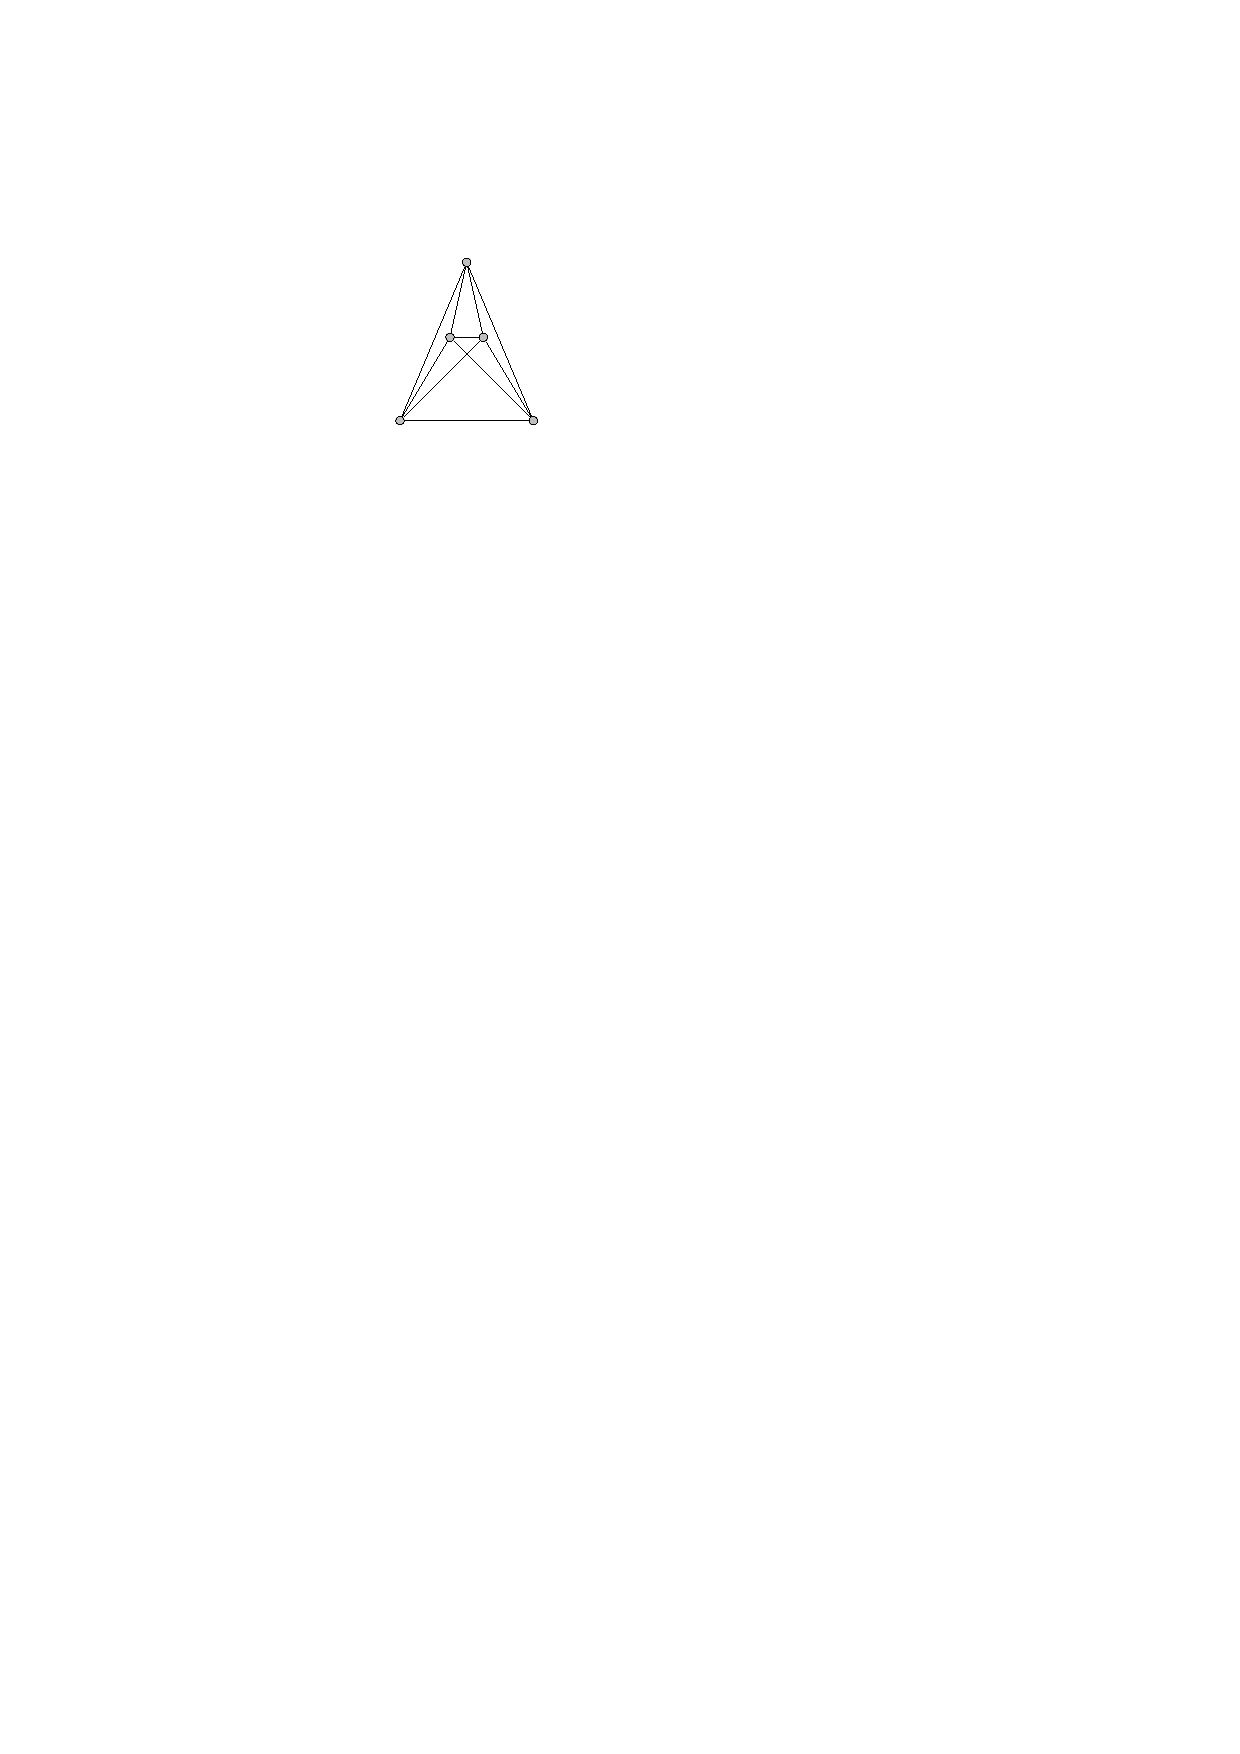
\includegraphics[page=1]{figures/examples}}
	\hfil
	\subfloat[\label{fig:k6} {}]{
	\includegraphics[page=2]{figures/examples}}
	\caption{Illustration of: %
	(a)~a RAC drawing of the complete graph $K_5$, and
	(b)~a drawing of the complete graph $K_6$, whose crossing resolution is arbitrarily close to $90^\circ$.}
	\label{fig:examples}
\end{figure}

The latter result is an indication that the problem of finding drawings with high crossing resolution might also be difficult, even though, formally, its complexity has not been settled yet for values of the crossing resolution smaller than $90^\circ$. It is also worth noting that the literature is significantly more limited, when restricting the crossing resolution to be smaller than $90^\circ$, as also evidenced by Section~\ref{sec:relatedwork}.

From a practical point of view, we are only aware of two methods that aim at drawings with high crossing resolution; both of them are adjustments of force-directed algorithms~\cite{DBLP:journals/congnum/Eades84}. The first one is due to Argyriou et al.~\cite{DBLP:journals/cj/ArgyriouBS13}, while the~second one is due to Huang et al.~\cite{DBLP:journals/vlc/HuangEHL13}. Common in both algorithms is that they apply appropriate forces on the endvertices of every pair of crossing edges. Each of them uses a different way to compute (the direction and the magnitude of) the forces, but the underlying idea of both is the same: the smaller the crossing angles are, the larger are the magnitudes of the forces applied at their endvertices.

In this work, we approach the crossing resolution maximization problem from a different perspective. We suggest a simple and intuitive randomization method for computing drawings with high crossing resolution, which, in a sense, mimics the way a human would try to increase the crossing resolution of a drawing. How would one increase the crossing resolution of a given drawing? First, she would try to identify the pair of edges that define the crossing resolution of the drawing (we call them \emph{critical} edges); then, she would try to move an endvertex of this pair (which we choose at random), hoping that by this move the crossing resolution will increase. Of course, we cannot consider all possible positions for the vertex to be moved. Instead, we consider a small set of randomly generated ones. If there exists a position among them, that does not lead to a reduction of the crossing resolution, we move the vertex to this position.

Note that, in general, randomization is a technique that has not been deeply examined in Graph Drawing, as it seems difficult to even speculate about the expected quality of the produced drawings; a notable exception is the randomized approach by Goldschmidt and Takvorian~\cite{DBLP:journals/networks/GoldschmidtT94} for computing large planar subgraphs of general graphs. Since we also could not provide any theoretical guarantee on the expected quality of the produced drawings (mainly due to the nature of the problem itself), we followed a more practical approach. We implemented our algorithm and the force-directed ones by Argyriou et al.~\cite{DBLP:journals/cj/ArgyriouBS13} and by Huang et al.~\cite{DBLP:journals/vlc/HuangEHL13}, and we experimentally compared them on standard benchmark graphs that are widely used in Graph Drawing for comparing different drawing algorithms. Our evaluation indicates that our method significantly outperforms the aforementioned force-directed algorithms in terms of crossing resolution, but this comes at the cost of slightly worse running time, especially for large and dense graphs. Analogous results are obtained, when our algorithm and the ones by Argyriou et al.~\cite{DBLP:journals/cj/ArgyriouBS13} and by Huang et al.~\cite{DBLP:journals/vlc/HuangEHL13} are adjusted to maximize the \emph{angular resolution} (that is, the minimum value of the angle between any two adjacent edges~\cite{DBLP:journals/siamcomp/FormannHHKLSWW93}) or the \emph{total resolution} (that is, the minimum of the angular and the crossing resolution~\cite{DBLP:journals/cj/ArgyriouBS13}).

\paragraph{Preliminaries:}
Unless otherwise specified, in this paper we consider simple undirected graphs. Let $G=(V,E)$ be such a graph. The degree of vertex $u\in V$ of $G$ is denoted by $d(u)$. The degree $d(G)$ of  graph $G$ is defined as the maximum degree of its vertices, i.e., $d(G)=\max_{u\in V}d(u)$. Given a drawing $\Gamma(G)$ of $G$, we denote by $p(u)=(x_u,y_u)$ the position of vertex $u \in V$ of $G$ in $\Gamma(G)$. 

\paragraph{Structure of the paper:}
The remainder of this paper is structured as follows. Section~\ref{sec:relatedwork} overviews related works. Our algorithm is presented in detail in Section~\ref{sec:algorithm} and is experimentally evaluated against the ones by Argyriou et al.~\cite{DBLP:journals/cj/ArgyriouBS13} and by Huang et al.~\cite{DBLP:journals/vlc/HuangEHL13} in Section~\ref{sec:experiments}, where we also discuss our insights from this project. We conclude in Section~\ref{sec:conclusions} with a discussion of useful observations and insights that we obtained while working on this project.

% ==================================================================
\section{Related Work}
\label{sec:relatedwork}
% ==================================================================

As already mentioned, the study of the crossing resolution maximization problem has mainly focused on (properties of) RAC graphs, that is, on the optimal case of the crossing resolution maximization problem. Their study was initiated by Didimo et al.~\cite{DBLP:journals/tcs/DidimoEL11}, who showed that an $n$-vertex RAC graph has at most $4n-10$ edges~\cite{DBLP:journals/tcs/DidimoEL11}, while deciding whether a graph is RAC is NP-hard~\cite{DBLP:journals/jgaa/ArgyriouBS12}. The maximally-dense RAC graphs are 1-planar~\cite{DBLP:journals/dam/EadesL13}, i.e., they can be drawn with at most one crossing per edge. Actually, several relationships between the class of RAC graphs and subclasses of 1-planar graphs are known~\cite{DBLP:journals/dam/BachmaierBHNR17,DBLP:journals/tcs/BrandenburgDEKL16}. Deciding, however, whether a $1$-planar graph is RAC is NP-hard~\cite{DBLP:journals/tcs/BekosDLMM17}. Note that the problem of finding RAC drawings has also been studied in the presence of bends~\cite{DBLP:journals/jgaa/AngeliniCDFBKS11,DBLP:journals/comgeo/ArikushiFKMT12,DBLP:journals/tcs/DidimoEL11,DBLP:journals/mst/GiacomoDLM11} and by imposing restrictions on the degree~\cite{DBLP:conf/s-egc/AngeliniBDFHKLL11}, the structure~\cite{DBLP:journals/ipl/DidimoEL10} and the drawing~\cite{DBLP:journals/algorithmica/GiacomoDEL14,DBLP:conf/wg/HongN15} of the graph. 

The results are fewer, when the right-angle constraint is relaxed. To the best of our knowledge, there is only one work, by Dujmovic et al.~\cite{DBLP:journals/cjtcs/DujmovicGMW11}, which studies the crossing resolution maximization problem by relaxing the right-angle constraint on the crossing angles of the computed drawings. More precisely, in their work, Dujmovic et al.~\cite{DBLP:journals/cjtcs/DujmovicGMW11} proved that an $n$-vertex graph, whose crossing resolution is at least $\alpha$ (in radians) has at most $(3n-6)\pi/\alpha$ edges. Corresponding density results for the case, in which few bends are allowed along each edge, are known by Ackerman et al.~\cite{DBLP:journals/siamdm/AckermanFT12} and Di Giacomo et al.~\cite{DBLP:journals/mst/GiacomoDLM11}.

An immediate observation emerging from the above overview is that the focus has been primarily on theoretical aspects of the problem. Most of the approaches that could be useful in practice are based on adjustments of force-directed techniques~\cite{DBLP:journals/congnum/Eades84}, according to which a graph is modelled as a physical system with forces acting on it, and a (good) drawing is obtained by an equilibrium of the system; for an introduction and a discussion of several variants we point the reader to~\cite{DBLP:books/ph/BattistaETT99}. 

More concretely, from an applicative point of view, Didimo et al.~\cite{DBLP:conf/apvis/DidimoLR10} describe a system, called \emph{COWA},  to support conceptual web site traffic analysis~\cite{DBLP:conf/apvis/DidimoLR10}; its algorithmic core is a force-directed heuristic to compute simultaneous embeddings of two non-planar graphs with high crossing resolution.
%
In a follow up work, Didimo et al.~\cite{DBLP:conf/gd/DidimoLR10} describe heuristics, designed within the topology-driven force-directed framework, to achieve good trade-offs in terms of number of edge crossings, crossing resolution, and geodesic edge tendency.
%
However, the obtained drawings are not straight-line. For straight-line drawings, Nguyen et al.~\cite{DBLP:conf/gd/NguyenEHH10} suggest a quadratic-programming based approach to increase the crossing angles of circular drawings. However, its usefulness is only limited to small graphs and to a specific kind of drawings.

Of more general scope are, of course, the already mentioned works by Argyriou et al.~\cite{DBLP:journals/cj/ArgyriouBS13} and by Huang et al.~\cite{DBLP:journals/vlc/HuangEHL13}, which are also based on the force-directed technique.

% ==================================================================
\section{Description of our Heuristic Approach}
\label{sec:algorithm}
% ==================================================================

In this section, we describe our heuristic for obtaining drawings with high crossing resolution. The input of our heuristic consists of a graph $G$ and an initial drawing $\Gamma_0$ of $G$ with crossing resolution $c(\Gamma_0)$. We assume that no two edges of graph $G$ overlap in drawing $\Gamma_0$, i.e., $c(\Gamma_0)>0$. A circular drawing or a drawing obtained by applying a force-directed algorithm on graph $G$ clearly meets this precondition.

Our algorithm is iterative and at each iteration performs some operations that are mainly based on randomization. At the $i$-th iteration, we assume that we have computed a drawing $\Gamma_{i-1}$ of graph $G$ of crossing resolution $c(\Gamma_{i-1}) \geq c(\Gamma_0)$. In other words, we assume, as an invariant for our algorithm, that the crossing resolution cannot be decreased at some iteration of our algorithm (so, in a sense, our algorithm resembles probabilistic hill climbing approaches). We proceed by choosing a vertex of $\Gamma_{i-1}$ arbitrarily at random based on the content of the so-called \emph{vertex-pool}, which may contain:

\begin{itemize}
\item[--] either a prespecified subset of the vertices of $\Gamma_{i-1}$, called \emph{critical}, or
\item[--] all vertices of $\Gamma_{i-1}$.
\end{itemize}

Intuitively, the critical vertices are the endpoints of the edges that define the crossing resolution of drawing $\Gamma_{i-1}$. To formally define them, we first need to introduce the notion of critical edge-pairs. A pair of edges $e$ and $e'$ is called \emph{critical} in drawing $\Gamma_{i-1}$ if and only if edges $e$ and $e'$ cross in $\Gamma_{i-1}$ and the minimum angle that is formed at their crossing point is equal to the crossing resolution of drawing $\Gamma_{i-1}$ (that is, to $c(\Gamma_{i-1})$). The set of critical vertices of drawing $\Gamma_{i-1}$ is then defined by the four endvertices of each critical edge-pair.

The role of critical vertices is central in our algorithm\footnote{If the focus is not on the critical vertices for a large graph, then our algorithm will need a large number of iterations to converge to a solution with good crossing resolution, because it is simply very unlikely to select to move one of the vertices that define the crossing resolution.}: By appropriately changing the location of a critical vertex or of a vertex that is in the neighbourhood of the critical vertices, we naturally expect to improve the crossing resolution of the current drawing. We turned this observation into an algorithmic implementation through a probabilistic random selection procedure, so that the vertices at graph-distance~$i$ from the ones of the vertex-pool have higher probability for selection than the corresponding ones at graph-distance~$j$  in $G$, when $0 \leq i<j$. In other words, the closer a vertex is to the critical vertices, the more likely it is to be chosen. On the other hand, if the vertex-pool contains all vertices of the graph, then each vertex can be chosen with the same probability.

What we quickly realized from our practical analysis, is that the crossing resolution of the initial drawing improves rapidly during the first iterations of the algorithm. However, by focusing only at the critical vertices, it is highly possible that the algorithm will get trapped to some local maxima after a number of iterations. Therefore, special care is needed to avoid these bottlenecks, especially when the input graph is large. We will discuss ways to avoid local maxima later in this section (refer to subsection~\ref{ssec:bottlenecks}).

So far, we have described the main idea of our algorithm, which at each iteration chooses uniformly at random a vertex of the current drawing to move (based on the content of the vertex-pool), so to improve the crossing resolution. Next, we describe how to compute the new position of the chosen vertex in the next drawing $\Gamma_i$. Recall that the crossing resolution $c(\Gamma_{i})$ of drawing $\Gamma_{i}$ that is obtained after the $i$-th iteration of the algorithm must be at least as large as the crossing resolution $c(\Gamma_{i-1})$ of drawing $\Gamma_{i-1}$ (by the invariant of our algorithm), that is, $c(\Gamma_i) \ge c(\Gamma_{i-1})$. 

Let $v_i$ be the vertex of drawing $\Gamma_{i-1}$ that has been chosen to be moved at the $i$-th iteration. To compute the position of vertex $v_i$ in the next drawing $\Gamma_i$, we consider a set of $\rho$ rays $r_0,r_1,\ldots,r_{\rho-1}$ that all emanate from $p(v_i)$ in $\Gamma_{i-1}$, such that the angle formed by ray $r_j$, with $j=0,1,\ldots,\rho-1$, and the horizontal axis equals to $2j\pi/\rho$, where $\rho>0$ is an integer parameter of the algorithm. These rays are then rotated by an angle that is chosen uniformly at random in the interval $[0,2\pi]$; see Fig.~\ref{fig:algo} for an illustration. The position of vertex $v_i$ in $\Gamma_i$ will eventually be along one of the rays $r_0,r_1,\ldots,r_{\rho-1}$. More precisely, for each ray $r_i$ we choose a distance value $\delta_i$ uniformly at random from the interval $[\delta_{min},\delta_{max}]$, where $\delta_{min}$ and $\delta_{max}$ are two positive parameters of the algorithm. For each $j=0,1,\ldots,\rho-1$, a new point $\pi_j$ is obtained by translating $p(u)$ along $r_j$ by a distance $\delta_j$; we call point $\pi_j$ \emph{feasible} if and only if there is no vertex of drawing $\Gamma_{i-1}$ at point $\pi_j$ and the crossing resolution of the drawing obtained by placing vertex $v_i$ at point $\pi_j$ and by keeping all other vertices of the graph in their positions in $\Gamma_{i-1}$ is at least as large as the crossing resolution of $\Gamma_{i-1}$.

\begin{figure}[t!]
	\centering
	\subfloat[\label{fig:algo-rays} {}]{
	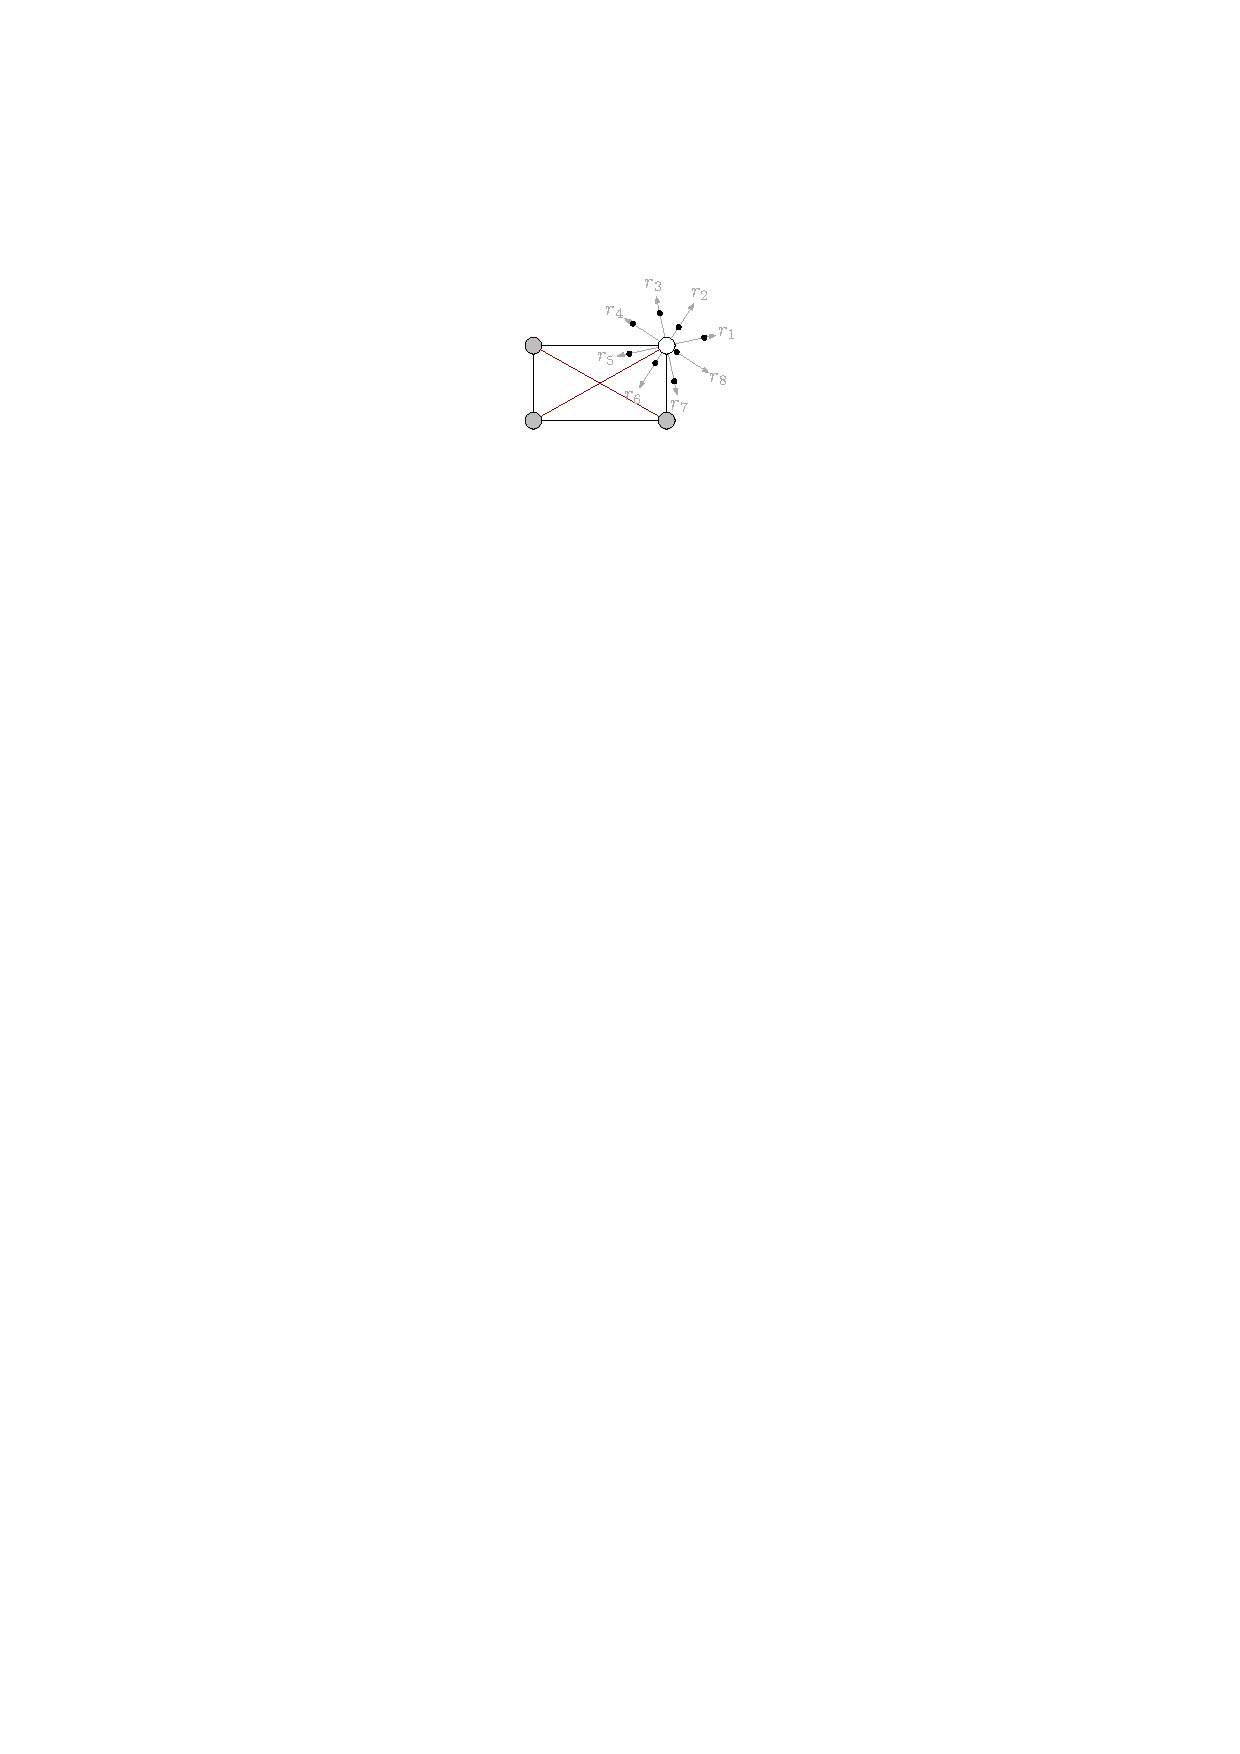
\includegraphics[page=1]{figures/algorithm}}
	\hfil
	\subfloat[\label{fig:algo-move} {}]{
	\includegraphics[page=2]{figures/algorithm}}
	\caption{%
	Illustration of an iteration step of our algorithm:
	(a)~the chosen vertex is the white one;
	the computed rays $r_0,\ldots,r_7$ have been rotated by $8^\circ$;
	the black-colored points along these rays are points $\pi_0,\ldots,\pi_7$;
	among them, $\pi_4$ yields the best solution, and
	(b)~the resulting drawing after moving the vertex at position $\pi_2$.}
	\label{fig:algo}
\end{figure}

If none of the points $\pi_j$, with $j=0,1,\ldots,\rho-1$ is feasible, then the position of $v_i$ in $\Gamma_i$ is $p(v_i)$, i.e., the same as in $\Gamma_{i-1}$, since $c(\Gamma_i) \geq c(\Gamma_{i-1})$ must hold. If there is one or more feasible points, then one may consider two different approaches to determine the position of vertex $v_i$ in $\Gamma_i$. The most natural is to choose the feasible point that maximizes the crossing resolution of the obtained drawing. As an alternative, one may rely again on randomization and chose uniformly at random one of the feasible points as the position of vertex $v_i$ in $\Gamma_i$. We note that we did not observe any significant difference between these two approaches (in terms of the crossing resolution of the obtained drawings), so we simply adopted the first one. The termination condition of our algorithm is simple and depends on an input parameter $\tau$. More specifically, if the crossing resolution has not improved during the last $\tau$ iterations, we assume that the algorithm has converged and we stop.

% ==================================================================
\subsection{Avoiding local maxima}
\label{ssec:bottlenecks}
% ==================================================================
%
To avoid getting trapped to locally optimal solutions, we mainly investigated two approaches, which are both  parametrizable by two input parameters $\zeta$ and $\zeta'$. The first mimics the human behavior. What would one do to escape from a locally optimal solution? She would stop trying to move the endvertices of the edges defining the crossing resolution; she would rather start moving ``irrelevant'' vertices hoping that by doing so a better solution will be easier to be computed afterwards. Our algorithm is mimicking this idea as follows:
%
\begin{itemize}
\item[--] if during the last $\zeta$ iterations the crossing resolution has not been~improved, then the vertex-pool becomes \emph{wider} by including all the vertices, and the algorithm is executed with this vertex-pool for $\zeta'$ iterations;
\item[--] afterwards, the vertex-pool switches back to the critical vertices.
\end{itemize}

From our extensive practical analysis, we quickly realized that, while this approach turned out to be effective for smaller graphs, for graphs with more than 100 vertices, it was not so efficient; in most iterations with the wider vertex-pool, the embedding could not change in a beneficial way for the algorithm to proceed.

Our second approach is based on parameters $\rho$, $\delta_{min}$ and $\delta_{max}$ of the algorithm. Our idea was that if the algorithm gets trapped to a locally optimal solution, then a ``drastic'' or ``sharp'' move may help to escape. We turned this idea into an algorithmic implementation as follows:
%
\begin{itemize}
\item[--] if during the last $\zeta$ iterations the crossing resolution has not been improved, we double the values of $\rho$, $\delta_{min}$ and $\delta_{max}$, and the algorithm is executed with these values for $\zeta'$ iterations;
\item[--] afterwards, $\rho$, $\delta_{min}$ and $\delta_{max}$ switch back to this initial value.
\end{itemize}

Note, however, that this approach may lead to drawings with larger area, but this is ``expected'', as it turns out that drawings with high crossing resolution may require large area~\cite{DBLP:journals/jgaa/AngeliniCDFBKS11,DBLP:journals/tcs/BrandenburgDEKL16}.

% ==================================================================
\subsection{Complexity issues}
\label{ssec:complexity}
% ==================================================================

A factor that highly affects the efficiency of our algorithm is the computation of the crossing points of the edges and the corresponding angles at these points. Given  a drawing, a na\"ive approach to compute its crossings requires $O(m^2)$ time, which can be improved by a plane-sweep technique to $O(m \log m + c)$ time, where $m$ and $c$ denote the number of edges and crossings; see, e.g.,~\cite{DBLP:books/lib/BergCKO08}.

Instead of computing all crossing points and the corresponding angles for each candidate position of each iteration, we adopted a different approach for determining the set of feasible candidate positions, which turned out to be quite efficient in practice. Recall that we denoted by $v_i$ the vertex chosen at the $i$-th iteration step, and by $\pi_0,\ldots,\pi_{\rho-1}$ the candidate positions to move $v_i$. Let $e_0,\ldots,e_{d_i-1}$ be the edges incident to $v_i$, where $d_i$ denotes the degree of vertex $v_i$. Next, for each edge $e_k$ with $k=0,\ldots,d_i-1$ we compute the crossings and the corresponding crossing angles of edge $e_k$ with all other edges in $\Gamma_{i-1}$. Let $\phi_i$ be the minimum crossing angle computed; this is our reference angle. Also, for each candidate position $\pi_j$ with $j=0,\ldots,\rho-1$, and for each edge $e_k$ with $k=0,\ldots,d_i-1$, we compute the crossings and the corresponding crossing angles of $e_k$ with all other edges of the drawing, assuming that vertex $v_i$ is at position $\pi_j$. Let $\chi_j$ be the minimum crossing angle computed with this approach, when vertex $v_i$ is at position $\pi_j$. Clearly, $\pi_j$ is feasible, only if $\chi_j \geq \phi_i$. Note that the complexity of this approach is $O(\deg(v_i)m) = O(nm)$.

% ==================================================================
\subsection{Some Interesting Variants}
\label{ssec:variants}
% ==================================================================

In general, aesthetically pleasant drawings of graphs are usually the result of compromising between different aesthetic criteria. Towards this direction, we discuss in this section interesting variants of our algorithm, which are motivated by the following observation that we made while working on this project (see Section~\ref{sec:conclusions}): Drawings that are optimised only in terms of the crossing resolution tend to have bad aspect ratio (that is, the ratio of the longest to the shortest edge is large) and poor angular resolution (that is, the angles formed by adjacent edges are small). The former seems to be a consequence of the fact that drawings with good crossing resolution tend to be quite demanding in area. For the latter, observe that if in a drawing all edges are either almost horizontally or almost vertically drawn, such that only ``horizontal'' and ``vertical'' edges cross, then the crossing resolution of this drawing is arbitrarily close to $90^\circ$, while its angular resolution is arbitrarily close to~$0^\circ$.

% ==================================================================
\myparagraph{Aspect ratio}
% ==================================================================
%
Formally, the aspect ratio of a drawing is the ratio of the length of its longest edge to the length of its shortest edge. Sometimes it is also used as a measure of the area of non-grid drawings. It was easy to instruct our algorithm to prevent producing drawings with aspect ratio either higher than the one of the starting layout or higher than a given input value. What we simply had to do was to reject candidate positions, which violate this precondition.

% ==================================================================
\myparagraph{Total resolution}
% ==================================================================
%
The notion of the total resolution of a drawing was introduced relatively recently with aim of ``balancing'' the measures of the crossing and of the angular resolution of a drawing~\cite{DBLP:journals/cj/ArgyriouBS13}. Formally, it is defined as the minimum of these two measures. It was not difficult to adjust our algorithm to yield drawings with high total resolution by simply taking into account also the angular resolution of the drawing. In particular, if the total resolution of the drawing is defined by its angular resolution, then the way we compute the critical vertices of this drawing has to change; the critical vertices must be the endvertices of the pairs of edges that define the angular resolution. Also, at each iteration of our algorithm we have to ensure that the total resolution does not decrease. We do so by rejecting candidate positions which yield a reduced total~resolution.

% ==================================================================
\myparagraph{Angular resolution}
% ==================================================================
%
As it is the case with the force-directed algorithms by Argyriou et al.~\cite{DBLP:journals/cj/ArgyriouBS13} and by Huang et al.~\cite{DBLP:journals/vlc/HuangEHL13}, our algorithm can also be restricted to maximize only the angular resolution (by neglecting its crossing resolution). We already described in the previous paragraph the necessary changes in the definition of the critical vertices and the rule according to which a candidate position is rejected (i.e., when it yields a drawing with a reduced angular resolution).

% ==================================================================
\myparagraph{Grid drawings}
% ==================================================================
%
Our algorithm, as it has been described so far, does not necessarily produce grid drawings, i.e., drawings in which the vertices are at integer coordinates. However, it can be easily adjusted to produce such drawings. More precisely, if we round the candidate positions computed at each iteration of our algorithm to their closest grid points and use these grid points as candidates for the next position of the vertex to be moved, then the obtained drawing will be grid (assuming, of course, that the starting drawing is grid). One can even bound the size of the grid, by rejecting candidate grid positions that lie outside the permitted bounds. 

Note that an alternative approach is to let our algorithm compute a (non-grid) drawing and then apply some technique to convert it to grid. However, critical in this step is not to affect the crossing resolution of the computed drawing too much during its conversion to grid. It is worth noting that we tried to apply such a technique (using again randomization). Our idea was to choose uniformly at random, for each vertex of the non-grid starting drawing, one of the grid points from its \emph{neighbourhood}, and move it to this point (assuming of course that there is no other vertex at this point), where the neighbourhood of the vertex was initially set to its four closest grid points. If after a number of iterations a grid drawing without vertex-vertex overlaps and of similar crossing resolution as the one of the starting drawing could not be reported, then we had to augment the neighbourhood of each vertex so to contain more grid points (hoping that by this augmentation the computation of an acceptable grid drawing will be become feasible). 

However, we faced two main difficulties when adopting this alternative approach. First, we could not always guarantee that the crossing resolution of the final grid drawing will be similar to the one of the starting drawing without increasing the drawing area too much. The second one is that the conversion itself is an extra step in the algorithm, which some times was more demanding than the main step of the algorithm, which was the actual computation of the drawing with high crossing resolution. So, we decided not to adopt this alternative approach.

% ==================================================================
\section{Experimental Evaluation}
\label{sec:experiments}
% ==================================================================

In this section, we present the results of our experimental evaluation. For comparison purposes, apart from our algorithm, we also implemented the force-directed algorithms by Argyriou et al.~\cite{DBLP:journals/cj/ArgyriouBS13} and by Huang et al.~\cite{DBLP:journals/vlc/HuangEHL13}. The implementations\footnote{All implementations are available on request by the authors.} were in Java using the yFiles graph drawing library~\cite{DBLP:books/sp/04/WieseE004}. 

% ==================================================================
\subsection{Experiment's Setup}
\label{ssec:setup}
% ==================================================================

As test sets for our experiment, we used the non-planar Rome graphs~\cite{DBLP:reference/crc/BattistaD13} and the non-planar AT\&T graphs (also known as Graph Catalog or North graphs; available at \texttt{http://graphdrawing.org/data}), which are two collections of around 8.100 and 424 benchmark graphs, respectively, that are widely used in Graph Drawing for the evaluation of different drawing algorithms. 

The experiment was performed on a Linux laptop with four cores at 2.4 GHz and 8 GB RAM. The experiment was performed as follows. Initially, each graph of our expertiment was laid out using the SmartOrganic layouter of yFiles~\cite{DBLP:books/sp/04/WieseE004}. Starting from this layout, every graph was drawn with:
%
\begin{itemize}
\item[--] our algorithm with $\delta_{max}=\frac{1}{2}\max\{w,h\}$, where $w$ and $h$ are the width and the height of the initial drawing, respectively, $\delta_{min}=\frac{1}{100}\delta_{max}$ and $\rho=10$,
\item[--] our algorithm restricted not to violate the aspect ratio of the initial layout, 
\item[--] the force-directed algorithm by Argyriou et al., and
\item[--] the force-directed algorithm by Huang et al.
\end{itemize}

Since all algorithms of the experiment can easily be adjusted to maximize~only the crossing resolution, or only the angular resolution or both (by maximizing~the total resolution), we adjusted each of them to maximize exclusively the corresponding measures. In our algorithm, this can be achieved by modifying appropriately the content of the vertex-pool (as we discussed in Section~\ref{ssec:variants}), while in the algorithms of Argyriou et al.\ and of Huang et al.\ by switching on only the forces that maximize the corresponding properties under measure (note that, each of these two algorithms has a different set of forces to maximize the crossing and the angular resolution, such that together they maximize the total resolution). The reported results, illustrated in Figures~\ref{fig:cr-res}--\ref{fig:northAngular}, are on average across different drawings with same number of vertices.

% ==================================================================
\subsection{The Rome Graph Test Set}
\label{ssec:rome}
% ==================================================================

In this subsection, we report the results of our expertimental evaluation for the non-planar Rome graphs. Note that we did not impose any grid constraint on our algorithms. Our results are summarized in Figures~\ref{fig:cr-res}, \ref{fig:an-res} and~\ref{fig:to-res}.

\myparagraph{Crossing resolution} Our results for the crossing resolution are summarized in Fig.~\ref{fig:cr-res}. Here, each algorithm was adjusted to maximize exclusively the crossing resolution (i.e., by ignoring the drawing's angular resolution). It is immediate to see that our algorithm outperforms all other ones in terms of the crossing resolution of the produced drawings, when we do not impose any restriction on the aspect ratio of the computed drawings; refer to the solid-black curve, denoted as \emph{Unrestricted}, in Fig.~\ref{fig:cr-res-1}. The variant of our algorithm, which does not violate the aspect ratio of the initial layout, leads to drawings with slightly smaller crossing resolution; refer to the solid-gray curve, denoted as \emph{AR-restricted}, in Fig.~\ref{fig:cr-res-1}. Finally, the two force-directed algorithms seem to produce drawings with worse crossing resolution; refer to the dotted-gray and dotted-black curves of Fig.~\ref{fig:cr-res-1} (by Argyriou et al.\ and by Huang et al., respectively).

% ==================================================================
%\begin{figure*}[t]
\centering
\subfloat[\label{fig:cr-res-1}{Crossing resolution vs no.~of vertices}]{
\centering
%======================
% Crossing Resolution
%======================
\begin{tikzpicture}
\begin{axis}[axis x line*=bottom,xlabel style={yshift=0.2cm},axis y line*=left,ylabel style={yshift=-0.2cm}, legend style={at={(0.425,1.35)},anchor=north,legend columns=2,draw=none}, width=0.475\textwidth, cycle list name=mylist,
mark repeat={5}, xtick={10,20,30,40,50,60,70,80,90,100}, ytick={0,10,20,30,40,50,60,70,80,90}, ylabel={Crossing Resolution}, xlabel={Number of Vertices}, xmin=10, xmax=100, tick pos=left,ymajorgrids]
\addplot table [x=n, y=crossing resolution rm, col sep=semicolon]{crossingResolution.csv};
\addplot table [x=n, y=crossing resolution rm-1, col sep=semicolon] {crossingResolution.csv};
\addplot table [x=n, y=crossing resolution fa, col sep=semicolon]{crossingResolution.csv};
\addplot table [x=Nodes, y=Crossing Only, col sep=semicolon]{abs-crossingResolution.csv};
\legend{{Unrestricted},{AR-restricted~~},{Huang et al.},{Argyriou et al.}}
\end{axis}
\end{tikzpicture}}
\subfloat[\label{fig:cr-res-2}{Aspect ratio vs no.~of vertices}]{
\centering
%===================================
% Crossing Resolution Aspect Ratio
%===================================
\begin{tikzpicture}
\begin{axis}[axis x line*=bottom,xlabel style={yshift=0.2cm},axis y line*=left,ylabel style={yshift=-0.2cm},legend style={at={(0.425,1.35)}, anchor=north,legend columns=2,draw=none}, width=0.475\textwidth,cycle list name=mylist, mark repeat={5},xtick={10,20,30,40,50,60,70,80,90,100},ylabel={Aspect Ratio}, xlabel={Number of Vertices}, ytick={1,2.5,10,25,100,250,1000,2500,10000}, xmin=10, xmax=100,ymode=log, log ticks with fixed point,tick pos=left, ymajorgrids,]
\addplot table [x=n, y=Aspect ratio rm, col sep=semicolon]{crossingResolution.csv};
\addplot table [x=n, y=Aspect ratio rm-1, col sep=semicolon] {crossingResolution.csv};
\addplot table [x=n, y=Aspect ratio fa, col sep=semicolon]{crossingResolution.csv};
\addplot table [x=Nodes, y=Crossing Only, col sep=semicolon]{abs-aspectRatio.csv};
\legend{{Unrestricted},{AR-restricted~~},{Huang et al.},{Argyriou et al.}}
\end{axis}
\end{tikzpicture}}

\subfloat[\label{fig:cr-res-3}{No.~of crossings vs no.~of vertices}]{
\centering
%======================================
% Crossing Resolution Crossing Number
%======================================
\begin{tikzpicture}
\begin{axis}[axis x line*=bottom,xlabel style={yshift=0.2cm},axis y line*=left,ylabel style={yshift=-0.2cm},legend style={at={(0.425,1.35)}, anchor=north,legend columns=2,draw=none}, width=0.475\textwidth,cycle list name=mylist,  mark repeat={5},xtick={10,20,30,40,50,60,70,80,90,100}, xmin=10, xmax=100, ytick={0,25,50,75,100,125,150,175,200},ylabel={Number of Crossings}, xlabel={Number of Vertices},tick pos=left, ymajorgrids]
\addplot table [x=n, y=Crossing number rm, col sep=semicolon]{crossingResolution.csv};
\addplot table [x=n, y=Crossing number rm-1, col sep=semicolon] {crossingResolution.csv};
\addplot table [x=n, y=Crossing number fa, col sep=semicolon]{crossingResolution.csv};
\addplot table [x=Nodes, y=Crossing Only, col sep=semicolon]{abs-crossings.csv};
\legend{{Unrestricted},{AR-restricted~~},{Huang et al.},{Argyriou et al.}}
\end{axis}
\end{tikzpicture}}
\subfloat[\label{fig:cr-res-4}{No.~of iterations vs no.~of vertices}]{
\centering
%==================================
% Crossing Resolution Iterations
%==================================
\begin{tikzpicture}
\begin{axis}[axis x line*=bottom,xlabel style={yshift=0.2cm},axis y line*=left,ylabel style={yshift=-0.2cm},legend style={at={(0.425,1.35)}, anchor=north,legend columns=2,draw=none}, width=0.475\textwidth,cycle list name=mylist,  ylabel={Iterations}, xlabel={Number of Vertices}, mark repeat={5},xtick={10,20,30,40,50,60,70,80,90,100}, xmin=10,
xmax=100, ytick={0,500,1000,1500,2000,2500,3000,3500,4000,4500,5000},tick pos=left, ymajorgrids]
\addplot table [x=n, y=Iterations rm, col sep=semicolon]{crossingResolution.csv};
\addplot table [x=n, y=Iterations rm-1, col sep=semicolon] {crossingResolution.csv};
\addplot table [x=n, y=Iterations fa, col sep=semicolon]{crossingResolution.csv};
\addplot table [x=Nodes, y=Crossing Only, col sep=semicolon]{abs-iterations.csv};
\legend{{Unrestricted},{AR-restricted~~},{Huang et al.},{Argyriou et al.}}
\end{axis}
\end{tikzpicture}}
\caption{Experimental results on the crossing resolution for the Rome graphs.}
\label{fig:cr-res}
\end{figure*}
% ==================================================================
\begin{figure*}[t]
	\centering
	\subfloat[\label{fig:cr-res-1}{Crossing resolution vs no.~of vertices}]{
	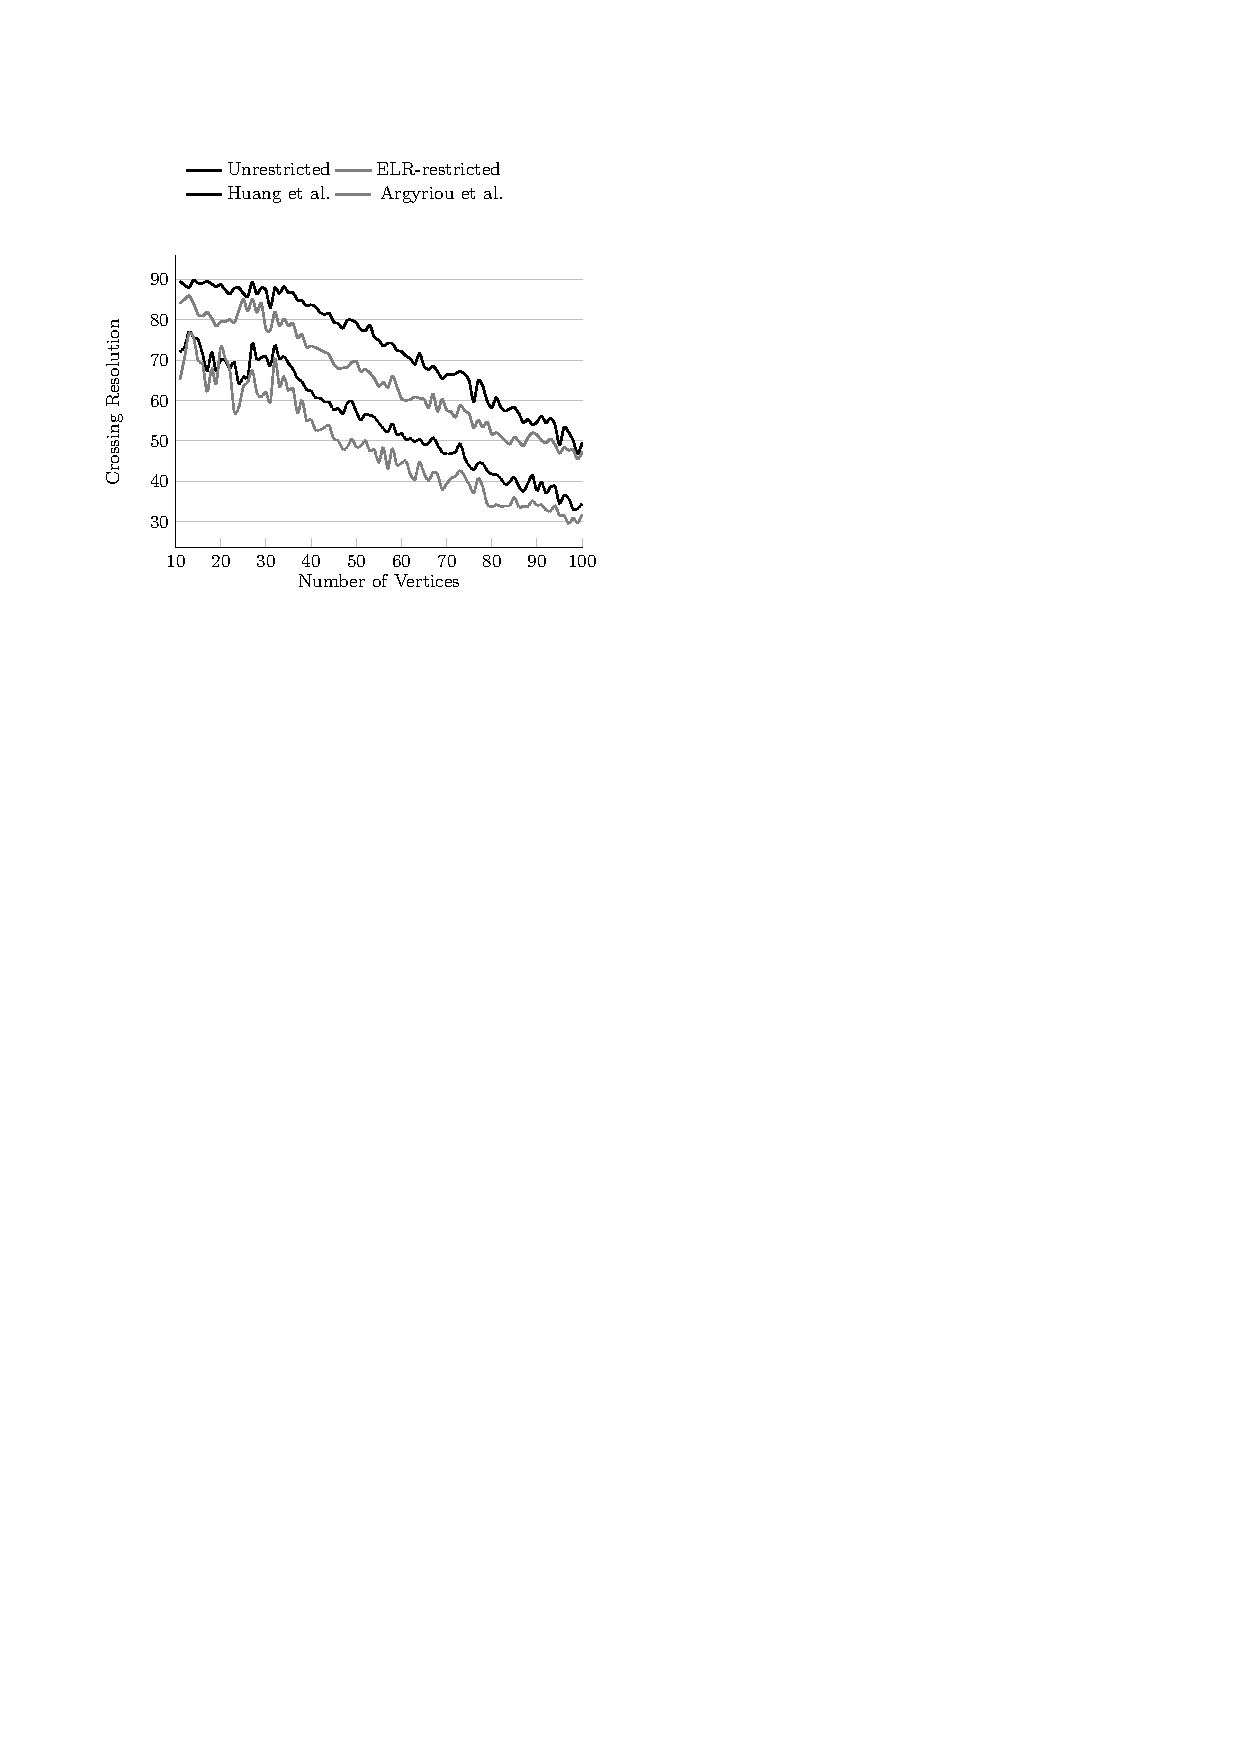
\includegraphics[scale=0.99,page=1]{figures/rome}}
	\hfil
	\subfloat[\label{fig:cr-res-2}{Aspect ratio vs no.~of vertices}]{
	\includegraphics[scale=0.99,page=2]{figures/rome}}
	
	\subfloat[\label{fig:cr-res-3}{No.~of crossings vs no.~of vertices}]{
	\includegraphics[scale=0.99,page=3]{figures/rome}}
	\hfil
	\subfloat[\label{fig:cr-res-4}{No.~of iterations vs no.~of vertices}]{
	\includegraphics[scale=0.99,page=4]{figures/rome}}
	\caption{Experimental results on the crossing resolution for the Rome graphs.}
	\label{fig:cr-res}
\end{figure*}

% ==================================================================
%\begin{figure*}[t]
\centering
\subfloat[\label{fig:to-res-1}{Total resolution vs no.~of vertices}]{
\centering
%======================
% Total Resolution
%======================
\begin{tikzpicture}
\begin{axis}[axis x line*=bottom,xlabel style={yshift=0.2cm},axis y line*=left,ylabel style={yshift=-0.2cm}, legend style={at={(0.425,1.35)},anchor=north,legend columns=2,draw=none}, width=0.475\textwidth, cycle list name=mylist,
mark repeat={5}, xtick={10,20,30,40,50,60,70,80,90,100}, ytick={0,10,20,30,40,50,60,70,80,90}, ylabel={Total Resolution}, xlabel={Number of Vertices}, xmin=10, xmax=100, tick pos=left,ymajorgrids]
\addplot table [x=n, y=Total Resolution rm, col sep=semicolon]{totalResolution.csv};
\addplot table [x=n, y=Total Resolution rm-1, col sep=semicolon] {totalResolution.csv};
\addplot table [x=n, y=Total Resolution fa, col sep=semicolon]{totalResolution.csv};
\addplot table [x=Nodes, y=Mixed, col sep=semicolon]{abs-totalResolution.csv};
\legend{{Unrestricted},{AR-restricted~~},{Huang et al.},{Argyriou et al.}}
\end{axis}
\end{tikzpicture}}
\subfloat[\label{fig:to-res-2}{Aspect ratio vs no.~of vertices}]{
\centering
%===================================
% Total Resolution Aspect Ratio
%===================================
\begin{tikzpicture}
\begin{axis}[axis x line*=bottom,xlabel style={yshift=0.2cm},axis y line*=left,ylabel style={yshift=-0.2cm},legend style={at={(0.425,1.35)}, anchor=north,legend columns=2,draw=none}, width=0.475\textwidth,cycle list name=mylist, mark repeat={5},xtick={10,20,30,40,50,60,70,80,90,100},ylabel={Aspect Ratio}, xlabel={Number of Vertices}, ytick={1,2.5,10,25,100,250,1000,2500,10000}, xmin=10, xmax=100,ymode=log, log ticks with fixed point,tick pos=left, ymajorgrids,]
\addplot table [x=n, y=Aspect ratio rm, col sep=semicolon]{totalResolution.csv};
\addplot table [x=n, y=Aspect ratio rm-1, col sep=semicolon] {totalResolution.csv};
\addplot table [x=n, y=Aspect ratio fa, col sep=semicolon]{totalResolution.csv};
\addplot table [x=Nodes, y=Mixed, col sep=semicolon]{abs-aspectRatio.csv};
\legend{{Unrestricted},{AR-restricted~~},{Huang et al.},{Argyriou et al.}}
\end{axis}
\end{tikzpicture}}

\subfloat[\label{fig:to-res-3}{No.~of crossings vs no.~of vertices}]{
\centering
%======================================
% Total Resolution Crossing Number
%======================================
\begin{tikzpicture}
\begin{axis}[axis x line*=bottom,xlabel style={yshift=0.2cm},axis y line*=left,ylabel style={yshift=-0.2cm},legend style={at={(0.425,1.35)}, anchor=north,legend columns=2,draw=none}, width=0.475\textwidth,cycle list name=mylist,  mark repeat={5},xtick={10,20,30,40,50,60,70,80,90,100}, xmin=10, xmax=100, ytick={0,25,50,75,100,125,150,175,200},ylabel={Number of Crossings}, xlabel={Number of Vertices},tick pos=left, ymajorgrids]
\addplot table [x=n, y=Crossing number rm, col sep=semicolon]{totalResolution.csv};
\addplot table [x=n, y=Crossing number rm-1, col sep=semicolon] {totalResolution.csv};
\addplot table [x=n, y=Crossing number fa, col sep=semicolon]{totalResolution.csv};
\addplot table [x=Nodes, y=Mixed, col sep=semicolon]{abs-crossings.csv};
\legend{{Unrestricted},{AR-restricted~~},{Huang et al.},{Argyriou et al.}}
\end{axis}
\end{tikzpicture}}
\subfloat[\label{fig:to-res-4}{No.~of iterations vs no.~of vertices}]{
\centering
%==================================
% Total Resolution Iterations
%==================================
\begin{tikzpicture}
\begin{axis}[axis x line*=bottom,xlabel style={yshift=0.2cm},axis y line*=left,ylabel style={yshift=-0.2cm},legend style={at={(0.425,1.35)}, anchor=north,legend columns=2,draw=none}, width=0.475\textwidth,cycle list name=mylist,  ylabel={Iterations}, xlabel={Number of Vertices}, mark repeat={5},xtick={10,20,30,40,50,60,70,80,90,100}, xmin=10,
xmax=100, ytick={0,500,1000,1500,2000,2500,3000,3500,4000,4500,5000},tick pos=left, ymajorgrids]
\addplot table [x=n, y=Iterations rm, col sep=semicolon]{totalResolution.csv};
\addplot table [x=n, y=Iterations rm-1, col sep=semicolon] {totalResolution.csv};
\addplot table [x=n, y=Iterations fa, col sep=semicolon]{totalResolution.csv};
\addplot table [x=Nodes, y=Mixed, col sep=semicolon]{abs-iterations.csv};
\legend{{Unrestricted},{AR-restricted~~},{Huang et al.},{Argyriou et al.}}
\end{axis}
\end{tikzpicture}}
\caption{Experimental results on the total resolution for the Rome graphs.}
\label{fig:to-res}
\end{figure*}
% ==================================================================
\begin{figure*}[t]
	\centering
	\subfloat[\label{fig:to-res-1}{Crossing resolution vs no.~of vertices}]{
	\includegraphics[scale=0.99,page=5]{figures/rome}}
	\hfil
	\subfloat[\label{fig:to-res-2}{Aspect ratio vs no.~of vertices}]{
	\includegraphics[scale=0.99,page=6]{figures/rome}}
	
	\subfloat[\label{fig:to-res-3}{No.~of crossings vs no.~of vertices}]{
	\includegraphics[scale=0.99,page=7]{figures/rome}}
	\hfil
	\subfloat[\label{fig:to-res-4}{No.~of iterations vs no.~of vertices}]{
	\includegraphics[scale=0.99,page=8]{figures/rome}}
	\caption{Experimental results on the total resolution for the Rome graphs.}
	\label{fig:to-res}
\end{figure*}

% ==================================================================
%\begin{figure*}[t]
\centering
\subfloat[\label{fig:an-res-1}{Angular resolution vs no.~of vertices}]{
\centering
%======================
% Total Resolution
%======================
\begin{tikzpicture}
\begin{axis}[axis x line*=bottom,xlabel style={yshift=0.2cm},axis y line*=left,ylabel style={yshift=-0.2cm}, legend style={at={(0.425,1.35)},anchor=north,legend columns=2,draw=none}, width=0.475\textwidth, cycle list name=mylist,
mark repeat={5}, xtick={10,20,30,40,50,60,70,80,90,100}, ytick={0,10,20,30,40,50,60,70,80,90}, ylabel={Angular Resolution}, xlabel={Number of Vertices}, xmin=10, xmax=100, tick pos=left,ymajorgrids]
\addplot table [x=n, y=Angular resolution rm, col sep=semicolon]{angularResolution.csv};
\addplot table [x=n, y=Angular resolution rm-1, col sep=semicolon] {angularResolution.csv};
\addplot table [x=n, y=Angular resolution fa, col sep=semicolon]{angularResolution.csv};
\addplot table [x=Nodes, y=Angular Only, col sep=semicolon]{abs-angularResolution.csv};
\legend{{Unrestricted},{AR-restricted~~},{Huang et al.},{Argyriou et al.}}
\end{axis}
\end{tikzpicture}}
\subfloat[\label{fig:an-res-2}{Aspect ratio vs no.~of vertices}]{
\centering
%===================================
% Total Resolution Aspect Ratio
%===================================
\begin{tikzpicture}
\begin{axis}[axis x line*=bottom,xlabel style={yshift=0.2cm},axis y line*=left,ylabel style={yshift=-0.2cm},legend style={at={(0.425,1.35)}, anchor=north,legend columns=2,draw=none}, width=0.475\textwidth,cycle list name=mylist, mark repeat={5},xtick={10,20,30,40,50,60,70,80,90,100},ylabel={Aspect Ratio}, xlabel={Number of Vertices}, ytick={1,2.5,10,25,100,250,1000,2500,10000}, xmin=10, xmax=100,ymode=log, log ticks with fixed point,tick pos=left, ymajorgrids,]
\addplot table [x=n, y=Aspect ratio rm, col sep=semicolon]{angularResolution.csv};
\addplot table [x=n, y=Aspect ratio rm-1, col sep=semicolon] {angularResolution.csv};
\addplot table [x=n, y=Aspect ratio fa, col sep=semicolon]{angularResolution.csv};
\addplot table [x=Nodes, y=Angular Only, col sep=semicolon]{abs-aspectRatio.csv};
\legend{{Unrestricted},{AR-restricted~~},{Huang et al.},{Argyriou et al.}}
\end{axis}
\end{tikzpicture}}

\subfloat[\label{fig:an-res-3}{No.~of crossings vs no.~of vertices}]{
\centering
%======================================
% Total Resolution Crossing Number
%======================================
\begin{tikzpicture}
\begin{axis}[axis x line*=bottom,xlabel style={yshift=0.2cm},axis y line*=left,ylabel style={yshift=-0.2cm},legend style={at={(0.425,1.35)}, anchor=north,legend columns=2,draw=none}, width=0.475\textwidth,cycle list name=mylist,  mark repeat={5},xtick={10,20,30,40,50,60,70,80,90,100}, xmin=10, xmax=100, ytick={0,25,50,75,100,125,150,175,200},ylabel={Number of Crossings}, xlabel={Number of Vertices},tick pos=left, ymajorgrids]
\addplot table [x=n, y=Crossing number rm, col sep=semicolon]{angularResolution.csv};
\addplot table [x=n, y=Crossing number rm-1, col sep=semicolon] {angularResolution.csv};
\addplot table [x=n, y=Crossing number fa, col sep=semicolon]{angularResolution.csv};
\addplot table [x=Nodes, y=Angular Only, col sep=semicolon]{abs-crossings.csv};
\legend{{Unrestricted},{AR-restricted~~},{Huang et al.},{Argyriou et al.}}
\end{axis}
\end{tikzpicture}}
\subfloat[\label{fig:an-res-4}{No.~of iterations vs no.~of vertices}]{
\centering
%==================================
% Total Resolution Iterations
%==================================
\begin{tikzpicture}
\begin{axis}[axis x line*=bottom,xlabel style={yshift=0.2cm},axis y line*=left,ylabel style={yshift=-0.2cm},legend style={at={(0.425,1.35)}, anchor=north,legend columns=2,draw=none}, width=0.475\textwidth,cycle list name=mylist,  ylabel={Iterations}, xlabel={Number of Vertices}, mark repeat={5},xtick={10,20,30,40,50,60,70,80,90,100}, xmin=10,
xmax=100, ytick={0,500,1000,1500,2000,2500,3000,3500,4000,4500,5000},tick pos=left, ymajorgrids]
\addplot table [x=n, y=Iterations rm, col sep=semicolon]{angularResolution.csv};
\addplot table [x=n, y=Iterations rm-1, col sep=semicolon] {angularResolution.csv};
\addplot table [x=n, y=Iterations fa, col sep=semicolon]{angularResolution.csv};
\addplot table [x=Nodes, y=Angular Only, col sep=semicolon]{abs-iterations.csv};
\legend{{Unrestricted},{AR-restricted~~},{Huang et al.},{Argyriou et al.}}
\end{axis}
\end{tikzpicture}}
\caption{Experimental results on the angular resolution for the Rome graphs.}
\label{fig:an-res}
\end{figure*}
% ==================================================================
\begin{figure*}[t]
	\centering
	\subfloat[\label{fig:an-res-1}{Crossing resolution vs no.~of vertices}]{
	\includegraphics[scale=0.99,page=9]{figures/rome}}
	\hfil
	\subfloat[\label{fig:an-res-2}{Aspect ratio vs no.~of vertices}]{
	\includegraphics[scale=0.99,page=10]{figures/rome}}
	
	\subfloat[\label{fig:an-res-3}{No.~of crossings vs no.~of vertices}]{
	\includegraphics[scale=0.99,page=11]{figures/rome}}
	\hfil
	\subfloat[\label{fig:an-res-4}{No.~of iterations vs no.~of vertices}]{
	\includegraphics[scale=0.99,page=12]{figures/rome}}
	\caption{Experimental results on the angular resolution for the Rome graphs.}
	\label{fig:an-res}
\end{figure*}

% ==================================================================
%\begin{figure*}[t!]
\centering
\subfloat[\label{fig:northCrossing-1}{Crossing resolution vs no.~of vertices}]{
\centering
%======================
% Crossing Resolution
%======================
\begin{tikzpicture}
\begin{axis}[
axis x line*=bottom,xlabel style={yshift=0.2cm},ylabel style={yshift=-0.2cm},axis y line*=left,
legend style={at={(0.425,1.35)},anchor=north,,legend columns=2,draw=none},
width=0.475\textwidth,
cycle list name=mylist,
mark repeat={5},xlabel={Number of Vertices},ylabel={Crossing Resolution},
xtick={10,20,30,40,50,60,70,80,90,100},
xmin=10,
xmax=100,
ytick={10,20,30,40,50,60,70,80,90},
tick pos=left,ymajorgrids]
\addplot table [x=avg, y=cr rm, col sep=semicolon]{crossingResolutionNorth.csv};
\addplot table [x=avg, y=cr rm-1, col sep=semicolon] {crossingResolutionNorth.csv};
\addplot table [x=avg, y=cr fa, col sep=semicolon]{crossingResolutionNorth.csv};
\addplot table [x=avg, y=cr tr, col sep=semicolon] {crossingResolutionNorth.csv};
\legend{{Unrestricted},{AR-restricted~~},{Huang et al.},{Argyriou et al.}}
\end{axis}
\end{tikzpicture}}
\subfloat[\label{fig:northCrossing-2}{Aspect ratio vs no.~of vertices}]{
\centering
%===================================
% Crossing Resolution Aspect Ratio
%===================================
\begin{tikzpicture}
\begin{axis}[axis x line*=bottom,xlabel style={yshift=0.2cm},axis y line*=left,legend style={at={(0.425,1.35)},
anchor=north,legend columns=2,draw=none},ylabel style={yshift=-0.2cm}, width=0.475\textwidth,cycle list name=mylist, mark repeat={5},xtick={0,10,20,30,40,50,60,70,80,90,100},ylabel={Aspect Ratio},
xlabel={Number of Vertices},
xmin=10,
xmax=100,
ytick={1,2,5,10,20,50,100,200,500,1000,2000},ymode=log, log ticks with fixed point,tick pos=left, ymajorgrids,]
\addplot table [x=avg, y=ar rm, col sep=semicolon]{crossingResolutionNorth.csv};
\addplot table [x=avg, y=ar rm-1, col sep=semicolon] {crossingResolutionNorth.csv};
\addplot table [x=avg, y=ar fa, col sep=semicolon]{crossingResolutionNorth.csv};
\addplot table [x=avg, y=ar tr, col sep=semicolon] {crossingResolutionNorth.csv};
\legend{{Unrestricted},{AR-restricted~~},{Huang et al.},{Argyriou et al.}}
\end{axis}
\end{tikzpicture}}

\subfloat[\label{fig:northCrossing-3}{No.~of crossings vs no.~of vertices}]{
\centering
%======================================
% Crossing Resolution Crossing Number
%======================================
\begin{tikzpicture}
\begin{axis}[axis x line*=bottom,xlabel style={yshift=0.2cm},axis y line*=left,legend style={at={(0.425,1.35)},
anchor=north,legend columns=2,draw=none}, width=0.475\textwidth,cycle list name=mylist,  mark repeat={5},xtick={10,20,30,40,50,60,70,80,90,100},
xmin=10,
xmax=100,
ytick={0,250,500,750,1000,1250,1500,1750},ylabel={Number of Crossings},
xlabel={Number of Vertices},tick pos=left,ylabel style={yshift=-0.2cm}, ymajorgrids]
\addplot table [x=avg, y=cn rm, col sep=semicolon]{crossingResolutionNorth.csv};
\addplot table [x=avg, y=cn rm-1, col sep=semicolon] {crossingResolutionNorth.csv};
\addplot table [x=avg, y=cn fa, col sep=semicolon]{crossingResolutionNorth.csv};
\addplot table [x=avg, y=cn tr, col sep=semicolon] {crossingResolutionNorth.csv};
\legend{{Unrestricted},{AR-restricted~~},{Huang et al.},{Argyriou et al.}}
\end{axis}
\end{tikzpicture}}
\subfloat[\label{fig:northCrossing-4}{Iterations vs no.~of vertices}]{
\centering
%==================================
% Crossing Resolution Iterations
%==================================
\begin{tikzpicture}
\begin{axis}[axis x line*=bottom,xlabel style={yshift=0.2cm},ylabel style={yshift=-0.2cm},axis y line*=left,legend style={at={(0.425,1.35)},
anchor=north,legend columns=2,draw=none}, width=0.475\textwidth,cycle list name=mylist, mark repeat={5},xtick={10,20,30,40,50,60,70,80,90,100},
xmin=10,
xmax=100,
ytick={0,1000,2000,3000,4000,5000,6000,7000,8000},tick pos=left,
ylabel={Iterations},
xlabel={Number of Vertices},ymajorgrids]
\addplot table [x=avg, y=it rm, col sep=semicolon]{crossingResolutionNorth.csv};
\addplot table [x=avg, y=it rm-1, col sep=semicolon] {crossingResolutionNorth.csv};
\addplot table [x=avg, y=it fa, col sep=semicolon]{crossingResolutionNorth.csv};
\addplot table [x=avg, y=it tr, col sep=semicolon] {crossingResolutionNorth.csv};
\legend{{Unrestricted},{AR-restricted~~},{Huang et al.},{Argyriou et al.}}
\end{axis}
\end{tikzpicture}}
\caption{Experimental results for the crossing resolution on the AT\&T graphs.}
\label{fig:northCrossing}
\end{figure*}
% ==================================================================
\begin{figure*}[t!]
	\centering
	\subfloat[\label{fig:northCrossing-1}{Crossing resolution vs no.~of vertices}]{
	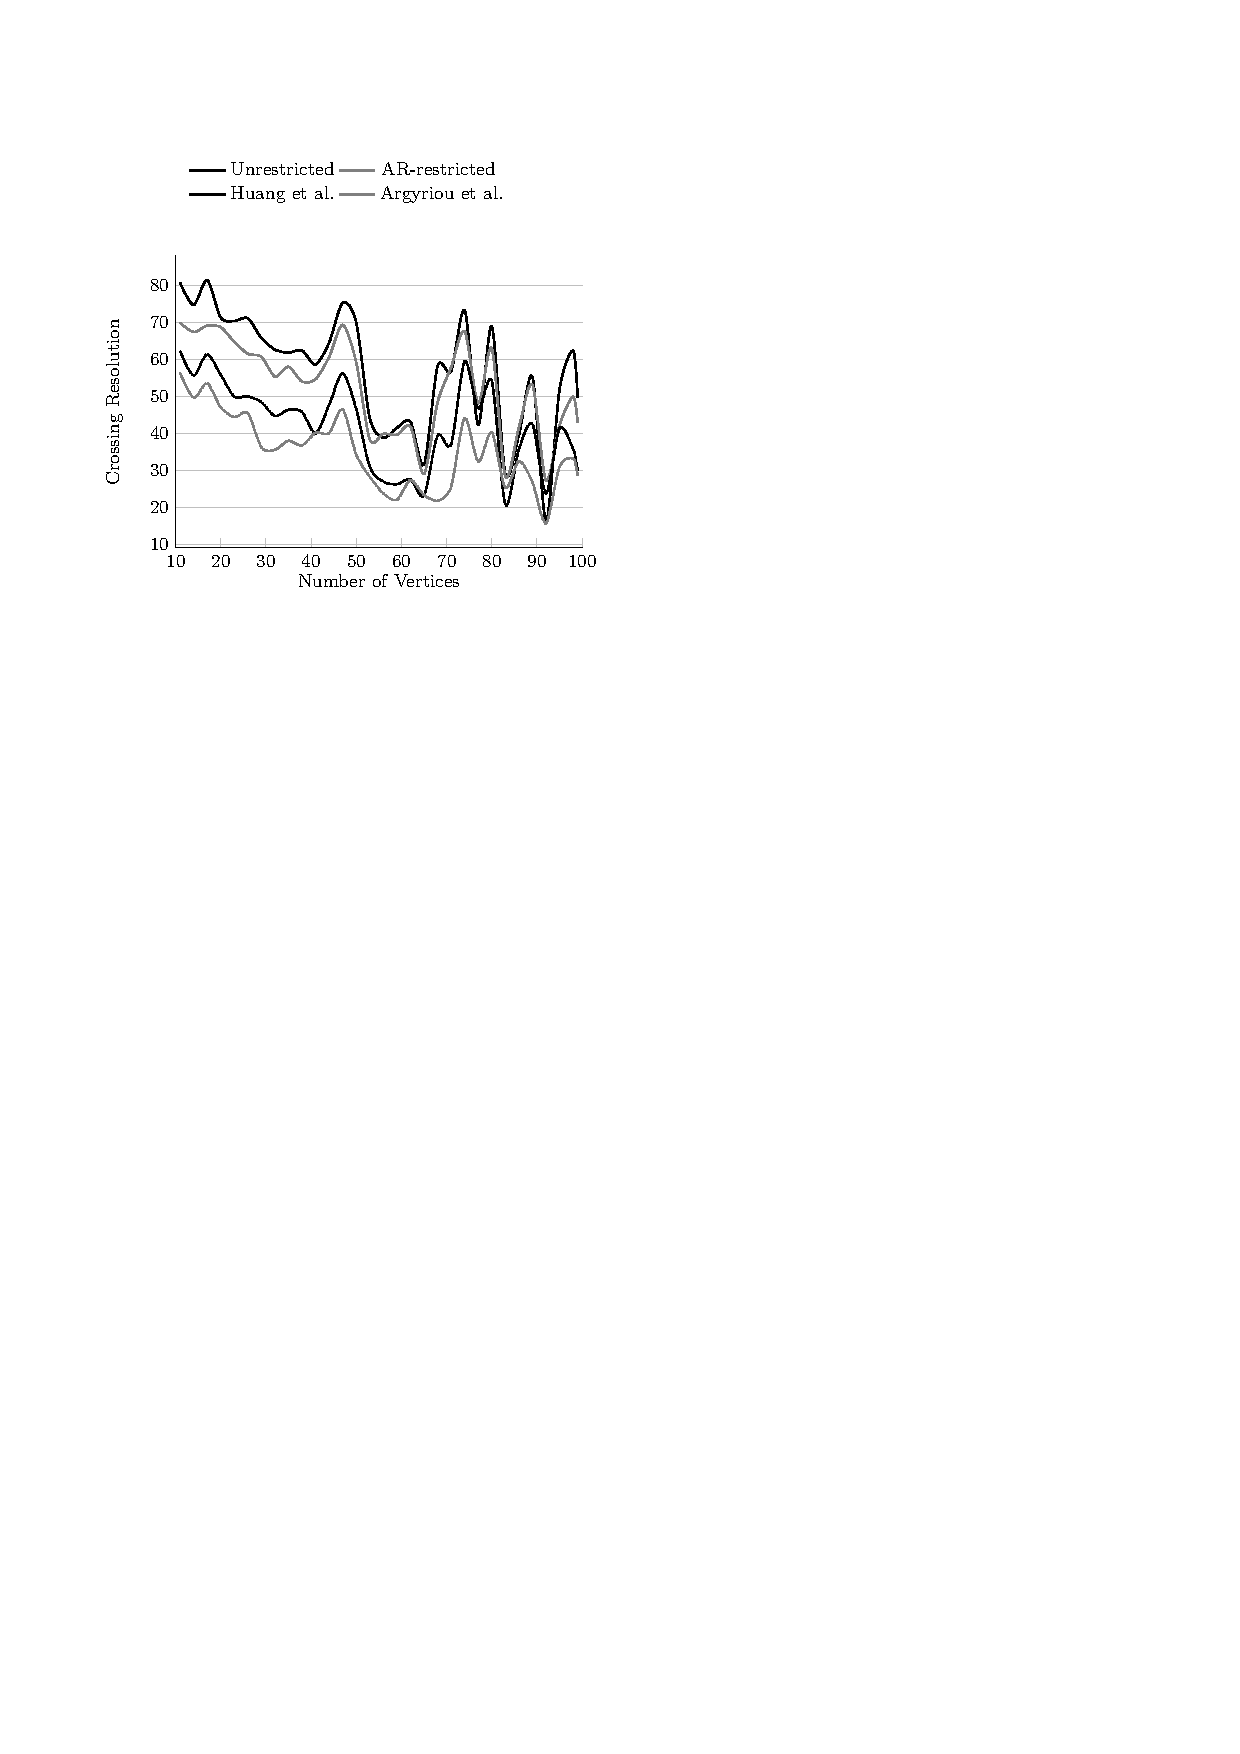
\includegraphics[scale=0.99,page=1]{figures/north}}
	\hfil
	\subfloat[\label{fig:northCrossing-2}{Aspect ratio vs no.~of vertices}]{
	\includegraphics[scale=0.99,page=2]{figures/north}}
	
	\subfloat[\label{fig:northCrossing-3}{No.~of crossings vs no.~of vertices}]{
	\includegraphics[scale=0.99,page=3]{figures/north}}
	\hfil
	\subfloat[\label{fig:northCrossing-4}{No.~of iterations vs no.~of vertices}]{
	\includegraphics[scale=0.99,page=4]{figures/north}}
	\caption{Experimental results for the crossing resolution on the AT\&T graphs.}
	\label{fig:northCrossing}
\end{figure*}

% ==================================================================
%\begin{figure*}[t!]
\centering
\subfloat[\label{fig:northTotal-1}{Total resolution vs no.~of vertices}]{
\centering
%======================
% Total Resolution
%======================
\begin{tikzpicture}
\begin{axis}[
axis x line*=bottom,xlabel style={yshift=0.2cm},ylabel style={yshift=-0.2cm},axis y line*=left,
legend style={at={(0.425,1.35)},anchor=north,,legend columns=2,draw=none},
width=0.475\textwidth,
cycle list name=mylist,
mark repeat={5},xlabel={Number of Vertices},ylabel={Total Resolution},
xtick={10,20,30,40,50,60,70,80,90,100},
xmin=10,
xmax=100,
ytick={10,20,30,40,50,60,70,80,90},
tick pos=left,ymajorgrids]
\addplot table [x=avg, y=tr rm, col sep=semicolon]{totalResolutionNorth.csv};
\addplot table [x=avg, y=tr rm-1, col sep=semicolon] {totalResolutionNorth.csv};
\addplot table [x=avg, y=tr fa, col sep=semicolon]{totalResolutionNorth.csv};
\addplot table [x=avg, y=tr tr, col sep=semicolon] {totalResolutionNorth.csv};
\legend{{Unrestricted},{AR-restricted~~},{Huang et al.},{Argyriou et al.}}
\end{axis}
\end{tikzpicture}}
\subfloat[\label{fig:northTotal-2}{Aspect ratio vs no.~of vertices}]{
\centering
%===================================
% Total Resolution Aspect Ratio
%===================================
\begin{tikzpicture}
\begin{axis}[axis x line*=bottom,xlabel style={yshift=0.2cm},axis y line*=left,legend style={at={(0.425,1.35)},
anchor=north,legend columns=2,draw=none},ylabel style={yshift=-0.2cm}, width=0.475\textwidth,cycle list name=mylist, mark repeat={5},xtick={0,10,20,30,40,50,60,70,80,90,100},ylabel={Aspect Ratio},
xlabel={Number of Vertices},
xmin=10,
xmax=100,
ytick={1,2,5,10,20,50,100,200},ymode=log, log ticks with fixed point,tick pos=left, ymajorgrids,]
\addplot table [x=avg, y=ar rm, col sep=semicolon]{totalResolutionNorth.csv};
\addplot table [x=avg, y=ar rm-1, col sep=semicolon] {totalResolutionNorth.csv};
\addplot table [x=avg, y=ar fa, col sep=semicolon]{totalResolutionNorth.csv};
\addplot table [x=avg, y=ar tr, col sep=semicolon] {totalResolutionNorth.csv};
\legend{{Unrestricted},{AR-restricted~~},{Huang et al.},{Argyriou et al.}}
\end{axis}
\end{tikzpicture}}

\subfloat[\label{fig:northTotal-3}{No.~of crossings vs no.~of vertices}]{
\centering
%======================================
% Total Resolution Crossing Number
%======================================
\begin{tikzpicture}
\begin{axis}[axis x line*=bottom,xlabel style={yshift=0.2cm},axis y line*=left,legend style={at={(0.425,1.35)},
anchor=north,legend columns=2,draw=none}, width=0.475\textwidth,cycle list name=mylist,  mark repeat={5},xtick={10,20,30,40,50,60,70,80,90,100},
xmin=10,
xmax=100,
ytick={0,250,500,750,1000,1250,1500,1750},ylabel={Number of Crossings},
xlabel={Number of Vertices},tick pos=left,ylabel style={yshift=-0.2cm}, ymajorgrids]
\addplot table [x=avg, y=cn rm, col sep=semicolon]{totalResolutionNorth.csv};
\addplot table [x=avg, y=cn rm-1, col sep=semicolon] {totalResolutionNorth.csv};
\addplot table [x=avg, y=cn fa, col sep=semicolon]{totalResolutionNorth.csv};
\addplot table [x=avg, y=cn tr, col sep=semicolon] {totalResolutionNorth.csv};
\legend{{Unrestricted},{AR-restricted~~},{Huang et al.},{Argyriou et al.}}
\end{axis}
\end{tikzpicture}}
\subfloat[\label{fig:northTotal-4}{Iterations vs no.~of vertices}]{
\centering
%==================================
% Total Resolution Iterations
%==================================
\begin{tikzpicture}
\begin{axis}[axis x line*=bottom,xlabel style={yshift=0.2cm},ylabel style={yshift=-0.2cm},axis y line*=left,legend style={at={(0.425,1.35)},
anchor=north,legend columns=2,draw=none}, width=0.475\textwidth,cycle list name=mylist, mark repeat={5},xtick={10,20,30,40,50,60,70,80,90,100},
xmin=10,
xmax=100,
ytick={0,1000,2000,3000,4000,5000,6000,7000,8000},tick pos=left,
ylabel={Iterations},
xlabel={Number of Vertices},ymajorgrids]
\addplot table [x=avg, y=it rm, col sep=semicolon]{totalResolutionNorth.csv};
\addplot table [x=avg, y=it rm-1, col sep=semicolon] {totalResolutionNorth.csv};
\addplot table [x=avg, y=it fa, col sep=semicolon]{totalResolutionNorth.csv};
\addplot table [x=avg, y=it tr, col sep=semicolon] {totalResolutionNorth.csv};
\legend{{Unrestricted},{AR-restricted~~},{Huang et al.},{Argyriou et al.}}
\end{axis}
\end{tikzpicture}}
\caption{Experimental results for the total resolution on the AT\&T graphs.}
\label{fig:northTotal}
\end{figure*}
% ==================================================================
\begin{figure*}[t!]
	\centering
	\subfloat[\label{fig:northTotal-1}{Crossing resolution vs no.~of vertices}]{
	\includegraphics[scale=0.99,page=5]{figures/north}}
	\hfil
	\subfloat[\label{fig:northTotal-2}{Aspect ratio vs no.~of vertices}]{
	\includegraphics[scale=0.99,page=6]{figures/north}}
	
	\subfloat[\label{fig:northTotal-3}{No.~of crossings vs no.~of vertices}]{
	\includegraphics[scale=0.99,page=7]{figures/north}}
	\hfil
	\subfloat[\label{fig:northTotal-4}{No.~of iterations vs no.~of vertices}]{
	\includegraphics[scale=0.99,page=8]{figures/north}}
	\caption{Experimental results for the total resolution on the AT\&T graphs.}
	\label{fig:northTotal}
\end{figure*}

% ==================================================================
%\begin{figure*}[t!]
\centering
\subfloat[\label{fig:northAngular-1}{Angular resolution vs no.~of vertices}]{
\centering
\scalebox{.95}{
\centering
%======================
% Angular Resolution
%======================
\begin{tikzpicture}
\begin{axis}[
axis x line*=bottom,xlabel style={yshift=0.2cm},ylabel style={yshift=-0.2cm},axis y line*=left,
legend style={at={(0.425,1.35)},anchor=north,,legend columns=2,draw=none},
width=0.475\textwidth,
cycle list name=mylist,
mark repeat={5},xlabel={Number of Vertices},ylabel={Angular Resolution},
xtick={10,20,30,40,50,60,70,80,90,100},
xmin=10,
xmax=100,
ytick={10,20,30,40,50,60,70,80,90},
tick pos=left,ymajorgrids]
\addplot table [x=avg, y=an rm, col sep=semicolon]{angularResolutionNorth.csv};
\addplot table [x=avg, y=an rm-1, col sep=semicolon] {angularResolutionNorth.csv};
\addplot table [x=avg, y=an fa, col sep=semicolon]{angularResolutionNorth.csv};
\addplot table [x=avg, y=an tr, col sep=semicolon] {angularResolutionNorth.csv};
\legend{{Unrestricted},{AR-restricted~~},{Huang et al.},{Argyriou et al.}}
\end{axis}
\end{tikzpicture}}}
\subfloat[\label{fig:northAngular-2}{Aspect ratio vs no.~of vertices}]{
\centering
\scalebox{.95}{
\centering
%===================================
% Angular Resolution Aspect Ratio
%===================================
\begin{tikzpicture}
\begin{axis}[axis x line*=bottom,xlabel style={yshift=0.2cm},axis y line*=left,legend style={at={(0.425,1.35)},
anchor=north,legend columns=2,draw=none},ylabel style={yshift=-0.2cm}, width=0.475\textwidth,cycle list name=mylist, mark repeat={5},xtick={0,10,20,30,40,50,60,70,80,90,100},ylabel={Aspect Ratio},
xlabel={Number of Vertices},
xmin=10,
xmax=100,
ytick={1,2,5,10,20,50,100,200},ymode=log, log ticks with fixed point,tick pos=left, ymajorgrids,]
\addplot table [x=avg, y=ar rm, col sep=semicolon]{angularResolutionNorth.csv};
\addplot table [x=avg, y=ar rm-1, col sep=semicolon] {angularResolutionNorth.csv};
\addplot table [x=avg, y=ar fa, col sep=semicolon]{angularResolutionNorth.csv};
\addplot table [x=avg, y=ar tr, col sep=semicolon] {angularResolutionNorth.csv};
\legend{{Unrestricted},{AR-restricted~~},{Huang et al.},{Argyriou et al.}}
\end{axis}
\end{tikzpicture}}}

\subfloat[\label{fig:northAngular-3}{No.~of crossings vs no.~of vertices}]{
\centering
\scalebox{.95}{
\centering
%======================================
% Angular Resolution Crossing Number
%======================================
\begin{tikzpicture}
\begin{axis}[axis x line*=bottom,xlabel style={yshift=0.2cm},axis y line*=left,legend style={at={(0.425,1.35)},
anchor=north,legend columns=2,draw=none}, width=0.475\textwidth,cycle list name=mylist,  mark repeat={5},xtick={10,20,30,40,50,60,70,80,90,100},
xmin=10,
xmax=100,
ytick={0,250,500,750,1000,1250,1500,1750},ylabel={Number of Crossings},
xlabel={Number of Vertices},tick pos=left,ylabel style={yshift=-0.2cm}, ymajorgrids]
\addplot table [x=avg, y=cn rm, col sep=semicolon]{angularResolutionNorth.csv};
\addplot table [x=avg, y=cn rm-1, col sep=semicolon] {angularResolutionNorth.csv};
\addplot table [x=avg, y=cn fa, col sep=semicolon]{angularResolutionNorth.csv};
\addplot table [x=avg, y=cn tr, col sep=semicolon] {angularResolutionNorth.csv};
\legend{{Unrestricted},{AR-restricted~~},{Huang et al.},{Argyriou et al.}}
\end{axis}
\end{tikzpicture}}}
\subfloat[\label{fig:northAngular-4}{Iterations vs no.~of vertices}]{
\centering
\scalebox{.95}{
\centering
%==================================
% Angular Resolution Iterations
%==================================
\begin{tikzpicture}
\begin{axis}[axis x line*=bottom,xlabel style={yshift=0.2cm},ylabel style={yshift=-0.2cm},axis y line*=left,legend style={at={(0.425,1.35)},
anchor=north,legend columns=2,draw=none}, width=0.475\textwidth,cycle list name=mylist, mark repeat={5},xtick={10,20,30,40,50,60,70,80,90,100},
xmin=10,
xmax=100,
ytick={0,1000,2000,3000,4000,5000,6000,7000,8000},tick pos=left,
ylabel={Iterations},
xlabel={Number of Vertices},ymajorgrids]
\addplot table [x=avg, y=it rm, col sep=semicolon]{angularResolutionNorth.csv};
\addplot table [x=avg, y=it rm-1, col sep=semicolon] {angularResolutionNorth.csv};
\addplot table [x=avg, y=it fa, col sep=semicolon]{angularResolutionNorth.csv};
\addplot table [x=avg, y=it tr, col sep=semicolon] {angularResolutionNorth.csv};
\legend{{Unrestricted},{AR-restricted~~},{Huang et al.},{Argyriou et al.}}
\end{axis}
\end{tikzpicture}}}
\caption{Experimental results for the angular resolution on the AT\&T graphs.}
\label{fig:northAngular}
\end{figure*}
% ==================================================================
\begin{figure*}[t!]
	\centering
	\subfloat[\label{fig:northAngular-1}{Crossing resolution vs no.~of vertices}]{
	\includegraphics[scale=0.99,page=9]{figures/north}}
	\hfil
	\subfloat[\label{fig:northAngular-2}{Aspect ratio vs no.~of vertices}]{
	\includegraphics[scale=0.99,page=10]{figures/north}}
	
	\subfloat[\label{fig:northAngular-3}{No.~of crossings vs no.~of vertices}]{
	\includegraphics[scale=0.99,page=11]{figures/north}}
	\hfil
	\subfloat[\label{fig:northAngular-4}{No.~of iterations vs no.~of vertices}]{
	\includegraphics[scale=0.99,page=12]{figures/north}}
	\caption{Experimental results for the angular resolution on the AT\&T graphs.}
	\label{fig:northAngular}
\end{figure*}

% ==================================================================
\begin{figure*}[!t]
\centering
\subfloat[\label{fig:crossingResolutionGrid}{Crossing resolution vs no.~of vertices}]{
\centering
%======================
% Crossing Resolution
%======================
\begin{tikzpicture}
\begin{axis}[
axis x line*=bottom,xlabel style={yshift=0.2cm},ylabel style={yshift=-0.2cm},axis y line*=left,
legend style={at={(0.425,1.35)},anchor=north,,legend columns=2,draw=none},
width=0.475\textwidth,
cycle list name=mylist,
mark repeat={5},xlabel={Number of Vertices},ylabel={Crossing Resolution},
xtick={10,20,30,40,50,60,70,80,90,100},
xmin=10,
xmax=100,
ytick={10,20,30,40,50,60,70,80,90},
tick pos=left,ymajorgrids]
\addplot table [x=n, y=crossing resolution rm1M, col sep=semicolon]{gridExperiment.csv};
\addplot table [x=n, y=crossing resolution rm10k, col sep=semicolon] {gridExperiment.csv};
\addplot table [x=n, y=crossing resolution rm1000, col sep=semicolon]{gridExperiment.csv};
\addplot table [x=n, y=crossing resolution rm100, col sep=semicolon] {gridExperiment.csv};
\addplot table [x=n, y=crossing resolution rm, col sep=semicolon]{gridExperiment.csv};
\legend{{$10^6 \times 10^6$},{$10^4 \times 10^4$},{$10^3 \times 10^3$},{$10^2 \times 10^2$}}
\end{axis}
\end{tikzpicture}}
\subfloat[\label{fig:crossingResolutionAspectRatioGrid}{Aspect ratio vs no.~of vertices}]{
\centering
%===================================
% Crossing Resolution Aspect Ratio
%===================================
\begin{tikzpicture}
\begin{axis}[axis x line*=bottom,xlabel style={yshift=0.2cm},axis y line*=left,legend style={at={(0.425,1.35)},
anchor=north,legend columns=2,draw=none},ylabel style={yshift=-0.2cm}, width=0.475\textwidth,cycle list name=mylist, mark repeat={5},xtick={0,10,20,30,40,50,60,70,80,90,100},ylabel={Aspect Ratio},
xlabel={Number of Vertices},
xmin=10,
xmax=100,
ytick={1,2,5,10,20,50,100,200},ymode=log, log ticks with fixed point,tick pos=left, ymajorgrids,]
\addplot table [x=n, y=Aspect ratio rm1M, col sep=semicolon]{gridExperiment.csv};
\addplot table [x=n, y=Aspect ratio rm10k, col sep=semicolon] {gridExperiment.csv};
\addplot table [x=n, y=Aspect ratio rm1000, col sep=semicolon]{gridExperiment.csv};
\addplot table [x=n, y=Aspect ratio rm100, col sep=semicolon] {gridExperiment.csv};
\addplot table [x=n, y=Aspect ratio rm, col sep=semicolon]{gridExperiment.csv};
\legend{{$10^6 \times 10^6$},{$10^4 \times 10^4$},{$10^3 \times 10^3$},{$10^2 \times 10^2$}}
\end{axis}
\end{tikzpicture}}

\subfloat[\label{fig:crossingResolutionCrossingNumberGrid}{No.~of crossings vs no.~of vertices}]{
\centering
%======================================
% Crossing Resolution Crossing Number
%======================================
\begin{tikzpicture}
\begin{axis}[axis x line*=bottom,xlabel style={yshift=0.2cm},axis y line*=left,legend style={at={(0.425,1.35)},
anchor=north,legend columns=2,draw=none}, width=0.475\textwidth,cycle list name=mylist,  mark repeat={5},xtick={10,20,30,40,50,60,70,80,90,100},
xmin=10,
xmax=100,
ytick={0,250,500,750,1000,1250,1500,1750},ylabel={Number of Crossings},
xlabel={Number of Vertices},tick pos=left,ylabel style={yshift=-0.2cm}, ymajorgrids]
\addplot table [x=n, y=Crossing number rm1M, col sep=semicolon]{gridExperiment.csv};
\addplot table [x=n, y=Crossing number rm10k, col sep=semicolon] {gridExperiment.csv};
\addplot table [x=n, y=Crossing number rm1000, col sep=semicolon]{gridExperiment.csv};
\addplot table [x=n, y=Crossing number rm100, col sep=semicolon] {gridExperiment.csv};
\addplot table [x=n, y=Crossing number rm, col sep=semicolon] {gridExperiment.csv};
\legend{{$10^6 \times 10^6$},{$10^4 \times 10^4$},{$10^3 \times 10^3$},{$10^2 \times 10^2$}}
\end{axis}
\end{tikzpicture}}
\subfloat[\label{fig:crossingResolutionTimeGrid}{Iterations vs no.~of vertices}]{
\centering
%==================================
% Crossing Resolution Iterations
%==================================
\begin{tikzpicture}
\begin{axis}[axis x line*=bottom,xlabel style={yshift=0.2cm},ylabel style={yshift=-0.2cm},axis y line*=left,legend style={at={(0.425,1.35)},
anchor=north,legend columns=2,draw=none}, width=0.475\textwidth,cycle list name=mylist, mark repeat={5},xtick={10,20,30,40,50,60,70,80,90,100},
xmin=10,
xmax=100,
ytick={0,1000,2000,3000,4000,5000,6000,7000,8000},tick pos=left,
ylabel={Iterations},
xlabel={Number of Vertices},ymajorgrids]
\addplot table [x=n, y=Iterations rm1M, col sep=semicolon]{gridExperiment.csv};
\addplot table [x=n, y=Iterations rm10k, col sep=semicolon] {gridExperiment.csv};
\addplot table [x=n, y=Iterations rm1000, col sep=semicolon]{gridExperiment.csv};
\addplot table [x=n, y=Iterations rm100, col sep=semicolon] {gridExperiment.csv};
\addplot table [x=n, y=Iterations rm, col sep=semicolon] {gridExperiment.csv};
\legend{{$10^6 \times 10^6$},{$10^4 \times 10^4$},{$10^3 \times 10^3$},{$10^2 \times 10^2$}}
\end{axis}
\end{tikzpicture}}
\caption{Our experimental results on the crossing resolution with different grid restrictions.
The double line corresponds to our unrestricted algorithm.}
\label{fig:experimentsGrid}
\end{figure*}
% ==================================================================

\begin{table*}
\caption{Summary of the results for the Graph Drawing Contest 2017.}
\centering
\begin{tabular}{c|c|c|c|c}
\toprule
\rowcolor{gray!30!}~~Graph~~ & ~~CoffeeVM~~ & ~~T\"ubingenMidnight~~ & ~~Time restricted~~ & ~~Our best~~ \\
\midrule
\rowcolor{gray!30!} 1  & 90$^\circ$  & 77$^\circ$ & 90$^\circ$ & 90$^\circ$\\
\rowcolor{gray!00!} 2  & 88$^\circ$  & 42$^\circ$ & 88$^\circ$ & 89$^\circ$\\
\rowcolor{gray!30!} 3  & 90$^\circ$  & 89$^\circ$ & 88$^\circ$ & 90$^\circ$\\
\rowcolor{gray!00!} 4  & 89$^\circ$  & 89$^\circ$ & 77$^\circ$ & 89$^\circ$\\
\rowcolor{gray!30!} 5  & 80$^\circ$  & 30$^\circ$ & 79$^\circ$ & 87$^\circ$\\
\rowcolor{gray!00!} 6  & 90$^\circ$  & 78$^\circ$ & 90$^\circ$ & 90$^\circ$\\
\rowcolor{gray!30!} 7  & 57$^\circ$  & 34$^\circ$ & 56$^\circ$ & 64$^\circ$\\
\rowcolor{gray!00!} 8  & 85$^\circ$  & 61$^\circ$ & 81$^\circ$ & 89$^\circ$\\
\rowcolor{gray!30!} 9  & 60$^\circ$  & 9$^\circ$  & 55$^\circ$ & 88$^\circ$\\
\rowcolor{gray!00!} 10 & 21$^\circ$  & 4$^\circ$  & 24$^\circ$ & 24$^\circ$\\
\rowcolor{gray!30!} 11 & 47$^\circ$  & 6$^\circ$  & 57$^\circ$ & 72$^\circ$\\
\rowcolor{gray!00!} 12 & 36$^\circ$  & 5$^\circ$  & 26$^\circ$ & 36$^\circ$\\
\rowcolor{gray!30!} 13 & 25$^\circ$  & 4$^\circ$  & 22$^\circ$ & 34$^\circ$\\
\rowcolor{gray!00!} 14 & 34$^\circ$  & 5$^\circ$  & 30$^\circ$ & 43$^\circ$\\
\rowcolor{gray!30!} 15 & 21$^\circ$  & 4$^\circ$  & 13$^\circ$ & 29$^\circ$\\
\rowcolor{gray!00!} 16 & 20$^\circ$  & 3$^\circ$  & 12$^\circ$ & 26$^\circ$\\
\bottomrule
\end{tabular}
\label{tab:gdContest2017}
\end{table*}

While our unrestricted algorithm produces drawings with better crossing resolution, this comes at a cost of drastically increased aspect ratio (see Fig.~\ref{fig:cr-res-2}), which, however, is still better that the corresponding aspect ratio of the drawings produced by the algorithm of Argyriou et al. For the latter algorithm, it seems that the forces due to the angles formed at the crossings outperform the corresponding spring forces, which try to keep the lengths of the edges short. Going back to our unrestricted algorithm, its behavior is up to a certain degree expected, mainly due to the fact that there is no control on the lengths of the edges (as it is, e.g., in the case of the force-directed algorithm of Huang et al.~\cite{DBLP:journals/vlc/HuangEHL13}, whose sping forces inpose stong restrictions on the edge lengths). On the other hand, the restricted variant of our algorithm, which does not allow the aspect ratio to increase, has more or less comparable performance (in terms of aspect ratio) as the one of Huang et al.

Regarding the number of crossings, the restricted variant of our algorithm and the force-directed algorithm of Huang et al.\ yield drawings with comparable number of crossings, which at the same time is significantly smaller than the  number of crossings produced by the two other algorithms; see Fig.~\ref{fig:cr-res-3}.

A different behavior can be observed in the number of iterations, which are required by the algorithms to converge; refer to Fig.~\ref{fig:cr-res-4}. We note here that we used different criteria to determine whether the algorithms of our experiment had converged. For our algorithms and for the force-directed algorithm by Huang et al., we assumed that the algorithm had converged, if the crossing resolution between 500 consecutive iterations was not improved by more than 0.001 degrees. For the algorithm by Argyriou et al., we decided to use a much more restricted convergence criterion, because the produced layouts can change vastly between  consecutive iterations. We made this choice mainly to have ``comparable'' number of iterations among the algorithms of the experiment. In this direction, we adopted the convergence criterion that the authors used in their previous experimental analysis, that is, we assumed that the algorithm had converged, if the crossing resolution between two consecutive iterations was not improved by more than 0.001 degrees. Observe that even under this different convergence criterion, the algorithm needs significantly more iterations to converge than the remaining three algorithms of the experiment; see Fig.~\ref{fig:cr-res-4}. 

The maximum number of iterations that each of the algorithms of the experiment could perform in order to converge was set to 100.000, but notably this limit was never reached. 

We observe that both force-directed algorithms by Argyriou et al.\ and by Huang et al.\ seem to require a great amount of iterations to converge for small graphs, where a drawing with really good crossing resolution is more likely to be computed. However, that for larger graphs the algorithm by Huang et al.\ requires the least amount of iterations. Regarding the unrestricted and the restricted variants of our algorithm, it is clear that both require comparable number of iterations to converge, but clearly more than the ones of the algorithm by Huang et al.

\myparagraph{Total resolution} Our results for the total resolution are summarized in Fig.~\ref{fig:to-res}. Here, each algorithm was adjusted to maximize both the crossing and the angular resolution, simultaneously. For the vast majority of the graphs in the experiment, both our unrestricted algorithm and its restricted variant yield drawings with better total resolution than the corresponding ones by Argyriou et al. The drawings produced by the algorithm by Huang et al.\ seems to have worse total resolution; see Fig.~\ref{fig:to-res-1}. Note, however, that both variants of our algorithm as well as the force-directed algorithm by Argyriou et al.\ tend to produce drawings of the same total resolution for larger graphs with a small difference in our favor.

Contrary to the results for the total resolution, the results for the aspect ratio show that the drawings produced by the algorithm by Huang et al.\ are better (in terms of this measure) than the drawings produced by remaining algorithms; see Fig.~\ref{fig:to-res-2}. 
%More concretely, the 
The drawings produced by the restricted variant of our algorithm have slightly worse aspect ratios. Then, the ones produced by the force-directed algorithm by Argyriou et al.\ follow. Again, we observe that our unrestricted algorithm leads to drawings with very high aspect ratio.

Analogous observations can be made for the number of crossings of the produced layouts; see Fig.~\ref{fig:to-res-3}. The restricted variant of our algorithm and the algorithm by Huang et al.\ yield drawings with the least number of crossings. Comparable but slightly worse (in terms of the number of crossings) are the drawings produced by the force-directed algorithm by Argyriou et al. Our unrestricted algorithm requires the largest number of crossings, which turns out to be notably higher than the corresponding ones of the other three algorithms.

On the negative side, both the unrestricted and the restricted variants of our algorithm require more iterations than the force-directed algorithm by Huang et al.\ in order to converge; see Fig.~\ref{fig:to-res-4}. Recall, however, that the latter algorithm is clearly outperformed by both our variants in term of total resolution. The algorithm by Argyriou et al.\ clearly requires the highest number of iterations (especially for large graphs). We note that the convergence criterion was the same as for the crossing resolution; however, the measured quality was (not the crossing but) the total resolution.

\myparagraph{Angular resolution} We conclude the analysis of our experimental evaluation with the results for the angular resolution; see Fig.~\ref{fig:an-res}. Here, each algorithm was adjusted  to maximize only the angular resolution (i.e., by ignoring the drawing's crossing resolution). A notable observation is that, for small graphs the best results are achieved by the algorithm by Argyriou et al., while for medium-size graphs by our unrestricted algorithm; see Fig.~\ref{fig:an-res-1}. For large graphs, the two algorithms tend to have the same performance. The restricted variant of our algorithm yields drawings with slightly worse angular resolution. The algorithm by Huang et al.\ is outperformed by all algorithms of the experiment.

The results for the aspect ratio, the number of crossings and the required number of iterations are very similar with corresponding ones for the total resolution; see Figs.~\ref{fig:an-res-2}--\ref{fig:an-res-4}. This observation suggests that, for most of the graphs of our experiment, the angular resolution dominates the crossing resolution (and thus is the one defining the total resolution) in the constructed drawings, which explains the similarity in the reported results. The small differences result from the fact that the crossing resolution cannot be entirely neglected.

% ==================================================================
\subsection{The AT\&T  Graph Test Set}
\label{ssec:north}
% ==================================================================

In this subsection, we report the results of our experimental evaluation for the non-planar AT\&T graphs. Note that again we did not impose any grid constraint on our algorithms. The corresponding results are illustrated in Figs.~\ref{fig:northCrossing}, \ref{fig:northTotal} and~\ref{fig:northAngular}. In general, we observed that the variance of the results is much larger than in the experiments on the Rome graphs. This manifests in spikes of large magnitude in the illustrations of the results indicates that the structural properties of the graphs in this second test set varies vastly between graphs of different sizes.

\myparagraph{Crossing resolution} As with the Rome graphs, we observed again that both variants of our algorithm again outperformed the two force-directed algorithms; see Fig.~\ref{fig:northCrossing-1}. Remarkable is the synchronous behavior of all four algorithms regarding the crossing resolution, as the curves are nearly parallel. The results actually indicate that one can classify these graphs into ``hard'' and ``easy'' ones, when maximizing their crossing resolution. In particular, the graphs with 50 to 70 vertices appear to be harder than the graphs with 70 to 80 vertices. As expected, the aspect ratio of the drawings produced by both the unrestricted and the restricted variants of our algorithm depends vastly on the number of vertices of the graphs. However, this natural behavior cannot be observed in the resulting drawings of the two force-directed algorithms, which appear to be quite unstable resulting in a large variance. Again the restricted variant of our algorithm and the two force-directed algorithms produce drawings with similar aspect ratio, which is much lower than the one of our unrestricted algorithm for larger graphs. All four algorithms behave nearly the same in terms of the number of crossings; see Fig.~\ref{fig:northCrossing-3}. In terms of the number of iterations need for convergence, we observe that somewhat surprisingly the algorithm of Argyriou et al.\ converges using the least amount of iterations, while the remaining three algorithms behave nearly the same; see Fig.~\ref{fig:northCrossing-4}.

\myparagraph{Total resolution} For small graphs, we observed similar results as in the experiment on the Rome graphs, that is, our unrestricted algorithm outperforms (in terms of the total resolution) the other three algorithms of the experiment, while the restricted variant of our algorithm is slightly better than the algorithms by Argyriou et al.\ and by Huang et al.; see Fig.~\ref{fig:northTotal-1}. For larger graphs, however, the two variants of our algorithm achieve similar results, while still outperforming the algorithm by Huang et al. Regarding the aspect ratio and the number of crossings of the produced drawings, we observe that all algorithms have more or less the same behavior as when adjusted for maximizing the crossing resolution only. The only exception can be observed in the algorithm by Huang et al., which performs more stable; see Figs.~\ref{fig:northTotal-2} and~\ref{fig:northTotal-3}. With respect to the number of iterations required for convergence, the two variants of our algorithms and the force-directed algorithm by Argyriou et al.\ show similar behavior. The algorithm by Huang et al., on the other hand, needs less iterations for convergence; see Fig.~\ref{fig:northTotal-4}. Note, however, that there is no immediate correlation with the number of vertices of the graph.


\myparagraph{Angular resolution} Here, the picture is not so clear concerning the ranking of the algorithms; see Fig.~\ref{fig:northAngular-1}. Only the algorithm by Huang et al.\ seems to be mostly at last in the rank. Concerning the aspect ratio, we see very good behavior for the restricted variant of our algorithm and the algorithm by Huang et al., while the remaining two algorithms show large variance and much worse values; see Fig.~\ref{fig:northAngular-2}. Regarding the number of crossings, we again observe that all algorithms have similar behavior. Note, however, that the unrestricted variant of our algorithm and the algorithm by Argyriou et al.\ yield drawings with more crossing, especially for graphs with large number of vertices; see Fig.~\ref{fig:northAngular-3}. Finally, both variants of our algorithm and the force-directed algorithm by Huang et al.\ need comparable number of iterations for convergence, which most of the times is lower than the corresponding one by Argyriou et al.; see Fig.~\ref{fig:northAngular-4}.

Summarizing, we conclude that compared to the Rome graphs, the AT\&T graphs show a much higher variance regarding the various resolution measures. %The crossing resolution results of our method still outperform the other approaches by far but especially for larger graphs as well as angular and total resolution the methods tend to perform similarly.

% ==================================================================
\subsection{Grid Restricted Drawings}
\label{ssec:grid}
% ==================================================================

In addition to the experiments that we have described so far, we also evaluated how our algorithm performs, if we restrict its vertices to integer grid coordinates. In particular, we were interesting to see how the different quality measures that we have investigated so far are affected by the restrictions imposed on having the vertices of the graph on integer grids of different sizes:

\begin{enumerate}[(i)]
\item $10^6 \times 10^6$
\item $10^4 \times 10^4$
\item $10^3 \times 10^3$, and
\item $10^2 \times 10^2$.
\end{enumerate}

The test suite for this experiment was the non-planar Rome graphs. The algorithm to be evaluated was the variant of our algorithm that optimizes the drawing's crossing resolution (without any restriction on the aspect ratio). However, since this algorithm is guaranteed to produce a grid drawing, only if its initial drawing is grid, each of the Rome graphs was initially laid out by randomly placing its vertices on the underlying grid, ensuring that neither two vertices nor two edges overlap. Fig.~\ref{fig:experimentsGrid} summarizes the results.

Regarding the crossing resolution, we natural observe that the bigger the grid is, the easier it is to compute a drawing with high crossing resolution; see Fig.~\ref{fig:crossingResolutionGrid}. More precisely, the grid of size $10^2 \times 10^2$ was too restrictive for the vast majority of the graphs. As a result, the reported drawings were often the initial ones (as our algorithm could not improve them), especially for large graphs. Significantly fewer were the graphs for which our algorithm could not report an improved drawing, when the underlying grid was of size $10^3 \times 10^3$. The crossing resolution of the drawings produced by our algorithm, when the underlying grid was of size $10^4 \times 10^4$, were on average worse by only $10^\circ$ than those produced by our algorithm, when imposing no restriction on the size of the underlying grid (refer to the double line in Fig.~\ref{fig:crossingResolutionGrid}). As expected, the gap was more narrow, when the underlying grid was of size $10^6 \times 10^6$.

The aspect ratio of the computed drawings was more or less the same regardless of the size of the underlying grid, with the exception of the drawings computed on the $10^2 \times 10^2$ grid; see Fig.~\ref{fig:crossingResolutionAspectRatioGrid}. The fact that the aspect ratio of these drawings was worse can be explained of course by the fact that in most cases an improved drawing could not be reported.

As expected, the smaller the underlying grid is, the more crossings the computed drawings contain; see Fig.~\ref{fig:crossingResolutionCrossingNumberGrid}. As a result, the drawings produced by our algorithm, when imposing no restriction on the size of the underlying grid, are clearly better (in terms of the number of crossings) than those produced by our algorithm, when the size of the underlying grid is limited. As a matter of fact, the larger the underlying grid is, the fewer crossing the reported drawings have, and the differences are quite clear. Exceptional are the grids of sizes $10^4 \times 10^4$ and $10^6 \times 10^6$, where the improvement (in the number of crossings) from the latter to the former is small on average; this can partially be explained by the different choices of the initial drawings.

In general, the number of iterations needed for convergence increases with the size of the underlying grid; see Fig.~\ref{fig:crossingResolutionTimeGrid}. Exceptional seems to be the $10^2 \times 10^2$ grid, which verifies our previous observation that for the vast majority of the graphs an improved drawing could not be reported.

In conclusion, we can state that our algorithm is still able to compute drawings with high crossing resolution, when restricted to a grid, as long as the grid is not too small. However, the computation of a grid drawing takes longer, which is of course expected. Finally, the choice of the initial grid drawing seems to affect the performance of our algorithm, both with respect to the quality of the produced drawings (counted here in terms of the crossing resolution), but also with respect to the number of iterations needed for convergence.

% ==================================================================
\subsection{Graph Drawing Contests 2018 and 2019}
\label{ssec:contest}
% ==================================================================

\begin{table*}
\caption{Summary of the results for the Graph Drawing Contest 2018.}
\centering
\begin{tabular}{c|c|c|c}
\toprule
\rowcolor{gray!30!} ~~Graph~~ & ~~T\"ubingenColdShower~~ & ~~CoffeeVM+~~ & ~~Our best~~ \\
\midrule
\rowcolor{gray!30!} 1  & 87$^\circ$ & 58$^\circ$ & 89.99$^\circ$\\
\rowcolor{gray!00!} 2  & 90$^\circ$ & 90$^\circ$ & 88.70$^\circ$\\
\rowcolor{gray!30!} 3  & 88$^\circ$ & 85$^\circ$ & 89.95$^\circ$\\
\rowcolor{gray!00!} 4  & 88$^\circ$ & 60$^\circ$ & 89.05$^\circ$\\
\rowcolor{gray!30!} 5  & 71$^\circ$ & 48$^\circ$ & 86.96$^\circ$\\
\rowcolor{gray!00!} 6  & 89$^\circ$ & 71$^\circ$ & 89.96$^\circ$\\
\rowcolor{gray!30!} 7  & 80$^\circ$ & 43$^\circ$ & 63.62$^\circ$\\
\rowcolor{gray!00!} 8  & 34$^\circ$ & 27$^\circ$ & 89.28$^\circ$\\
\rowcolor{gray!30!} 9  & 77$^\circ$ & 60$^\circ$ & 88.20$^\circ$\\
\rowcolor{gray!00!} 10 & 13$^\circ$ & 19$^\circ$ & 23.72$^\circ$\\
\rowcolor{gray!30!} 11 & 11$^\circ$ & 22$^\circ$ & 72.00$^\circ$\\
\rowcolor{gray!00!} 12 & 74$^\circ$ &  9$^\circ$ & 35.86$^\circ$\\
\rowcolor{gray!30!} 13 &  2$^\circ$ &  2$^\circ$ & 33.68$^\circ$\\
\rowcolor{gray!00!} 14 &  3$^\circ$ & 11$^\circ$ & 43.08$^\circ$\\
\bottomrule
\end{tabular}
\label{tab:gdContest2018}
\end{table*}

Every year, the Graph Drawing conference organizes a contest, in which the task is to visualize a set of challenge graphs in a predefined drawing style. The teams participating to the contest receive a set of challenge graphs, and after one hour they must submit their final drawings for each of them. The team with the highest cumulative score wins. In years 2017 and 2018, the task of the contest was to produce a drawing for each of the given challenge graphs with as high crossing resolution as possible (which actually also formed our primary motivation for this work). 

\myparagraph{Graph Drawing Contest 2017} In 2017, we participated to the contest (by implementing a mixture of the two force-directed algorithms by Argyriou et al. and by Huang et al.). 
%
Table~\ref{tab:gdContest2017} summarizes the results, which are also available at \texttt{www.graphdrawing.de/contest2017/results.html}. 

It is far from clear that the wining team was the team  ``\texttt{CoffeeVM}''. Our team ``\texttt{TuebingenMidnight}''  miserably performed; we actually took the third position out of a total of four teams that participated. As already mentioned, each team had only one hour to compute a layout for each of the challenge graphs, which in year 2017 were in total $16$. In Table~\ref{tab:gdContest2017}, we additionally provide results that were achieved by the algorithm presented in this paper in two settings; within the time limit of the contest (see column ``Time restricted''), as well as our best results, which were achieved without any time limitations (see column ``Our best'').

We can observe that for almost all graphs, our new approach achieves only slightly worse results than the ones of the contest's winner when restricted within the one hour. On a few graphs (namely, graphs 10 and 11), we even achieved better results. With a single exception (namely, graph 4), we could easily outperform the results that we achieved with the spring-embedder algorithm. If we neglect the time restriction, then for all the graphs, the results  are (sometimes considerably) better than or at least about the same as the contest's winner. 

\myparagraph{Graph Drawing Contest 2018} In 2018, we participated again to the Graph Drawing contest under the name ``\texttt{T\"ubingenColdShower}'' (using an implementation of the algorithm presented in this paper). The winning team of the Graph Drawing contest 2017 also participated under the name ``\texttt{CoffeeVM+}''. Table~\ref{tab:gdContest2018} summarizes the results, which are also available at \texttt{www.graphdrawing.de/contest2018/results.html}. 

It is eye-catching that our team was the winning one; team \texttt{CoffeeVM+} took the second position of the contest (out of a total of four teams that participated to the contest). It is worth noting that for almost all $14$ challenge graphs our team achieved significantly better results than those of the second team \texttt{CoffeeVM+}, which clearly indicates that our new approach is very competitive (and definitely better than our previous,  as also evidenced by the experimental evaluation).



\section{Sample Drawings}
\label{app:samples}

In this section, we present sample drawings of the 5th and of the 9th graph given in the Graph Drawing contest 2017 that are produced by different variants of our algorithm and of the algorithms by Argyriou et al.~\cite{DBLP:journals/cj/ArgyriouBS13}, and by Huang et al.~\cite{DBLP:journals/vlc/HuangEHL13}; see Figures~\ref{fig:graph5} and~\ref{fig:graph9}, respectively. Each variant was obtained by adjusting each of the aforementioned algorithms to optimize the crossing resolution, the angular resolution and the total resolution, respectively; the aesthetic criterion optimized by each variant is reported in the caption of its corresponding subfigure. As initial drawings for all algorithms, we used the layouts shown in Fig.~\ref{fig:graph5And9-yfiles} that we computed with the SmartOrganic layouter of the yFiles library~\cite{DBLP:books/sp/04/WieseE004}.

\begin{figure}[t]
\centering
\subfloat[\label{fig:graph5-yfiles}{}]{
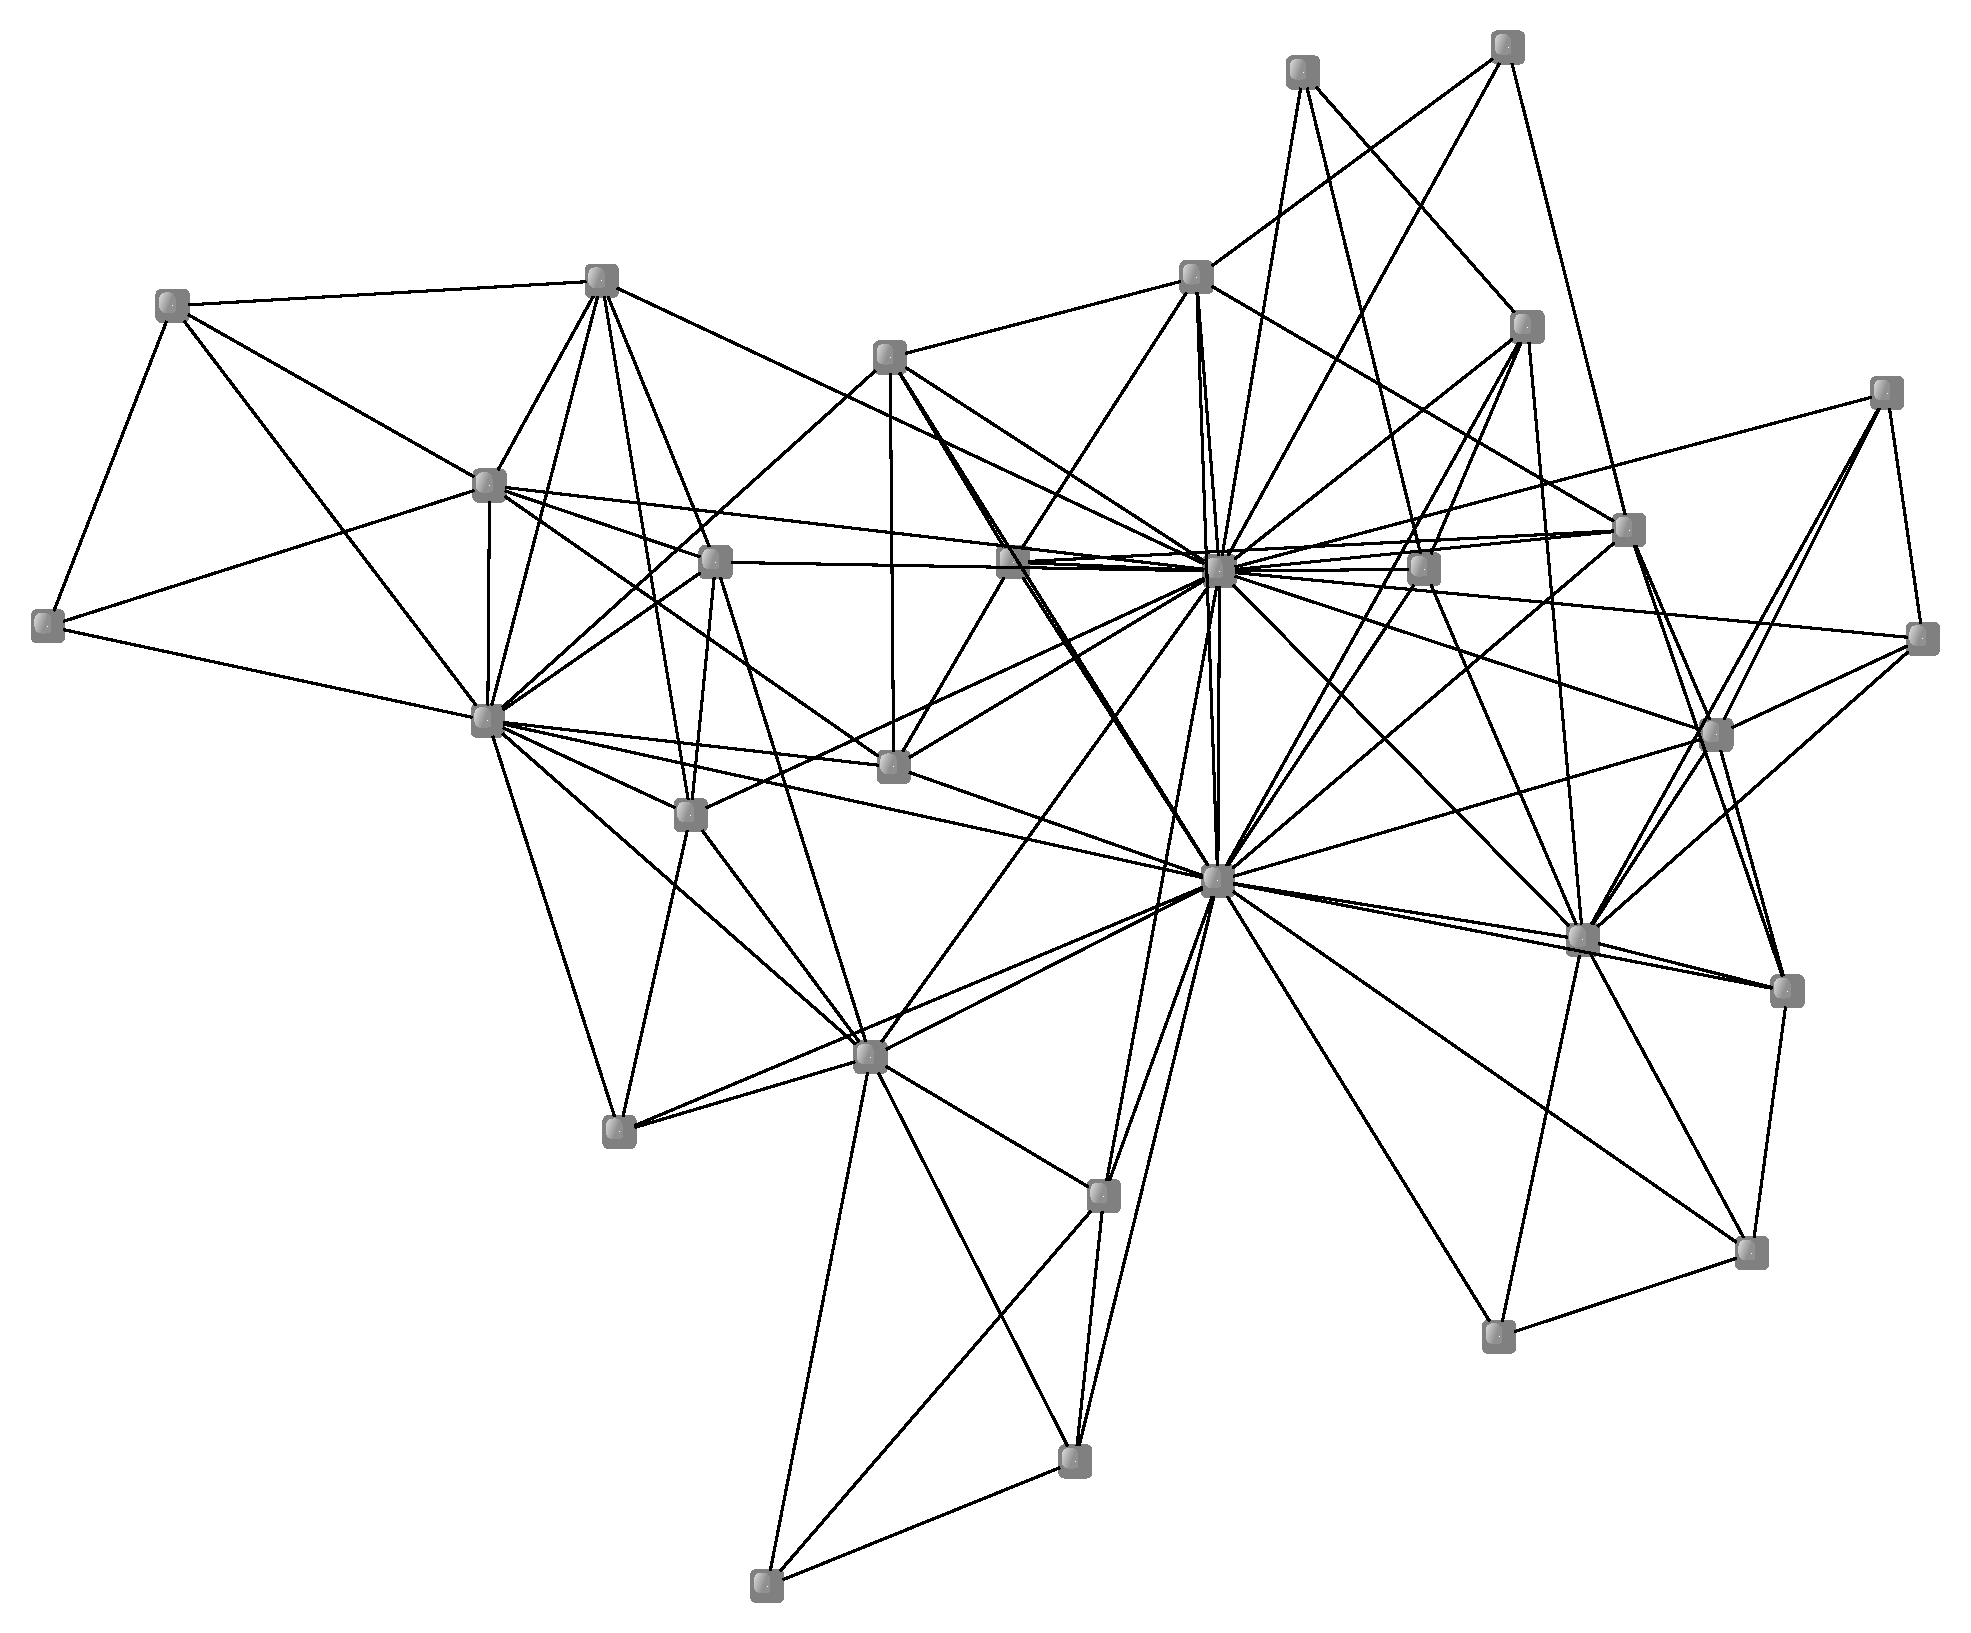
\includegraphics[width=0.4\textwidth]{graph5-yfiles}}

\subfloat[\label{fig:graph9-yfiles}{}]{
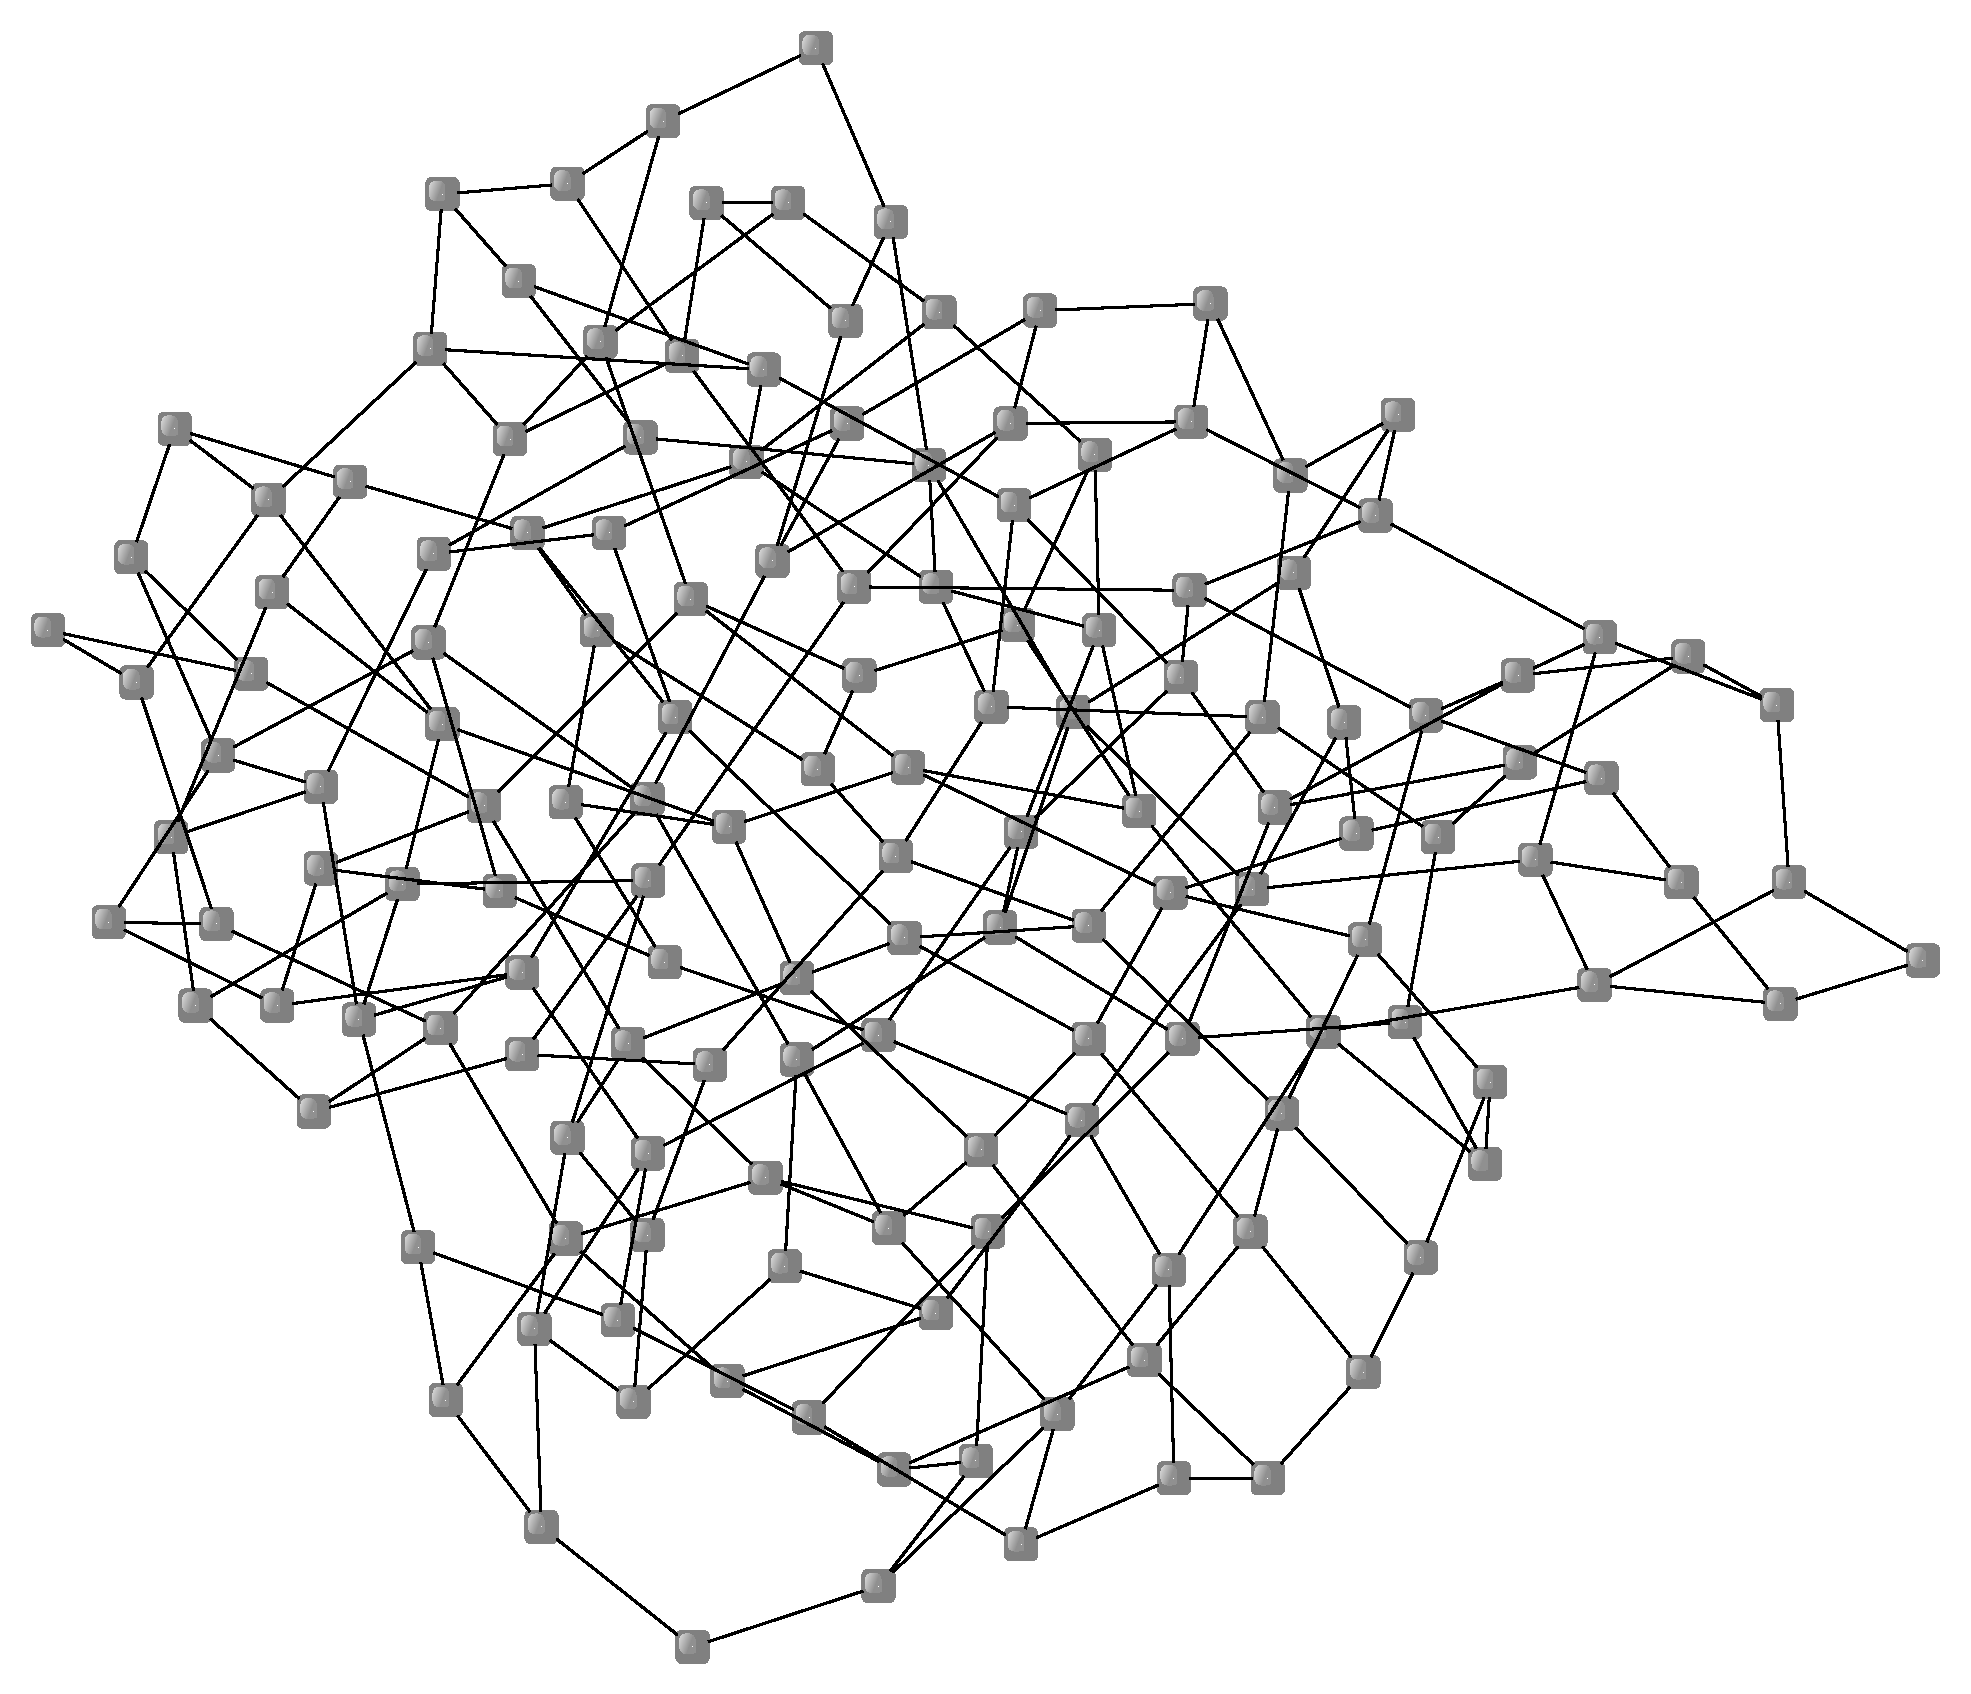
\includegraphics[width=0.37\textwidth]{graph9-yfiles}}
\caption{Illustration of 
(a)~the 5th, and of
(b)~the 9th graph of the Graph Drawing contest 2017.}
\label{fig:graph5And9-yfiles}
\end{figure}

% ==================================================================
\section{Conclusions}
\label{sec:conclusions}
% ==================================================================

%
In this paper, we introduced a new heuristic aiming to produce drawings of high crossing resolution, for which we also presented variants that take into account other common aesthetic criteria in Graph Drawing. Our experimental evaluation indicates that the new heuristic is competitive to the state of the art force-directed algorithms, even when restricted to a given maximum aspect ratio. 

It also worth noting that while working on this project, we made some useful observations and obtained some interesting insights. In particular, there is a recent observation (also supported by experiments) that drawings, in which the crossing angles are large, are easy to read and understand. We observed that drawings that are optimized only in terms of the crossing angles might be arbitrarily bad and may have several undesired properties. In particular, in these drawings it was very common to have adjacent edges to run almost in parallel and vertices to be very close to each other (see, e.g., Fig.~\ref{fig:graph5-argyriou-cr}). Hence, their angular resolution and aspect ratio were often poor. The additional restrictions that we imposed regarding the angular resolution and the aspect ratio helped in significantly improving the readability of the produced drawings, without loosing too much of their quality in terms of the crossing resolution.

We conclude by noting that our motivation to work with this problem was our participation to the Graph Drawing contest 2017, where we performed miserably using a force-directed algorithm. As our evaluation shows, the performance of such algorithms is good, only when several aesthetic criteria are taken into account. 

The framework that we developed seems to be quite adaptable to optimize or to take into account also other desired aesthetic properties of a drawing. Thus, as a future direction, we plan to further extend and evaluate our technique, e.g., by using a multi-criteria objective function (i.e., that is not limited to the crossing angles) that takes into account more aesthetic criteria. 

\paragraph{Acknowledgments.} The authors would also like to thank Simon Wegendt and Jessica Wolz for implementing the first version of our prototype.

\bibliographystyle{compj}
\bibliography{references}

\clearpage

\begin{figure*}[h!]
	\centering
	\subfloat[\label{fig:graph5-ourBest-cr}{Crossing Resolution}]{
	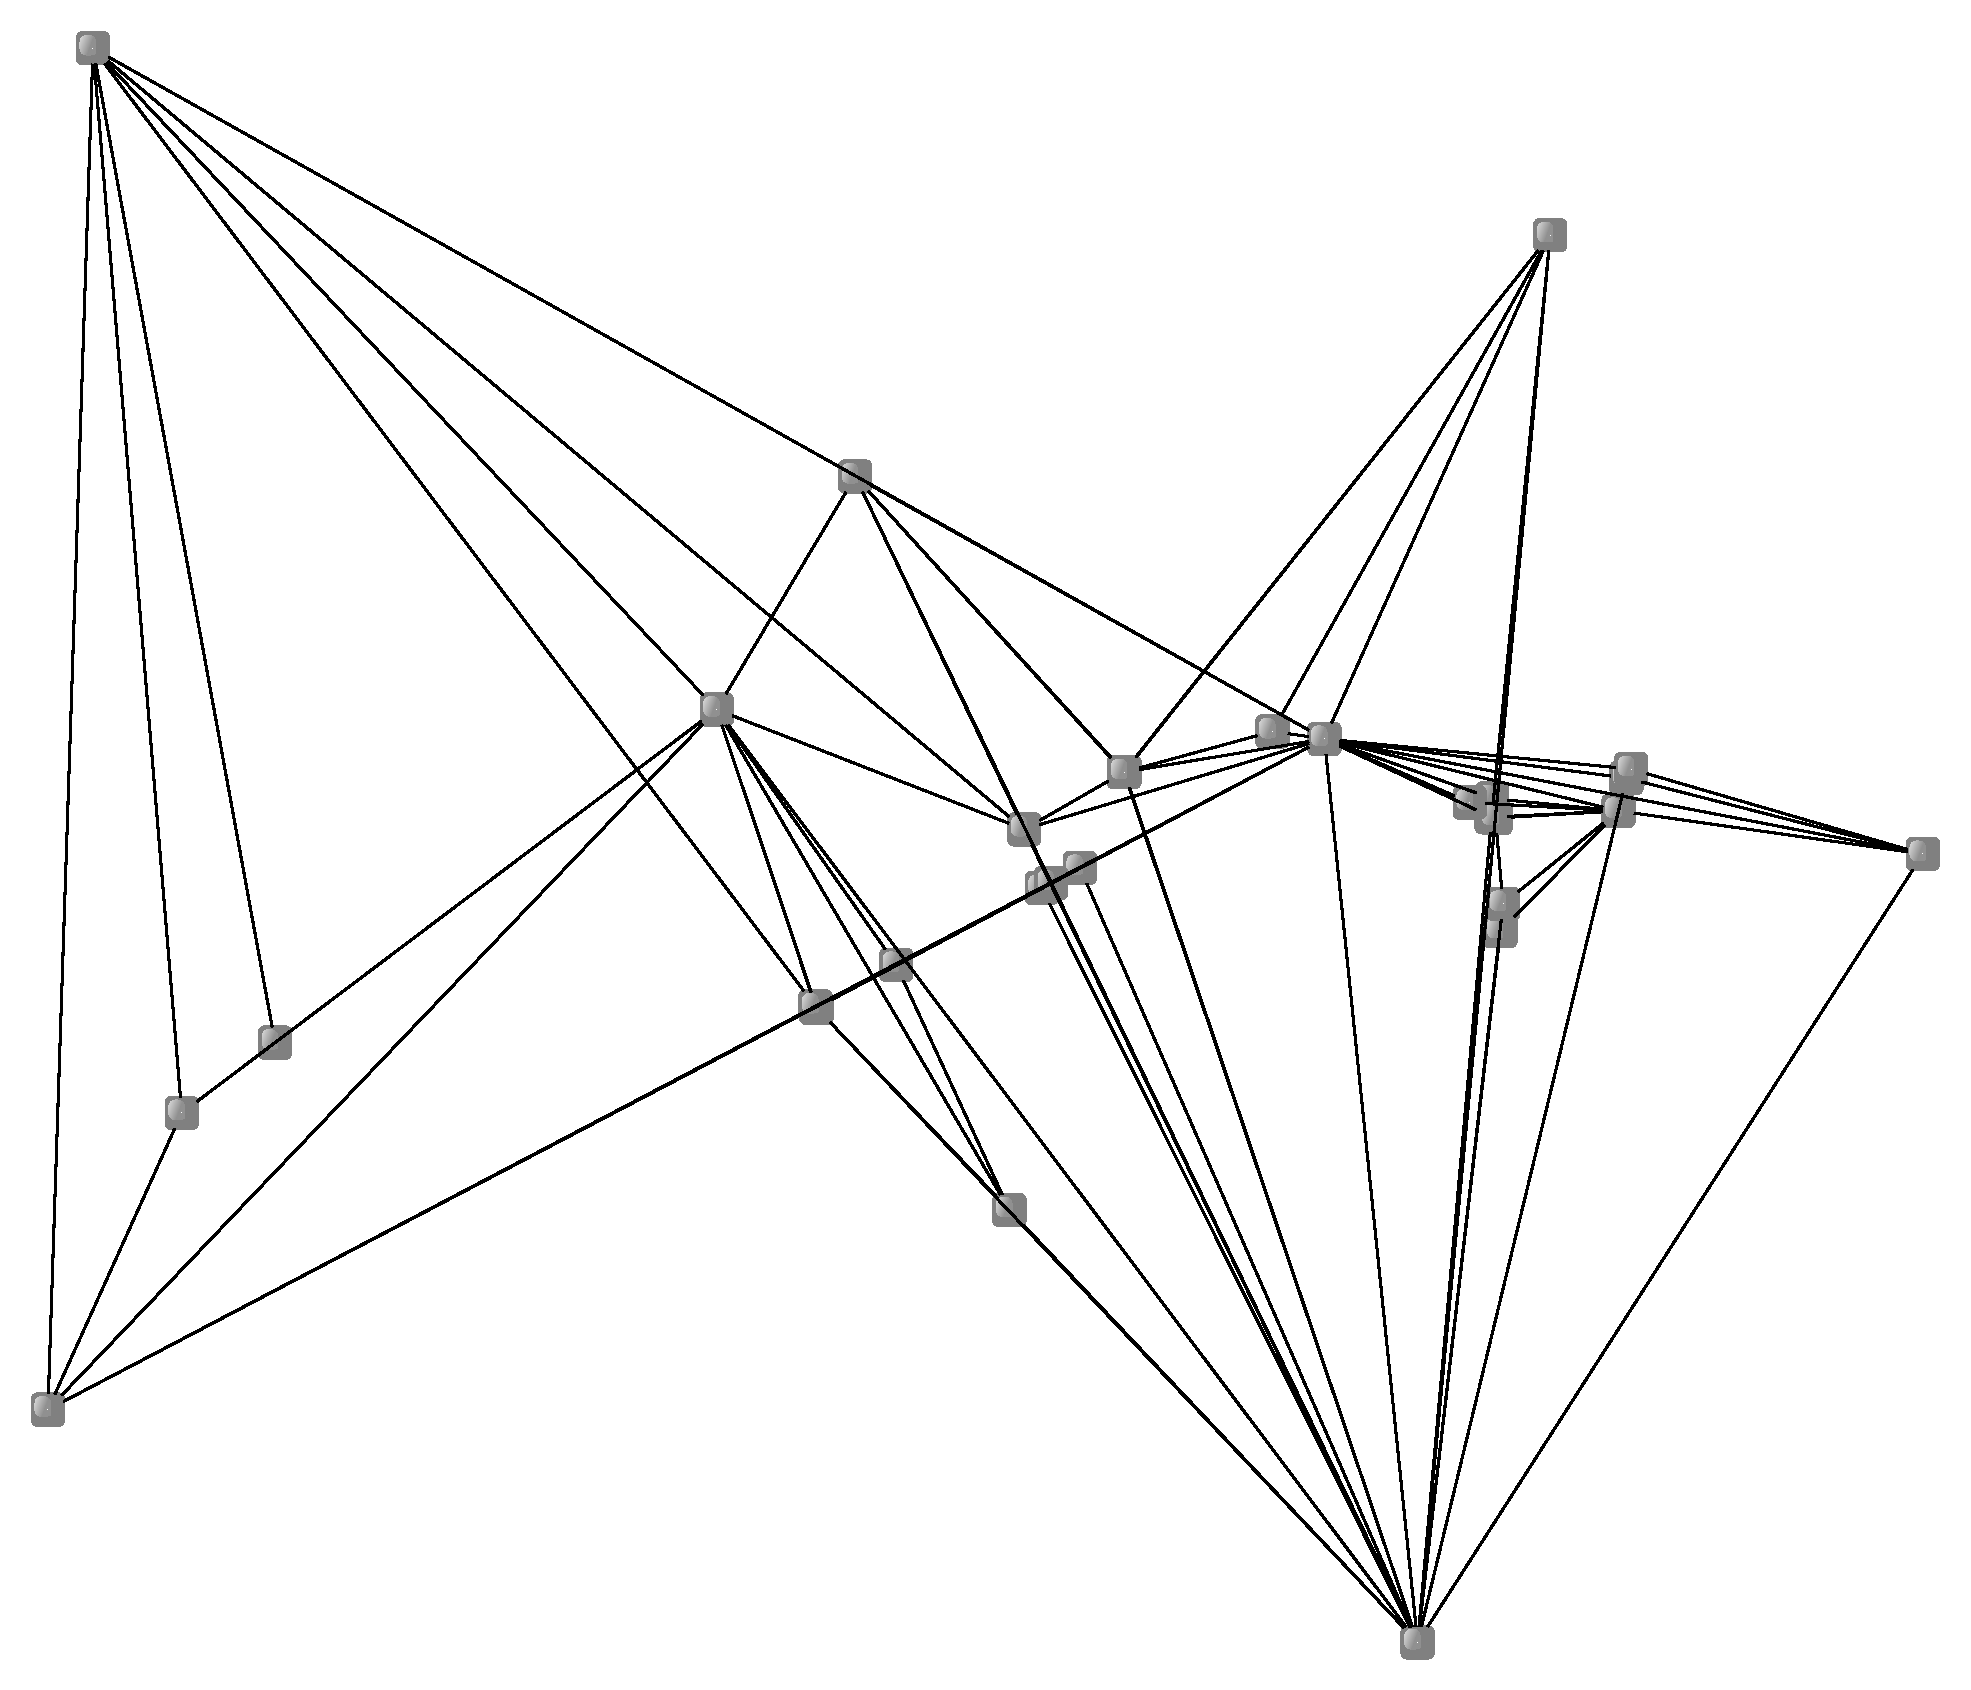
\includegraphics[width=0.27\textwidth]{graph5-ourBest-crossing}}
	\hfill
	\subfloat[\label{fig:graph5-ourBest-ar}{Angular Resolution}]{
	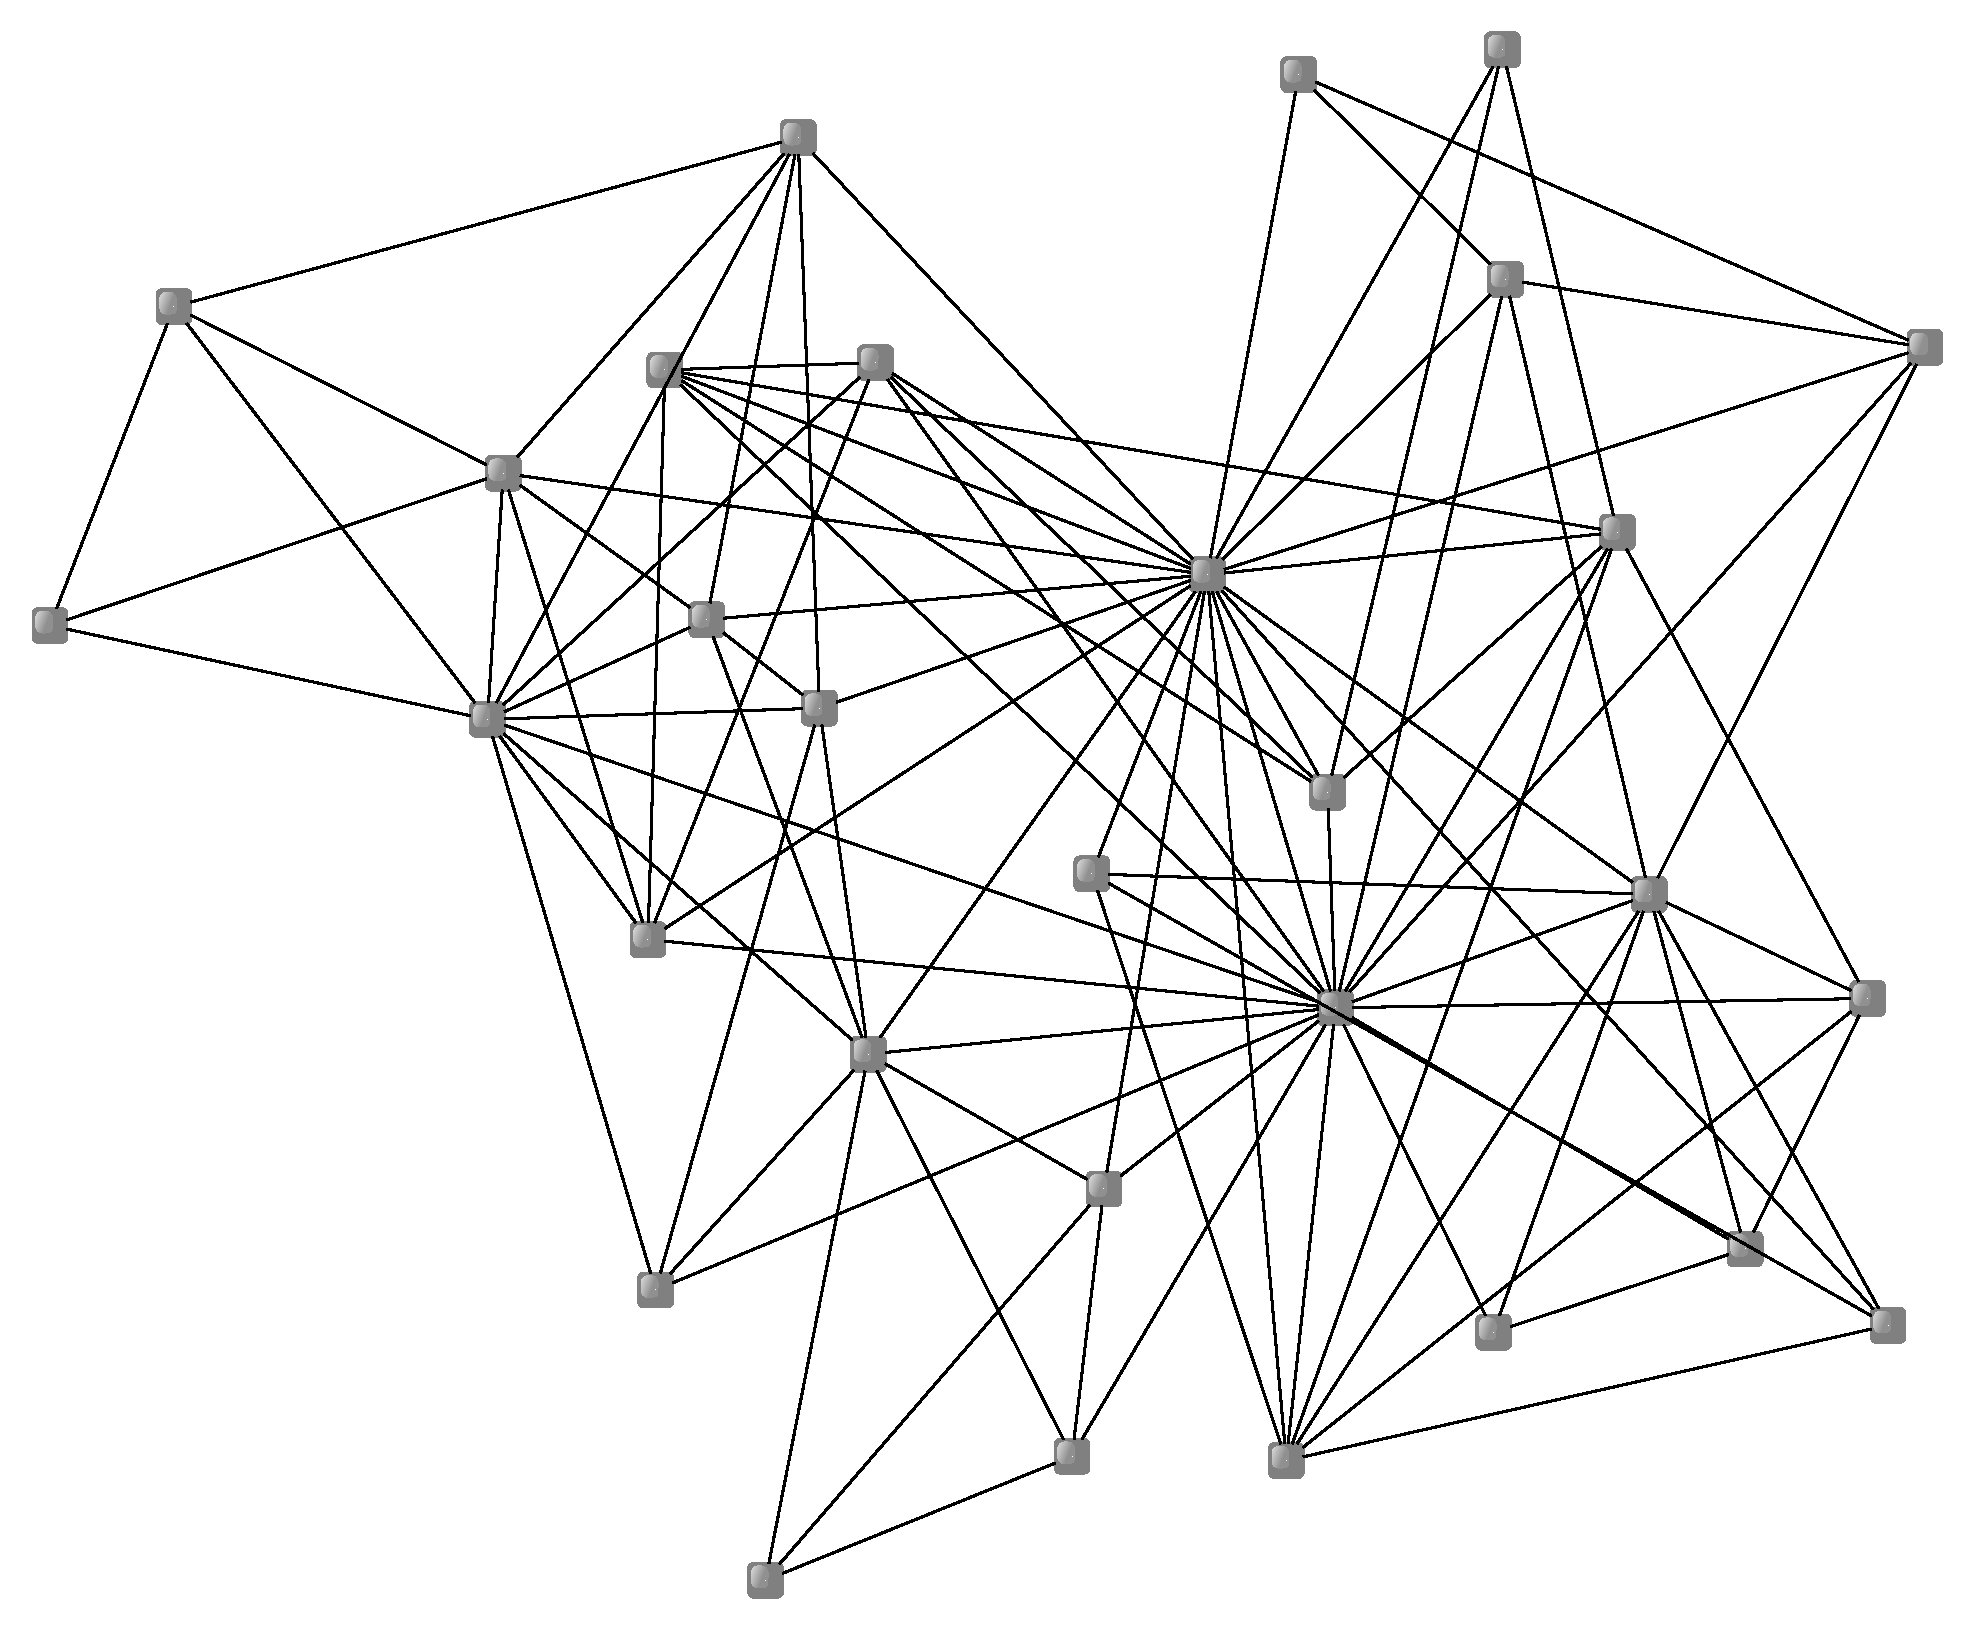
\includegraphics[width=0.27\textwidth]{graph5-ourBest-angular}}
	\hfill
	\subfloat[\label{fig:graph5-ourBest-tr}{Total Resolution}]{
	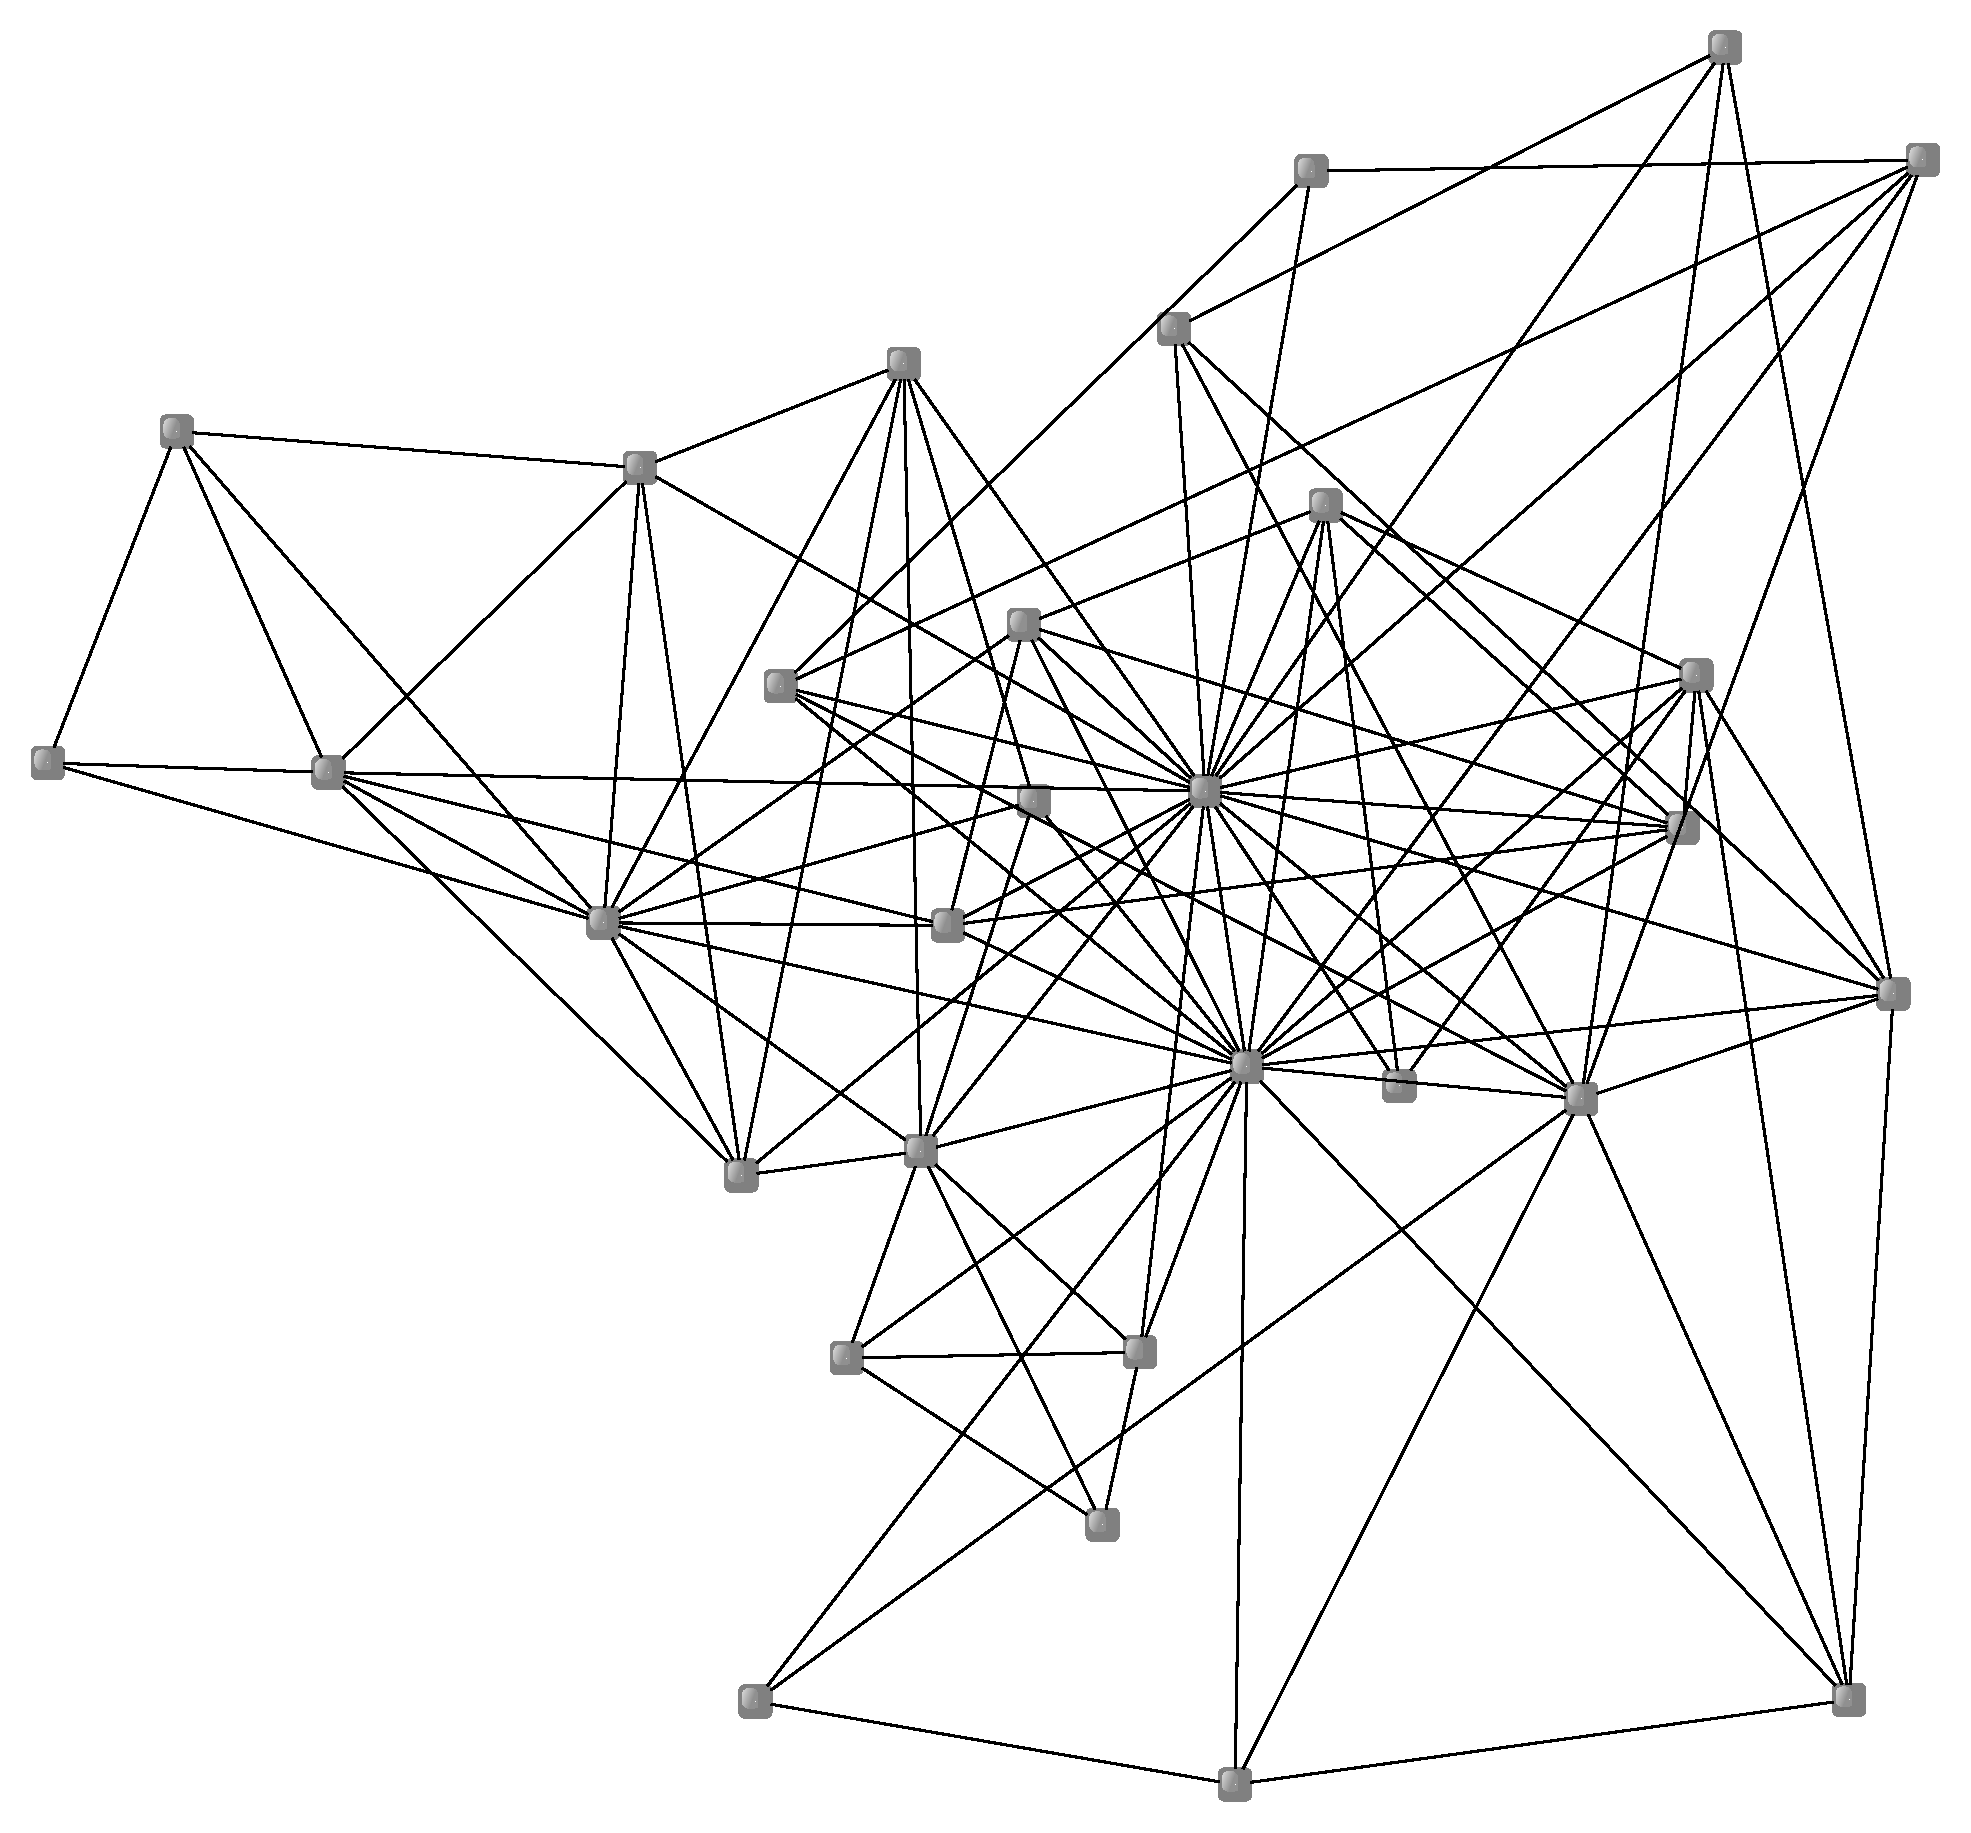
\includegraphics[width=0.27\textwidth]{graph5-ourBest-total}}
	\hfill
	\subfloat[\label{fig:graph5-ourRestricted-cr}{Crossing Resolution}]{
	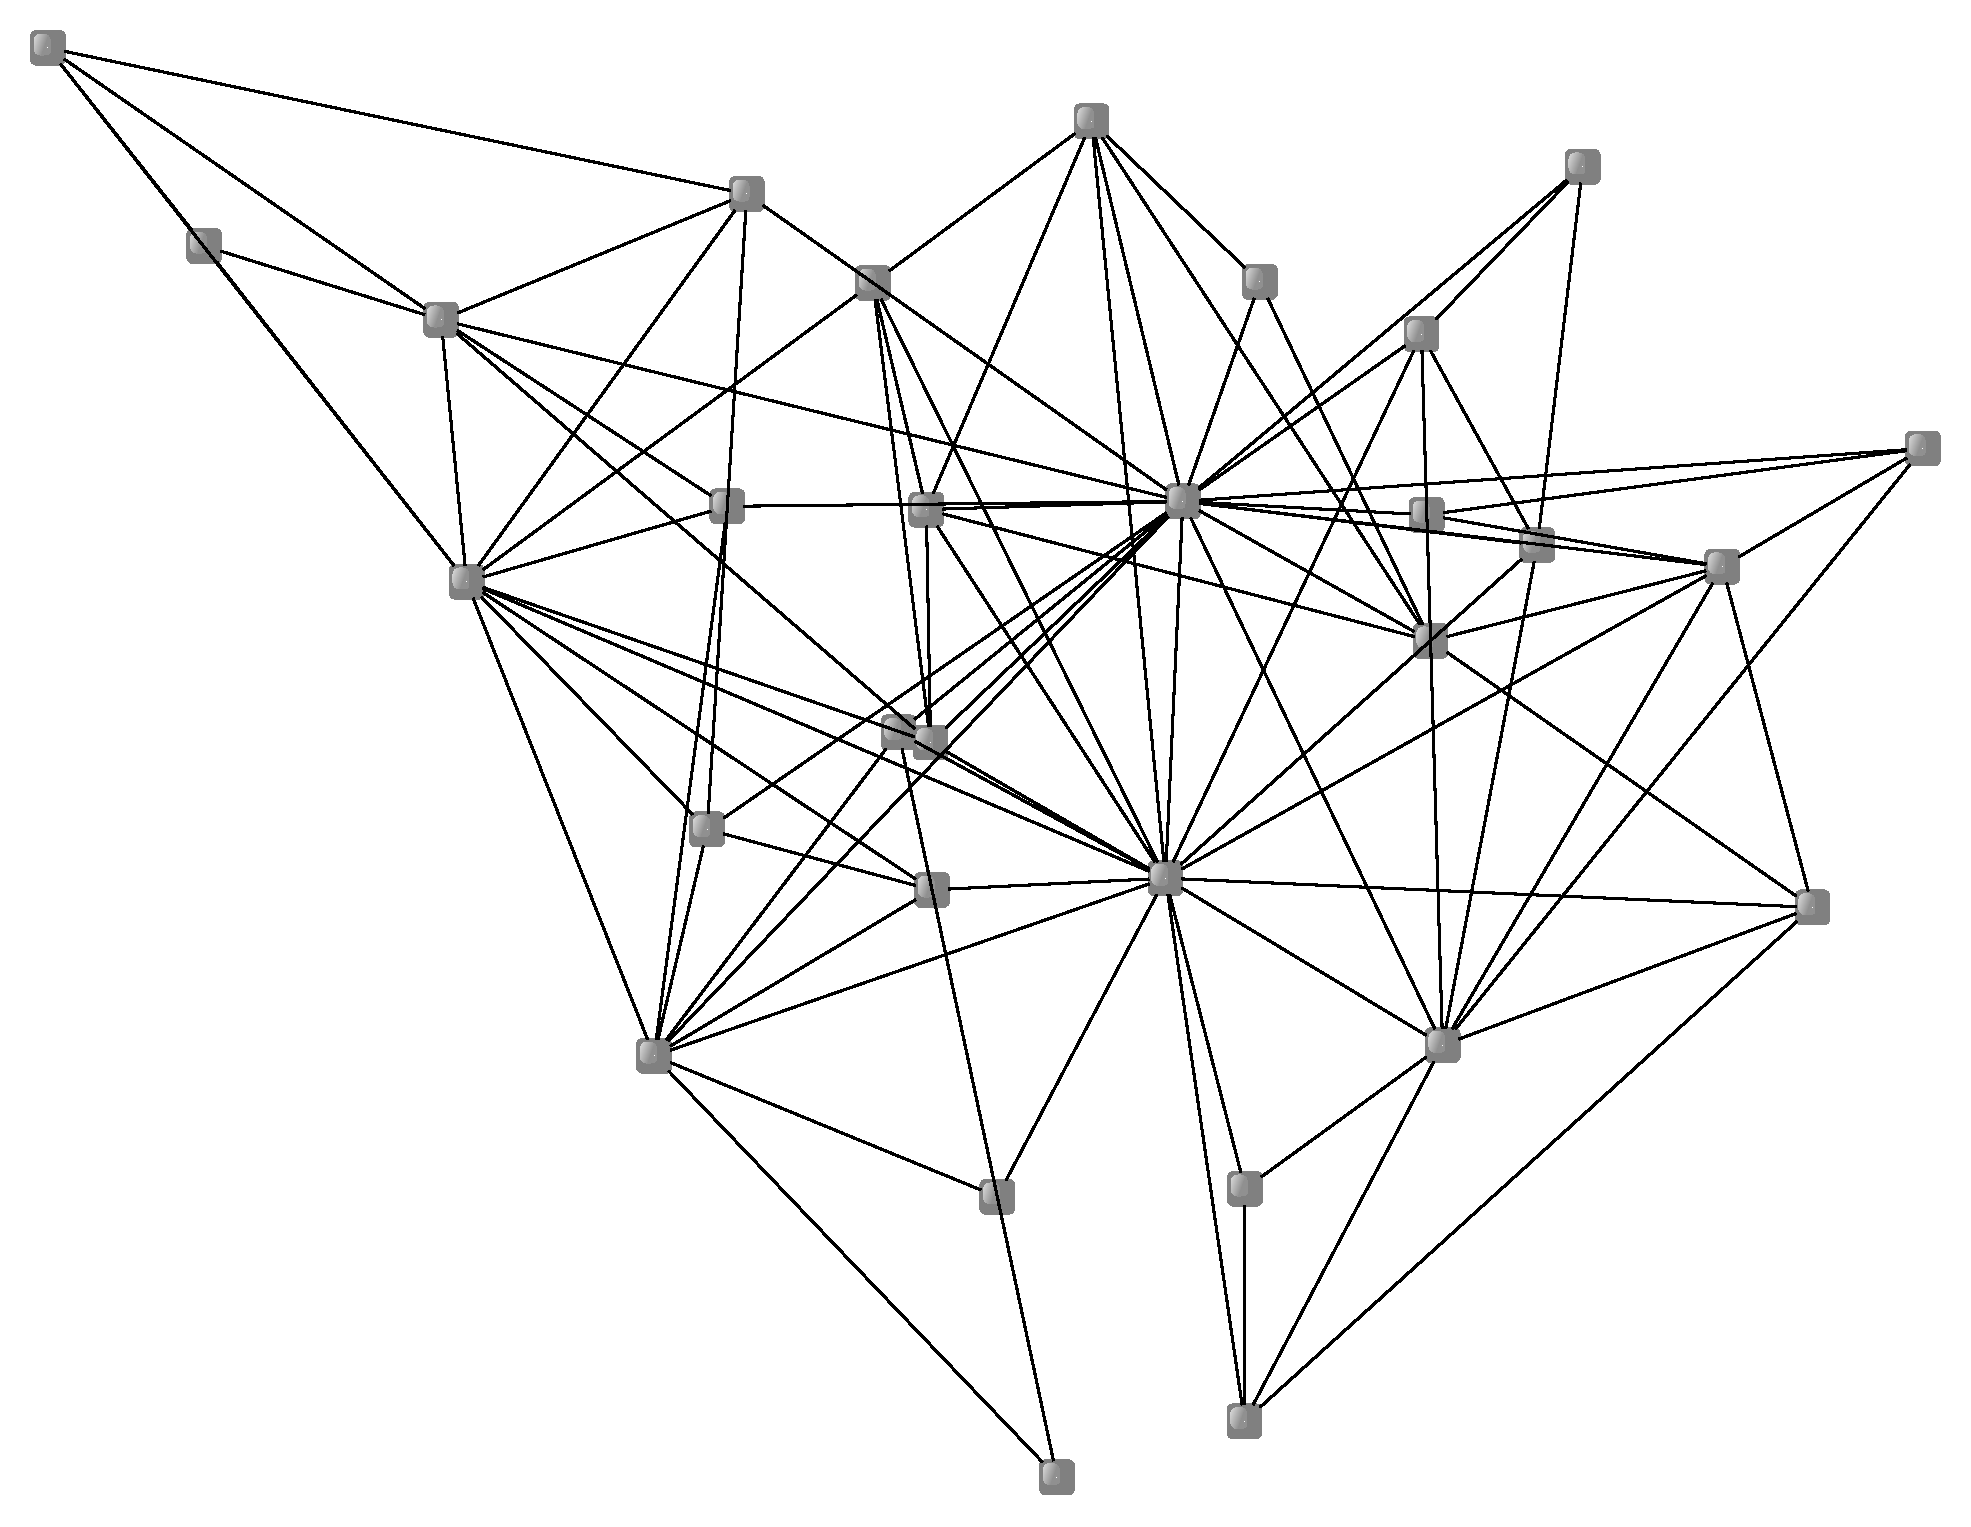
\includegraphics[width=0.27\textwidth]{graph5-ourRestricted-crossing}}
	\hfill
	\subfloat[\label{fig:graph5-ourRestricted-ar}{Angular Resolution}]{
	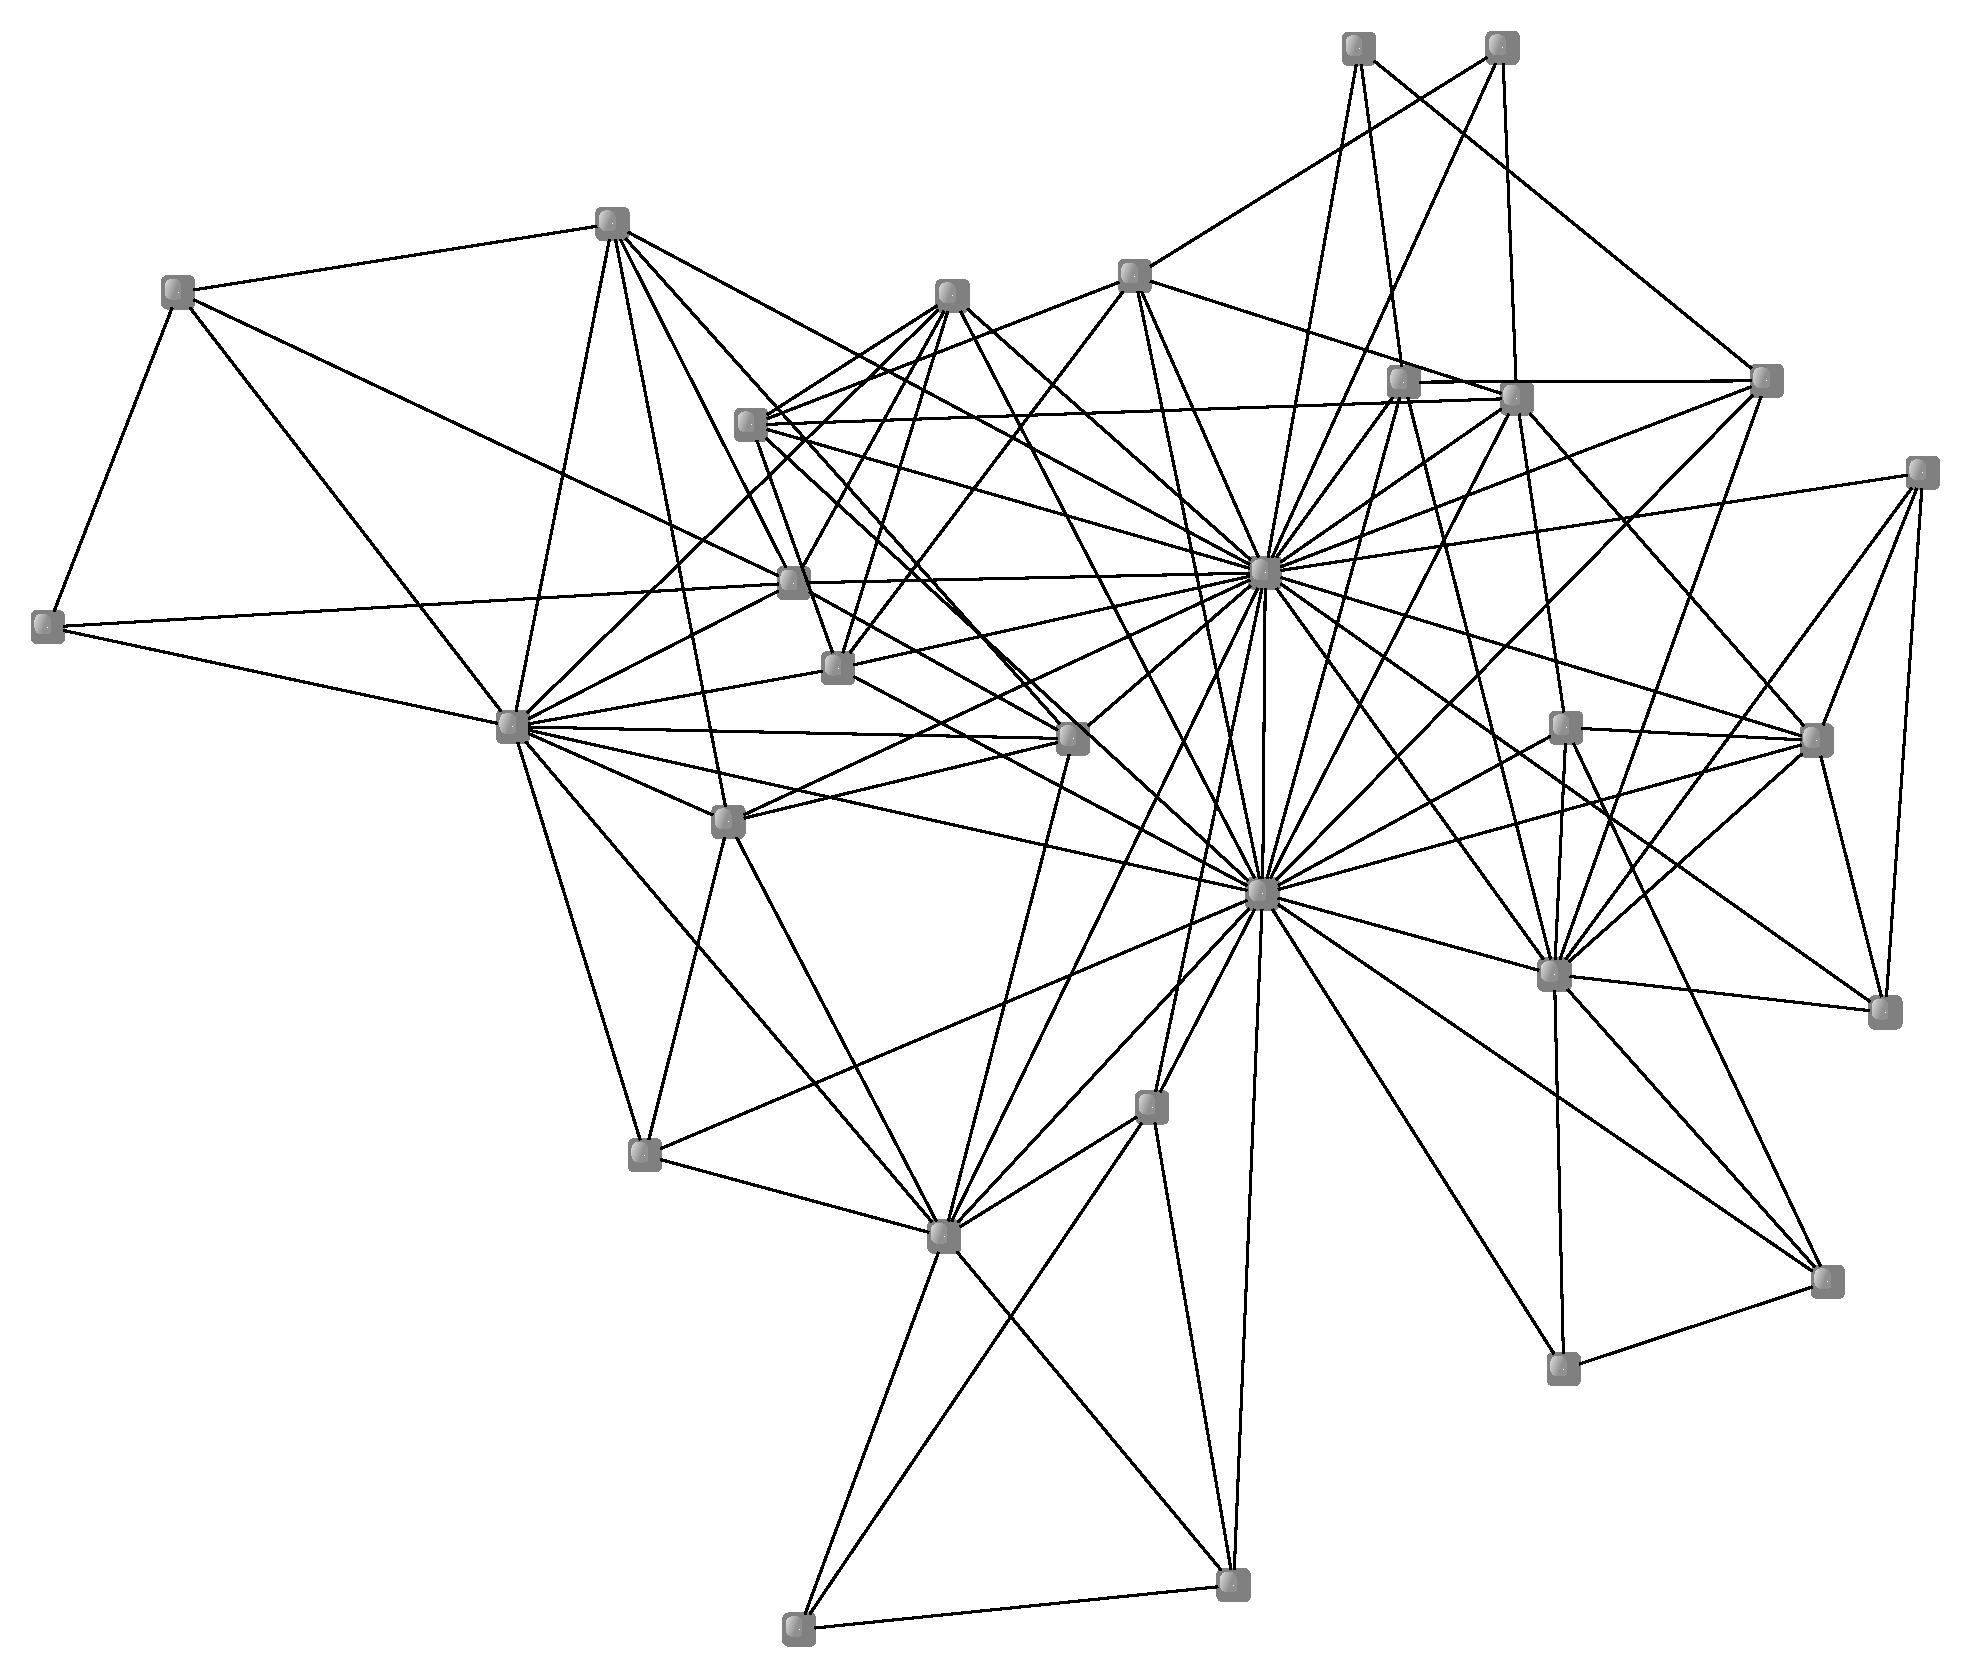
\includegraphics[width=0.27\textwidth]{graph5-ourRestricted-angular}}
	\hfill
	\subfloat[\label{fig:graph5-ourRestricted-tr}{Total Resolution}]{
	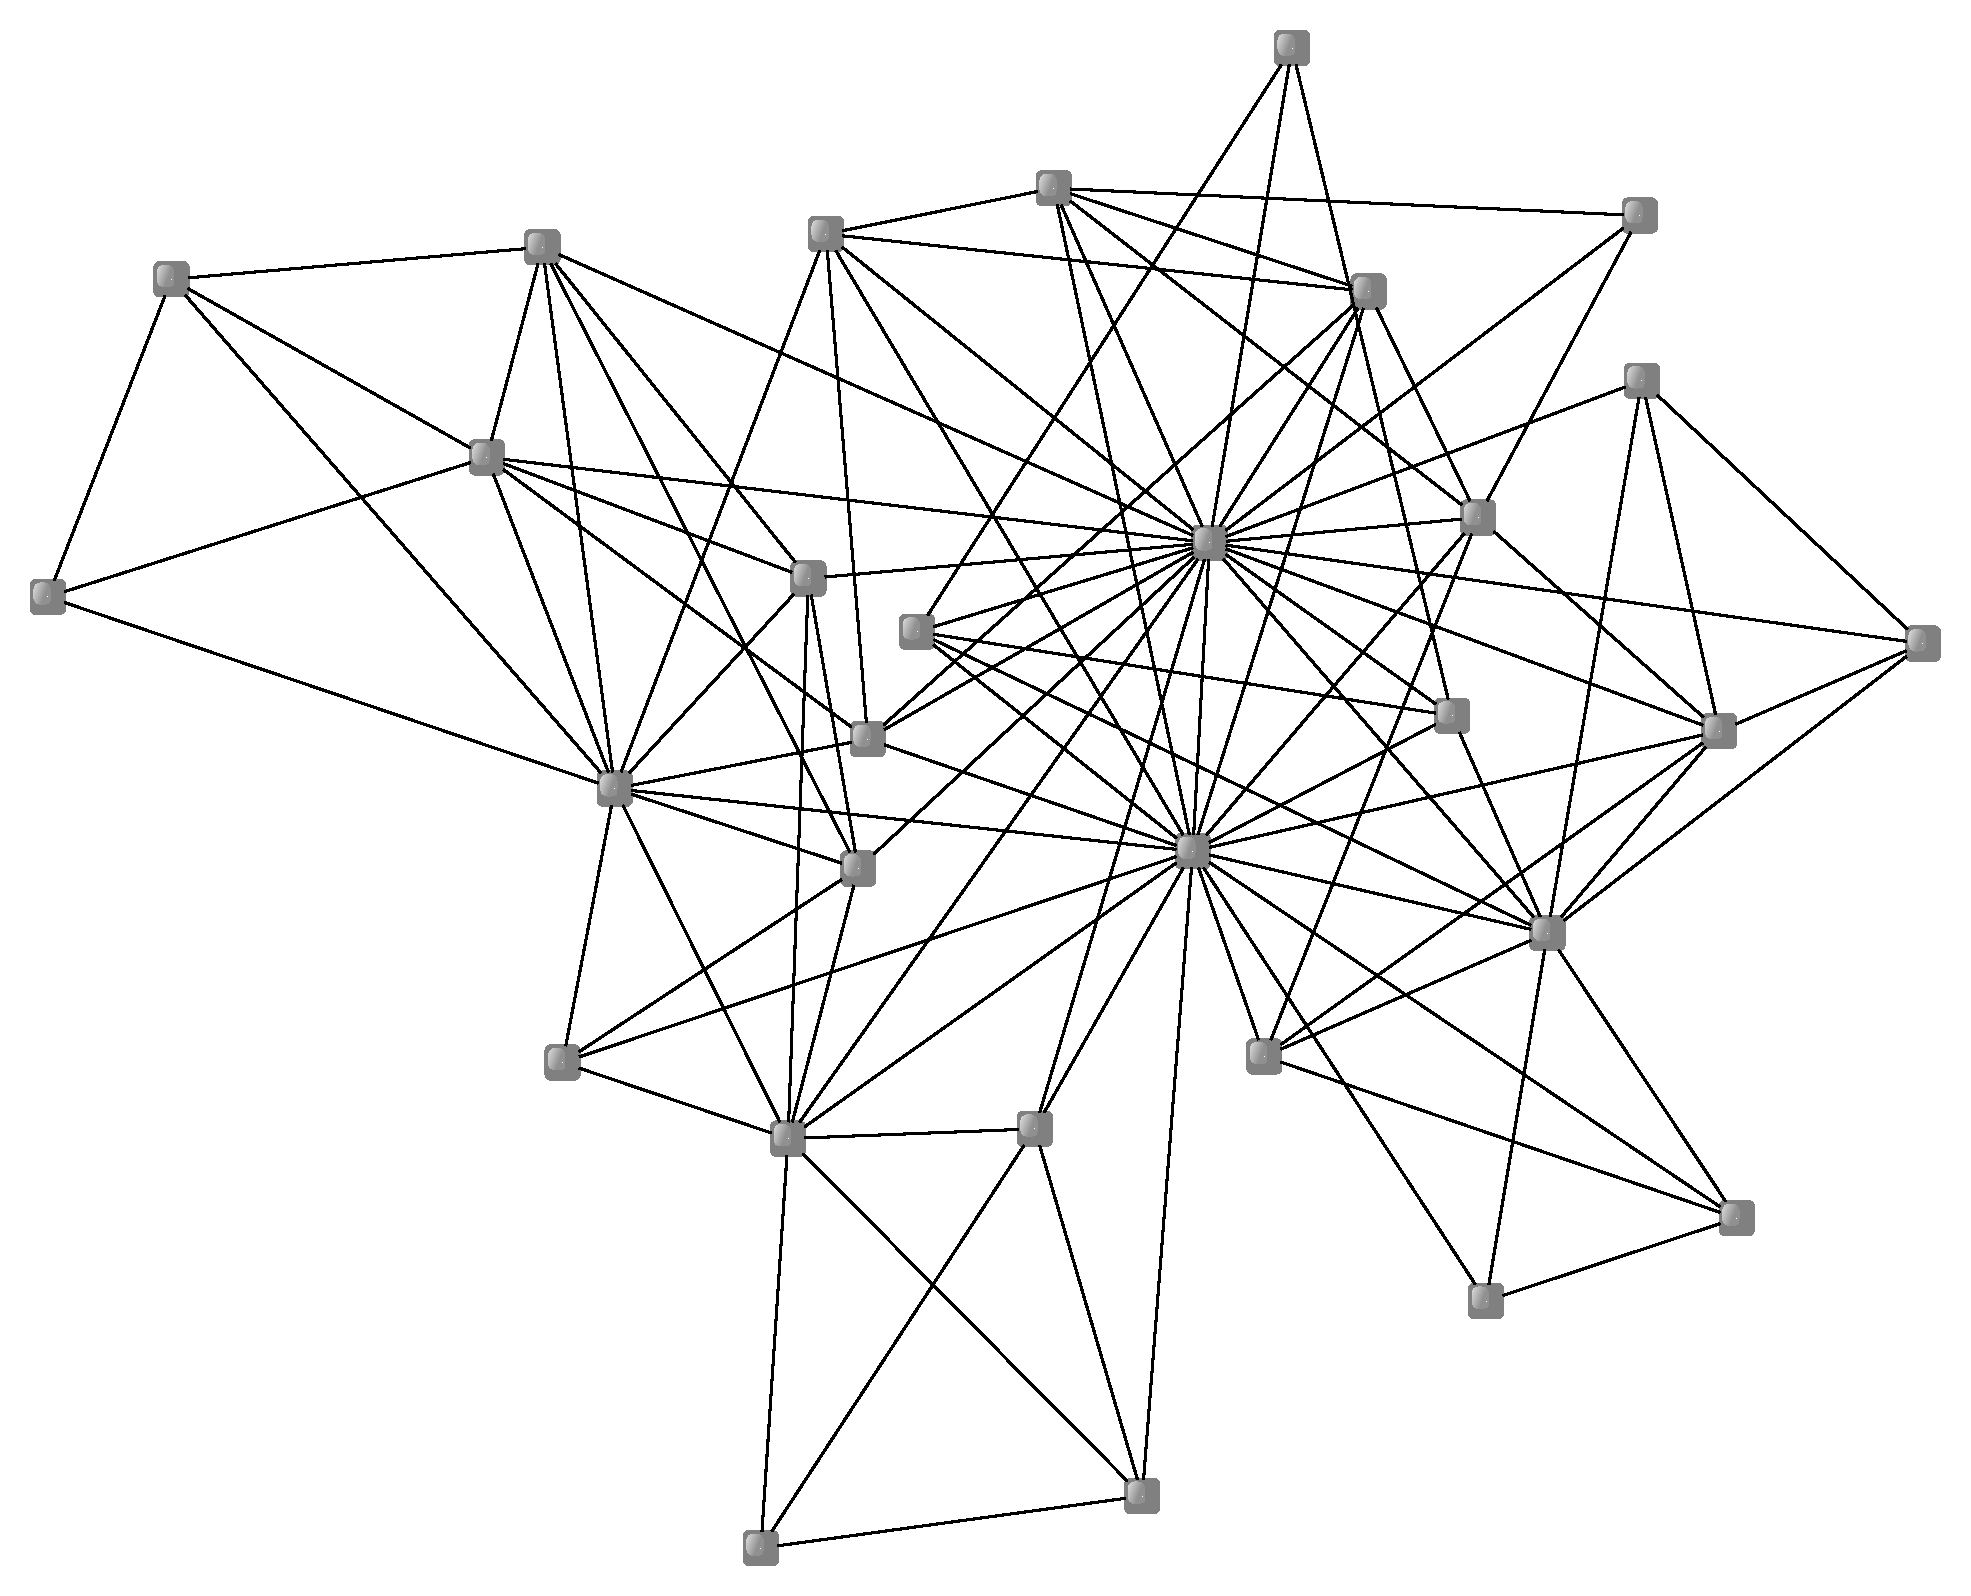
\includegraphics[width=0.27\textwidth]{graph5-ourRestricted-total}}
	\hfill
	\subfloat[\label{fig:graph5-argyriou-cr}{Crossing Resolution}]{
	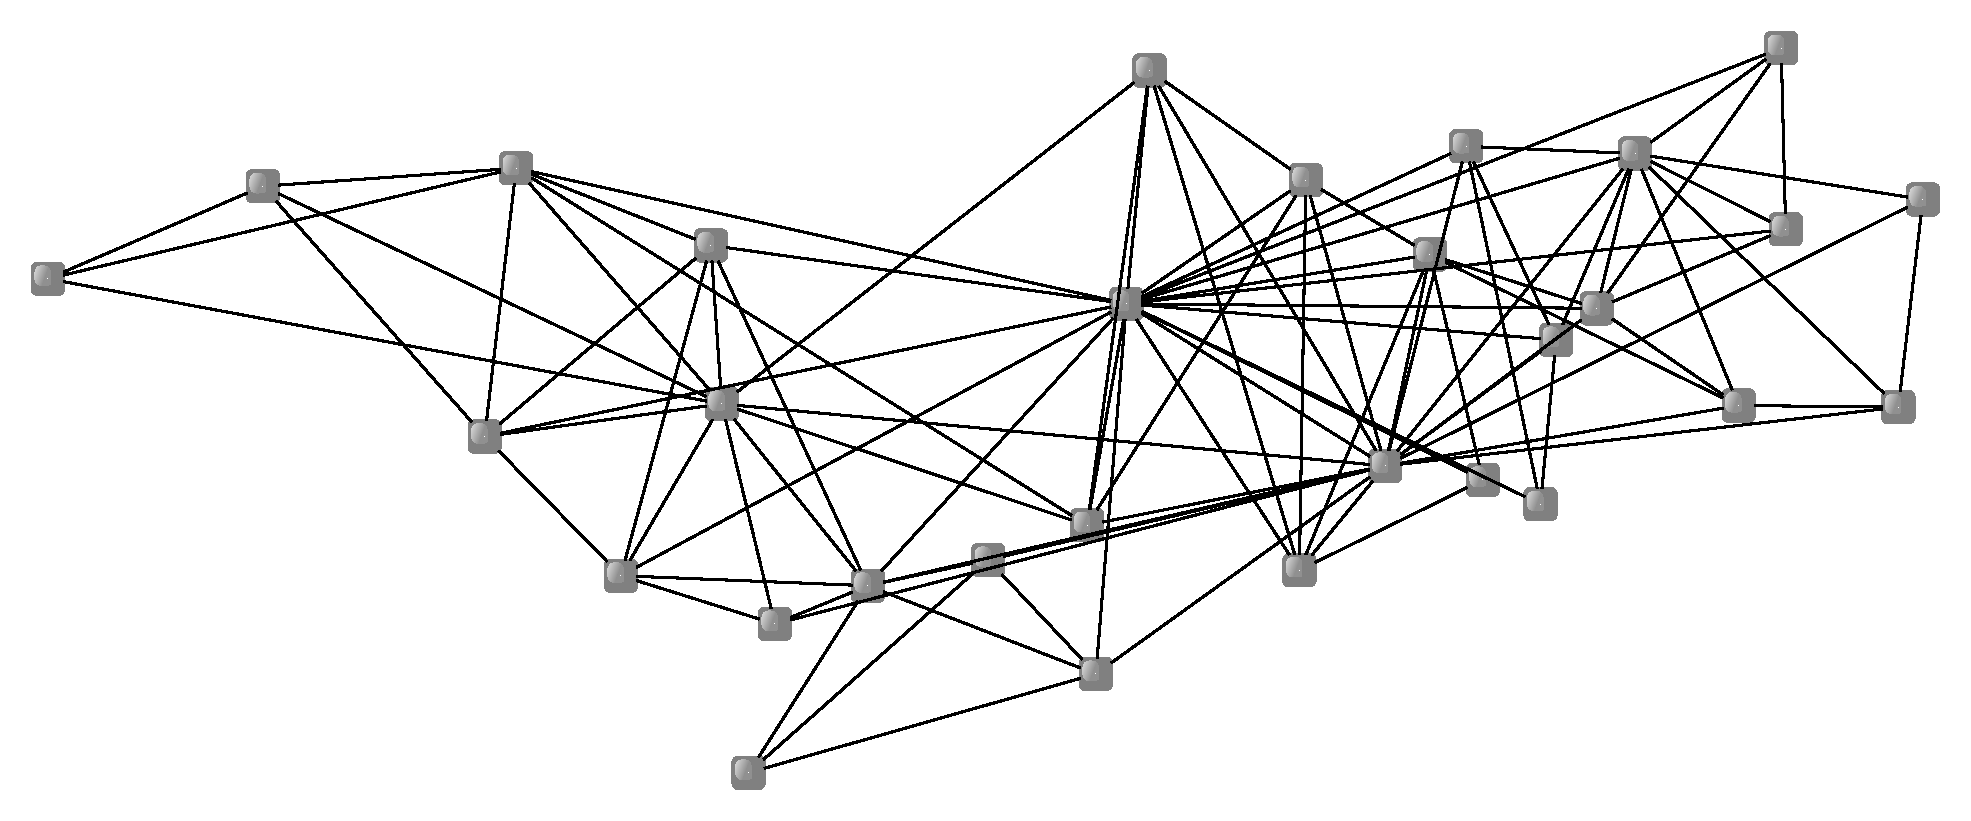
\includegraphics[width=0.27\textwidth]{graph5-argyriou-crossing}}
	\hfill
	\subfloat[\label{fig:graph5-argyriou-ar}{Angular Resolution}]{
	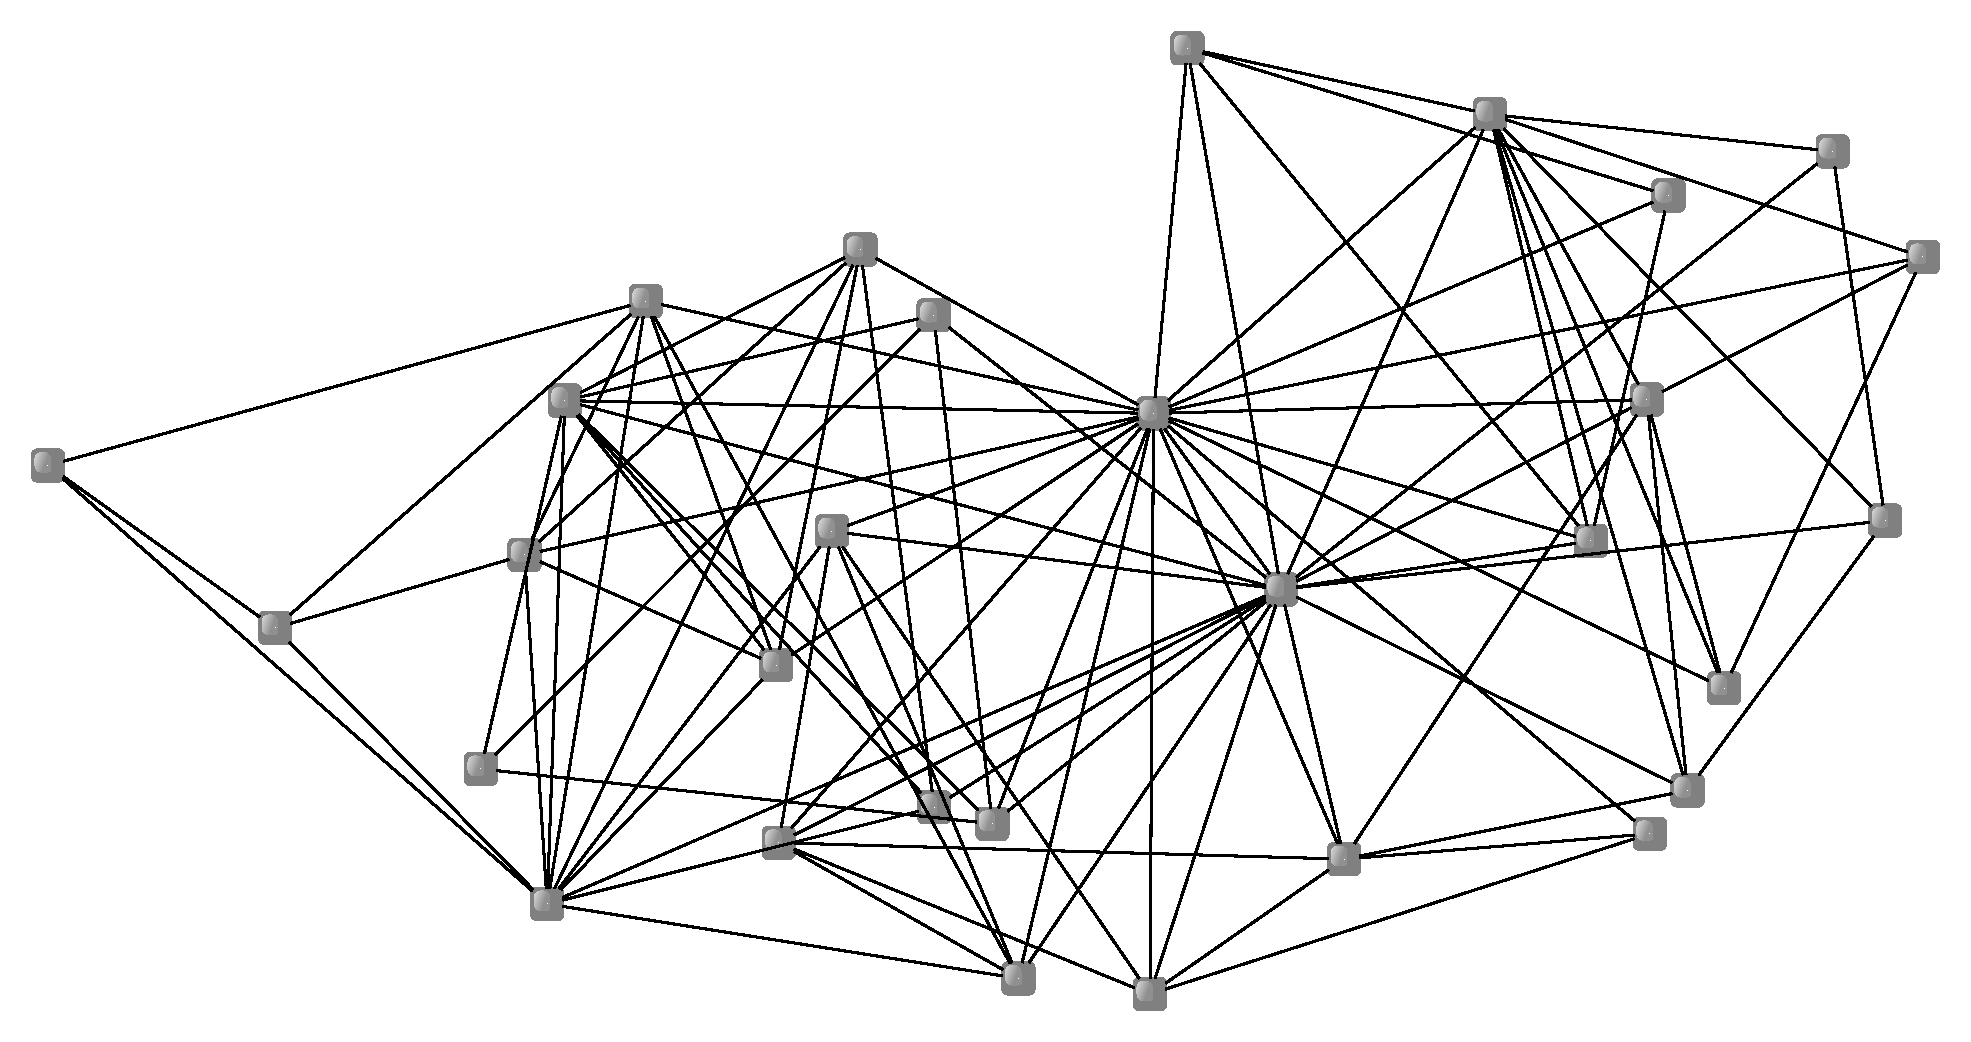
\includegraphics[width=0.27\textwidth]{graph5-argyriou-angular}}
	\hfill
	\subfloat[\label{fig:graph5-argyriou-tr}{Total Resolution}]{
	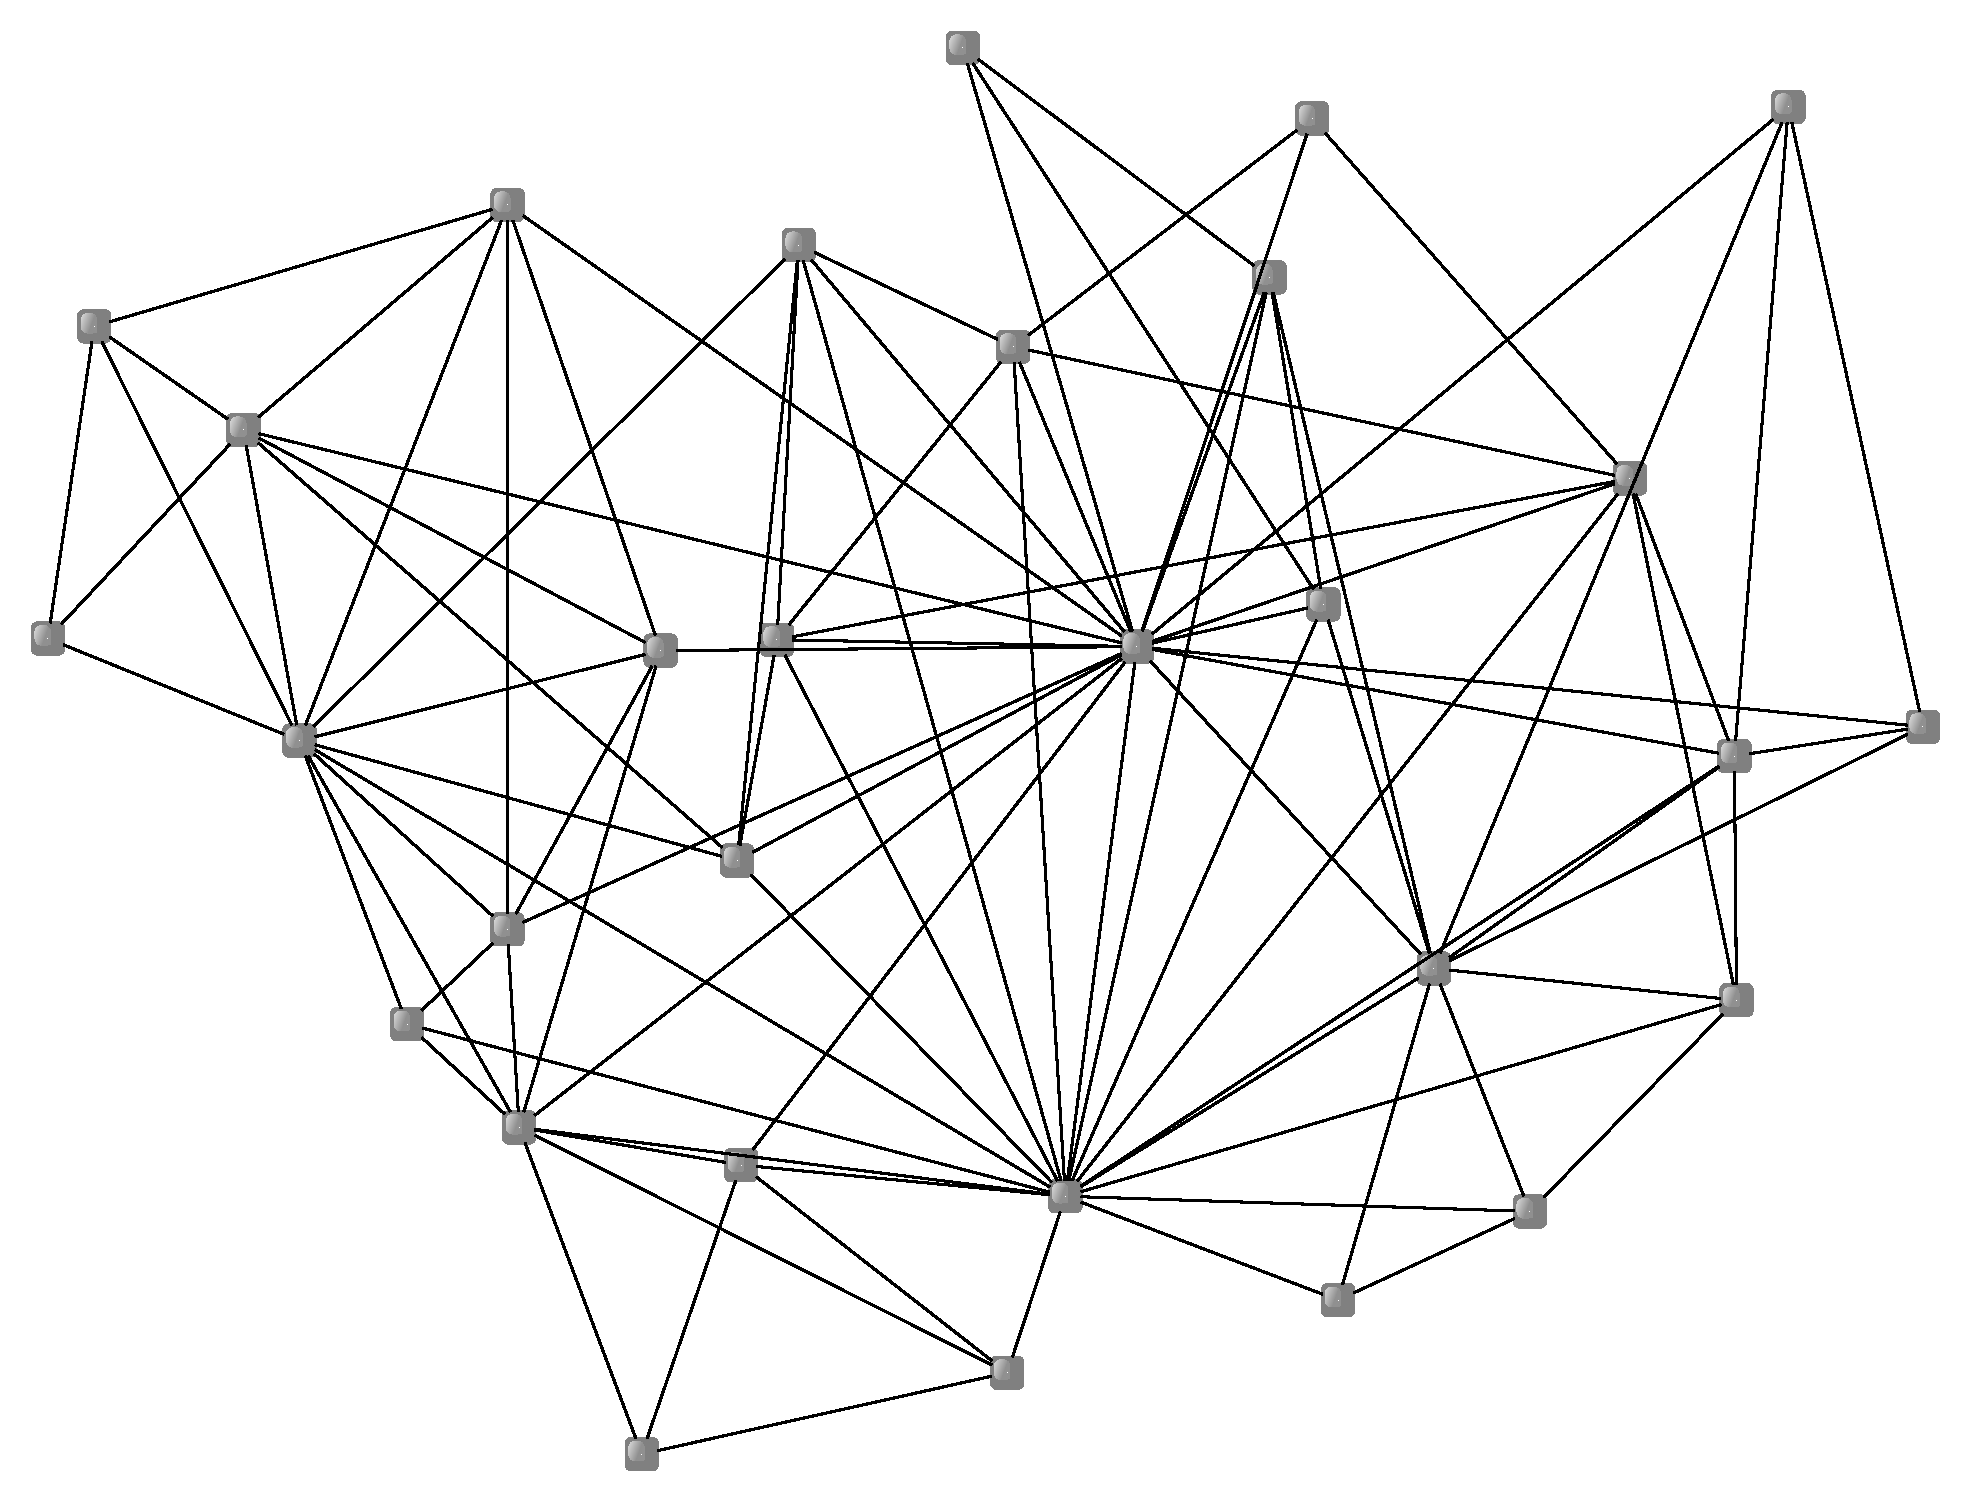
\includegraphics[width=0.27\textwidth]{graph5-argyriou-total}}
	\hfill
	\subfloat[\label{fig:graph5-huang-cr}{Crossing Resolution}]{
	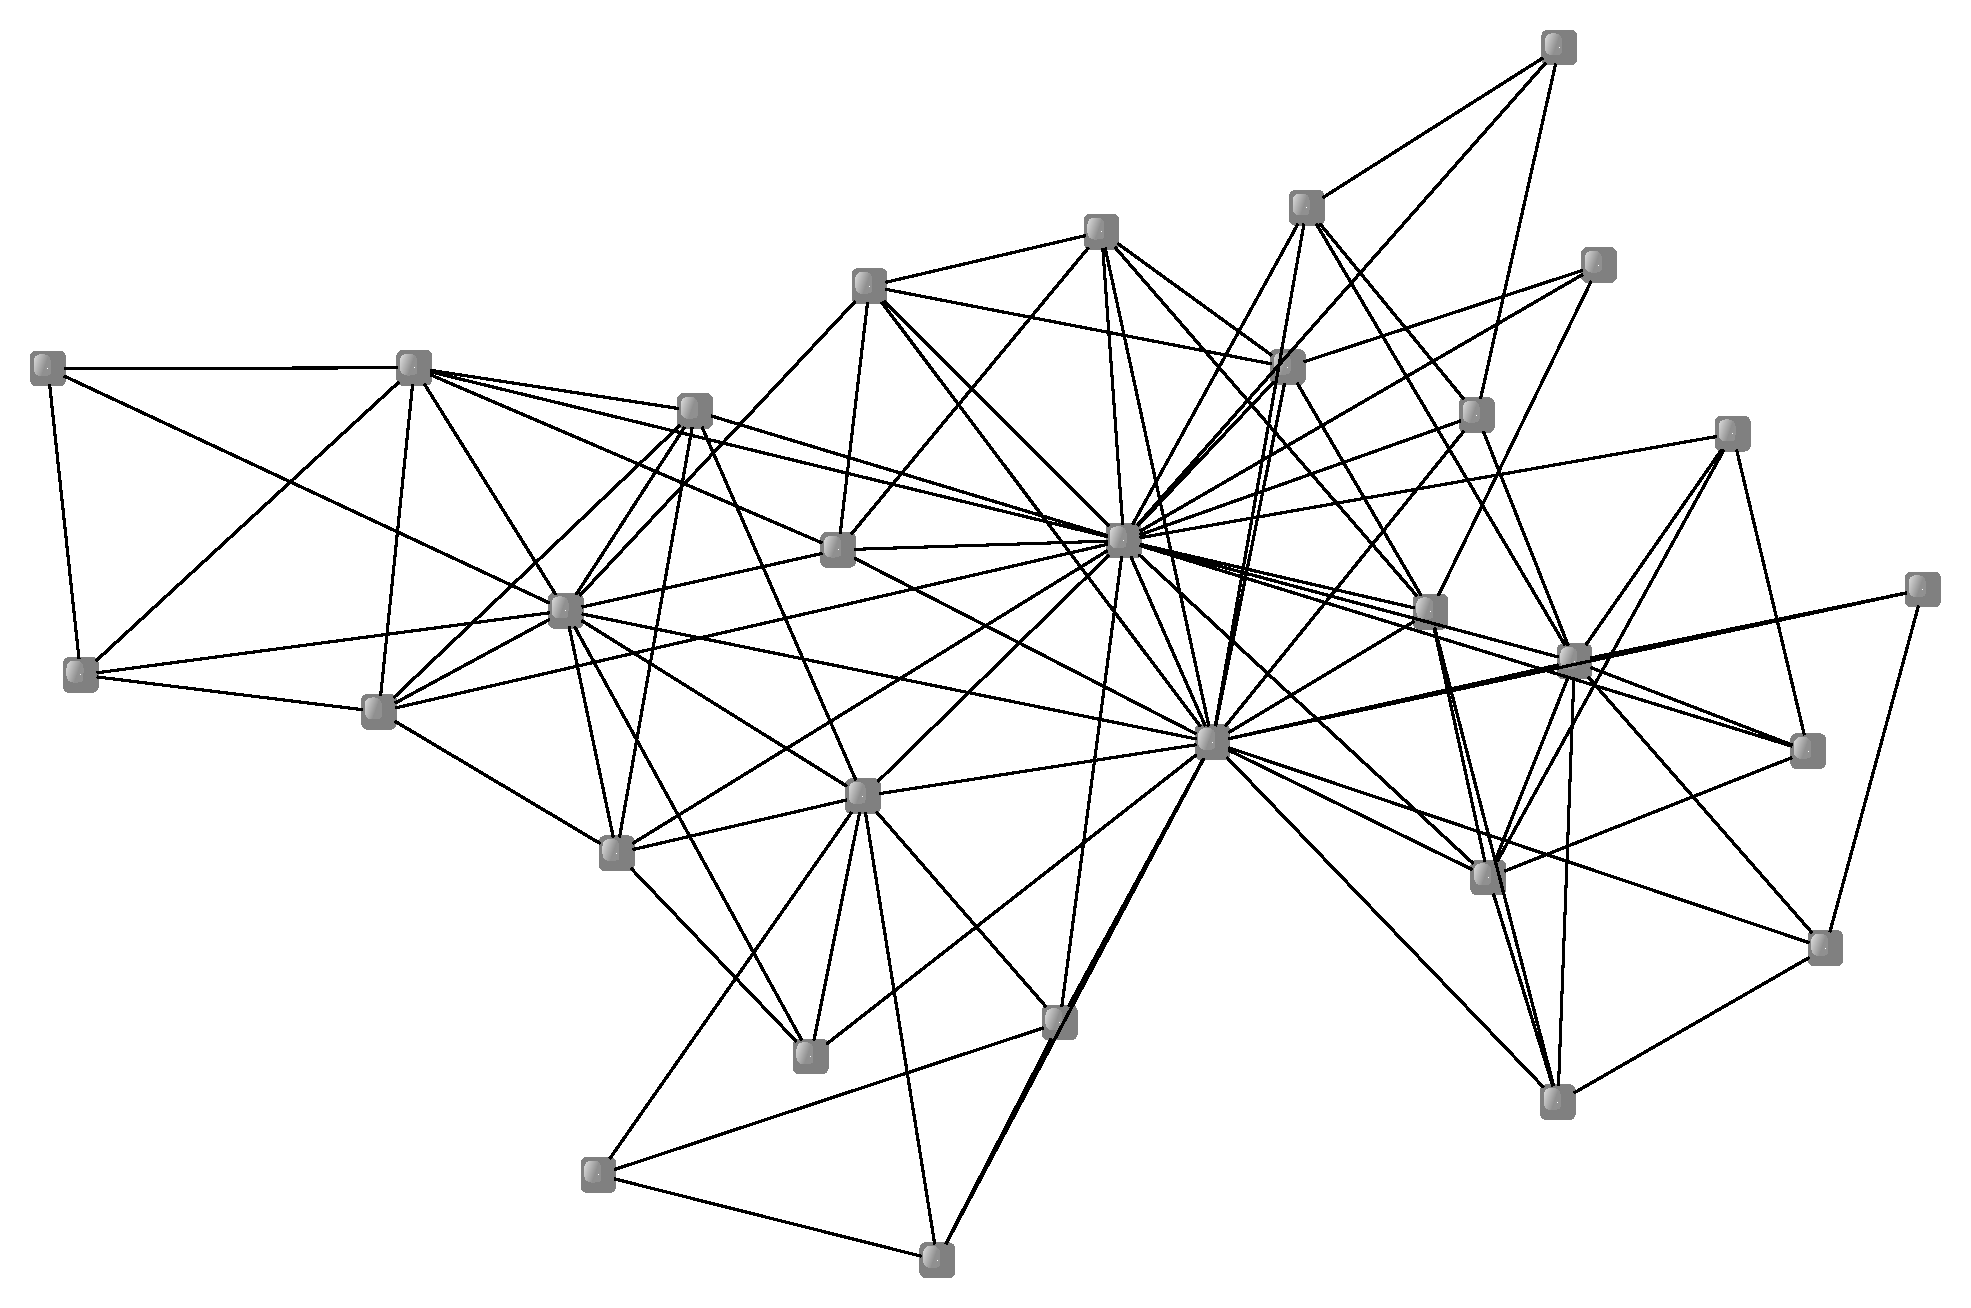
\includegraphics[width=0.27\textwidth]{graph5-huang-crossing}}
	\hfill
	\subfloat[\label{fig:graph5-huang-ar}{Angular Resolution}]{
	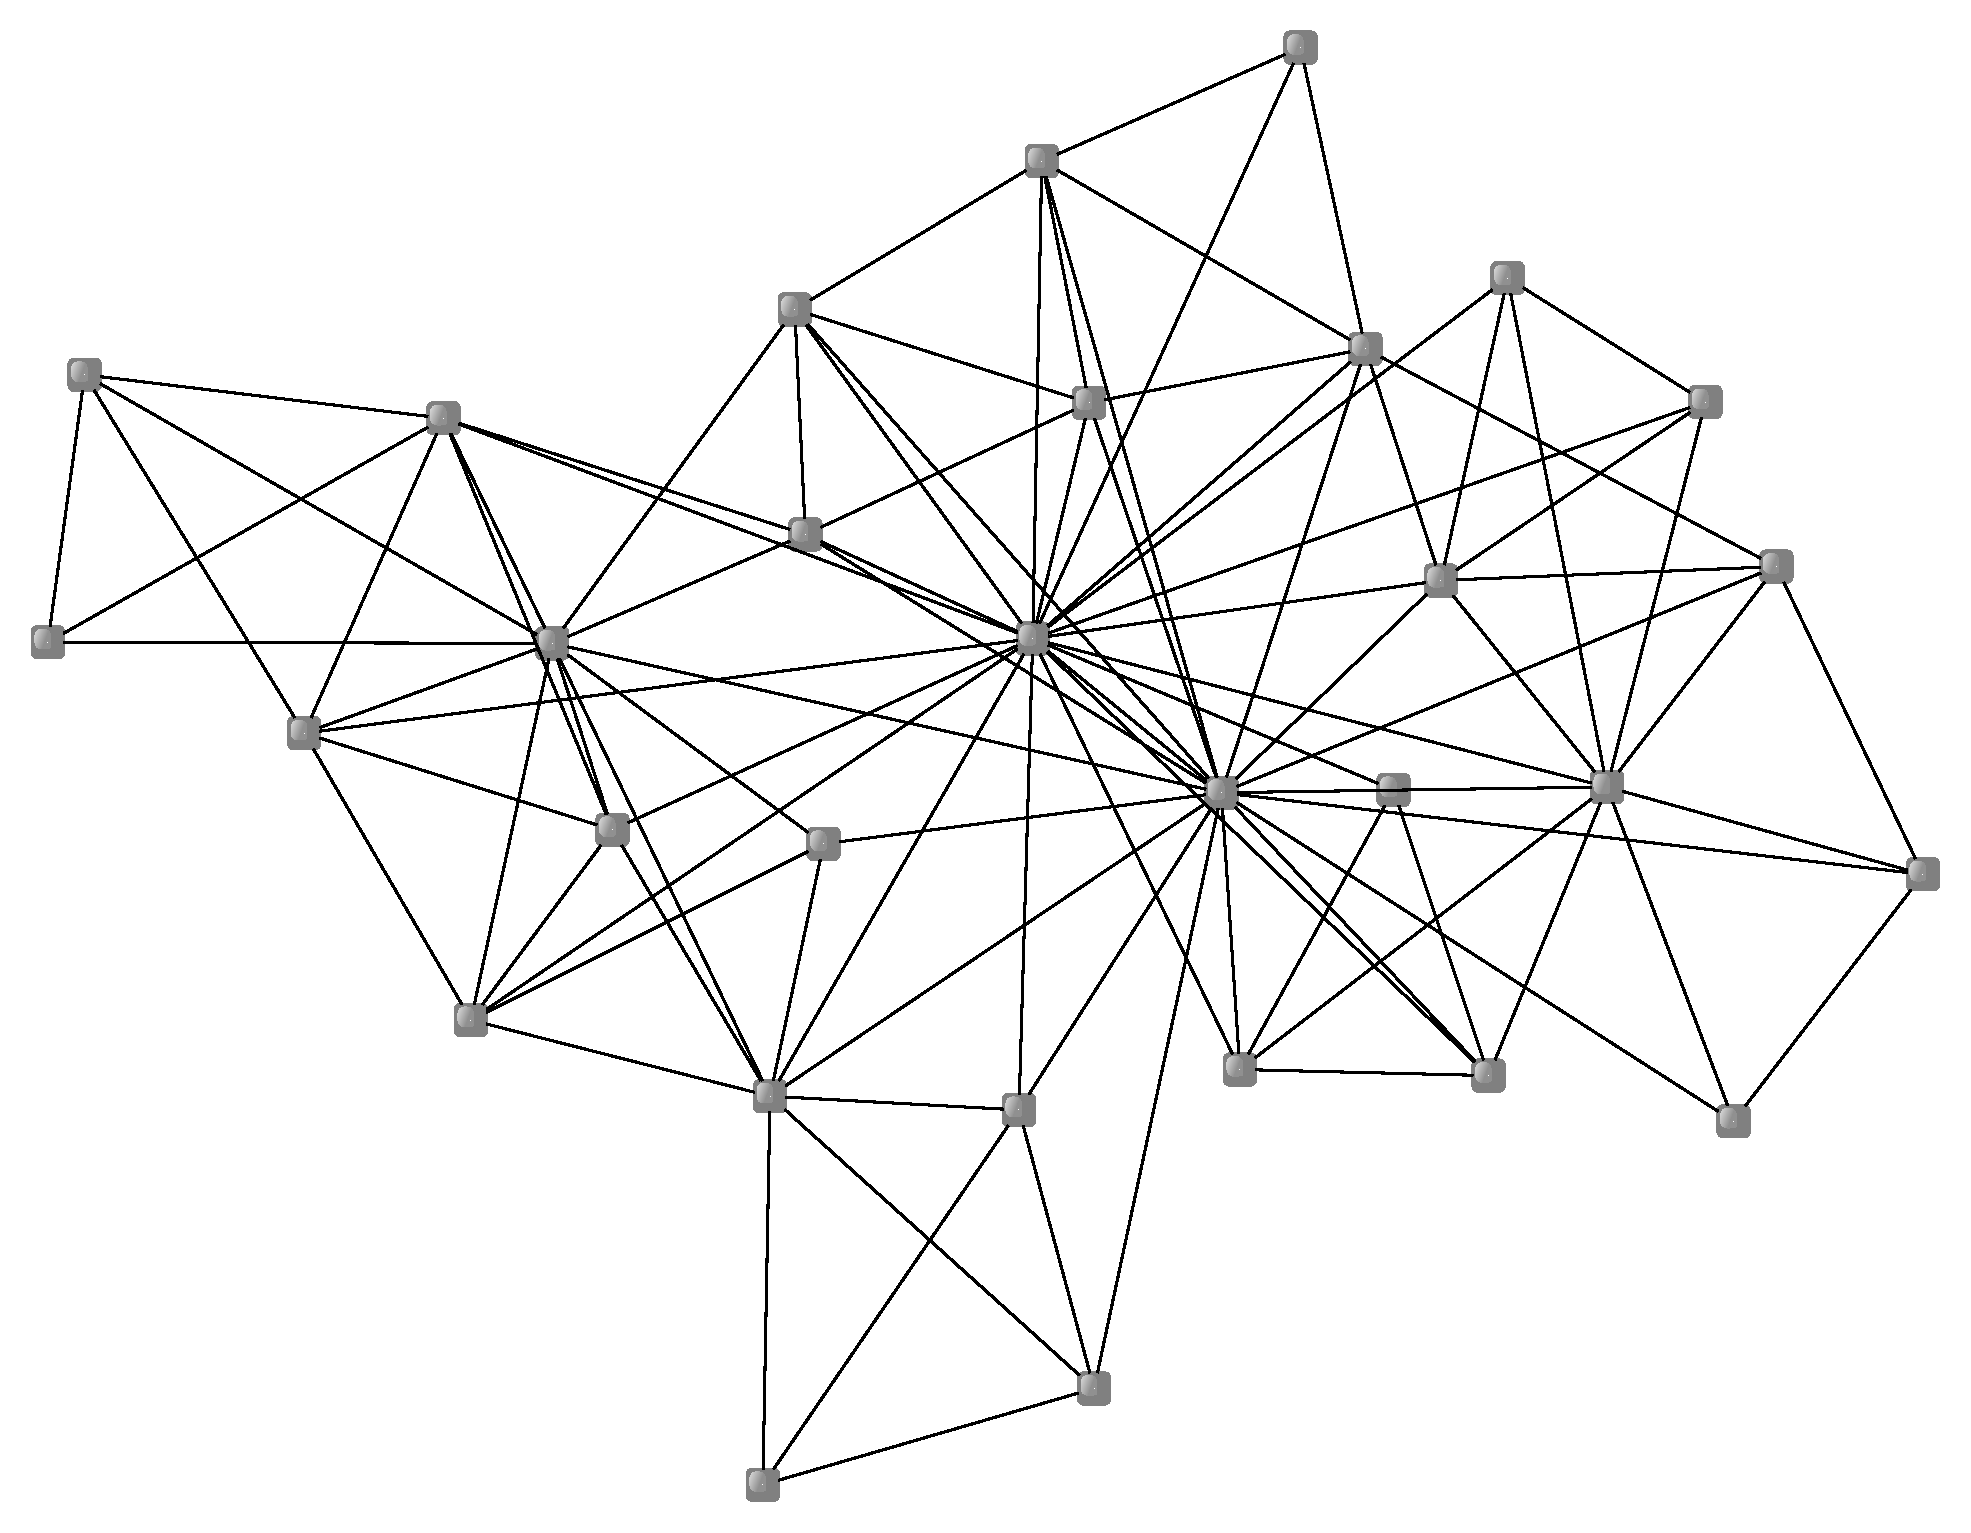
\includegraphics[width=0.27\textwidth]{graph5-huang-angular}}
	\hfill
	\subfloat[\label{fig:graph5-huang-tr}{Total Resolution}]{
	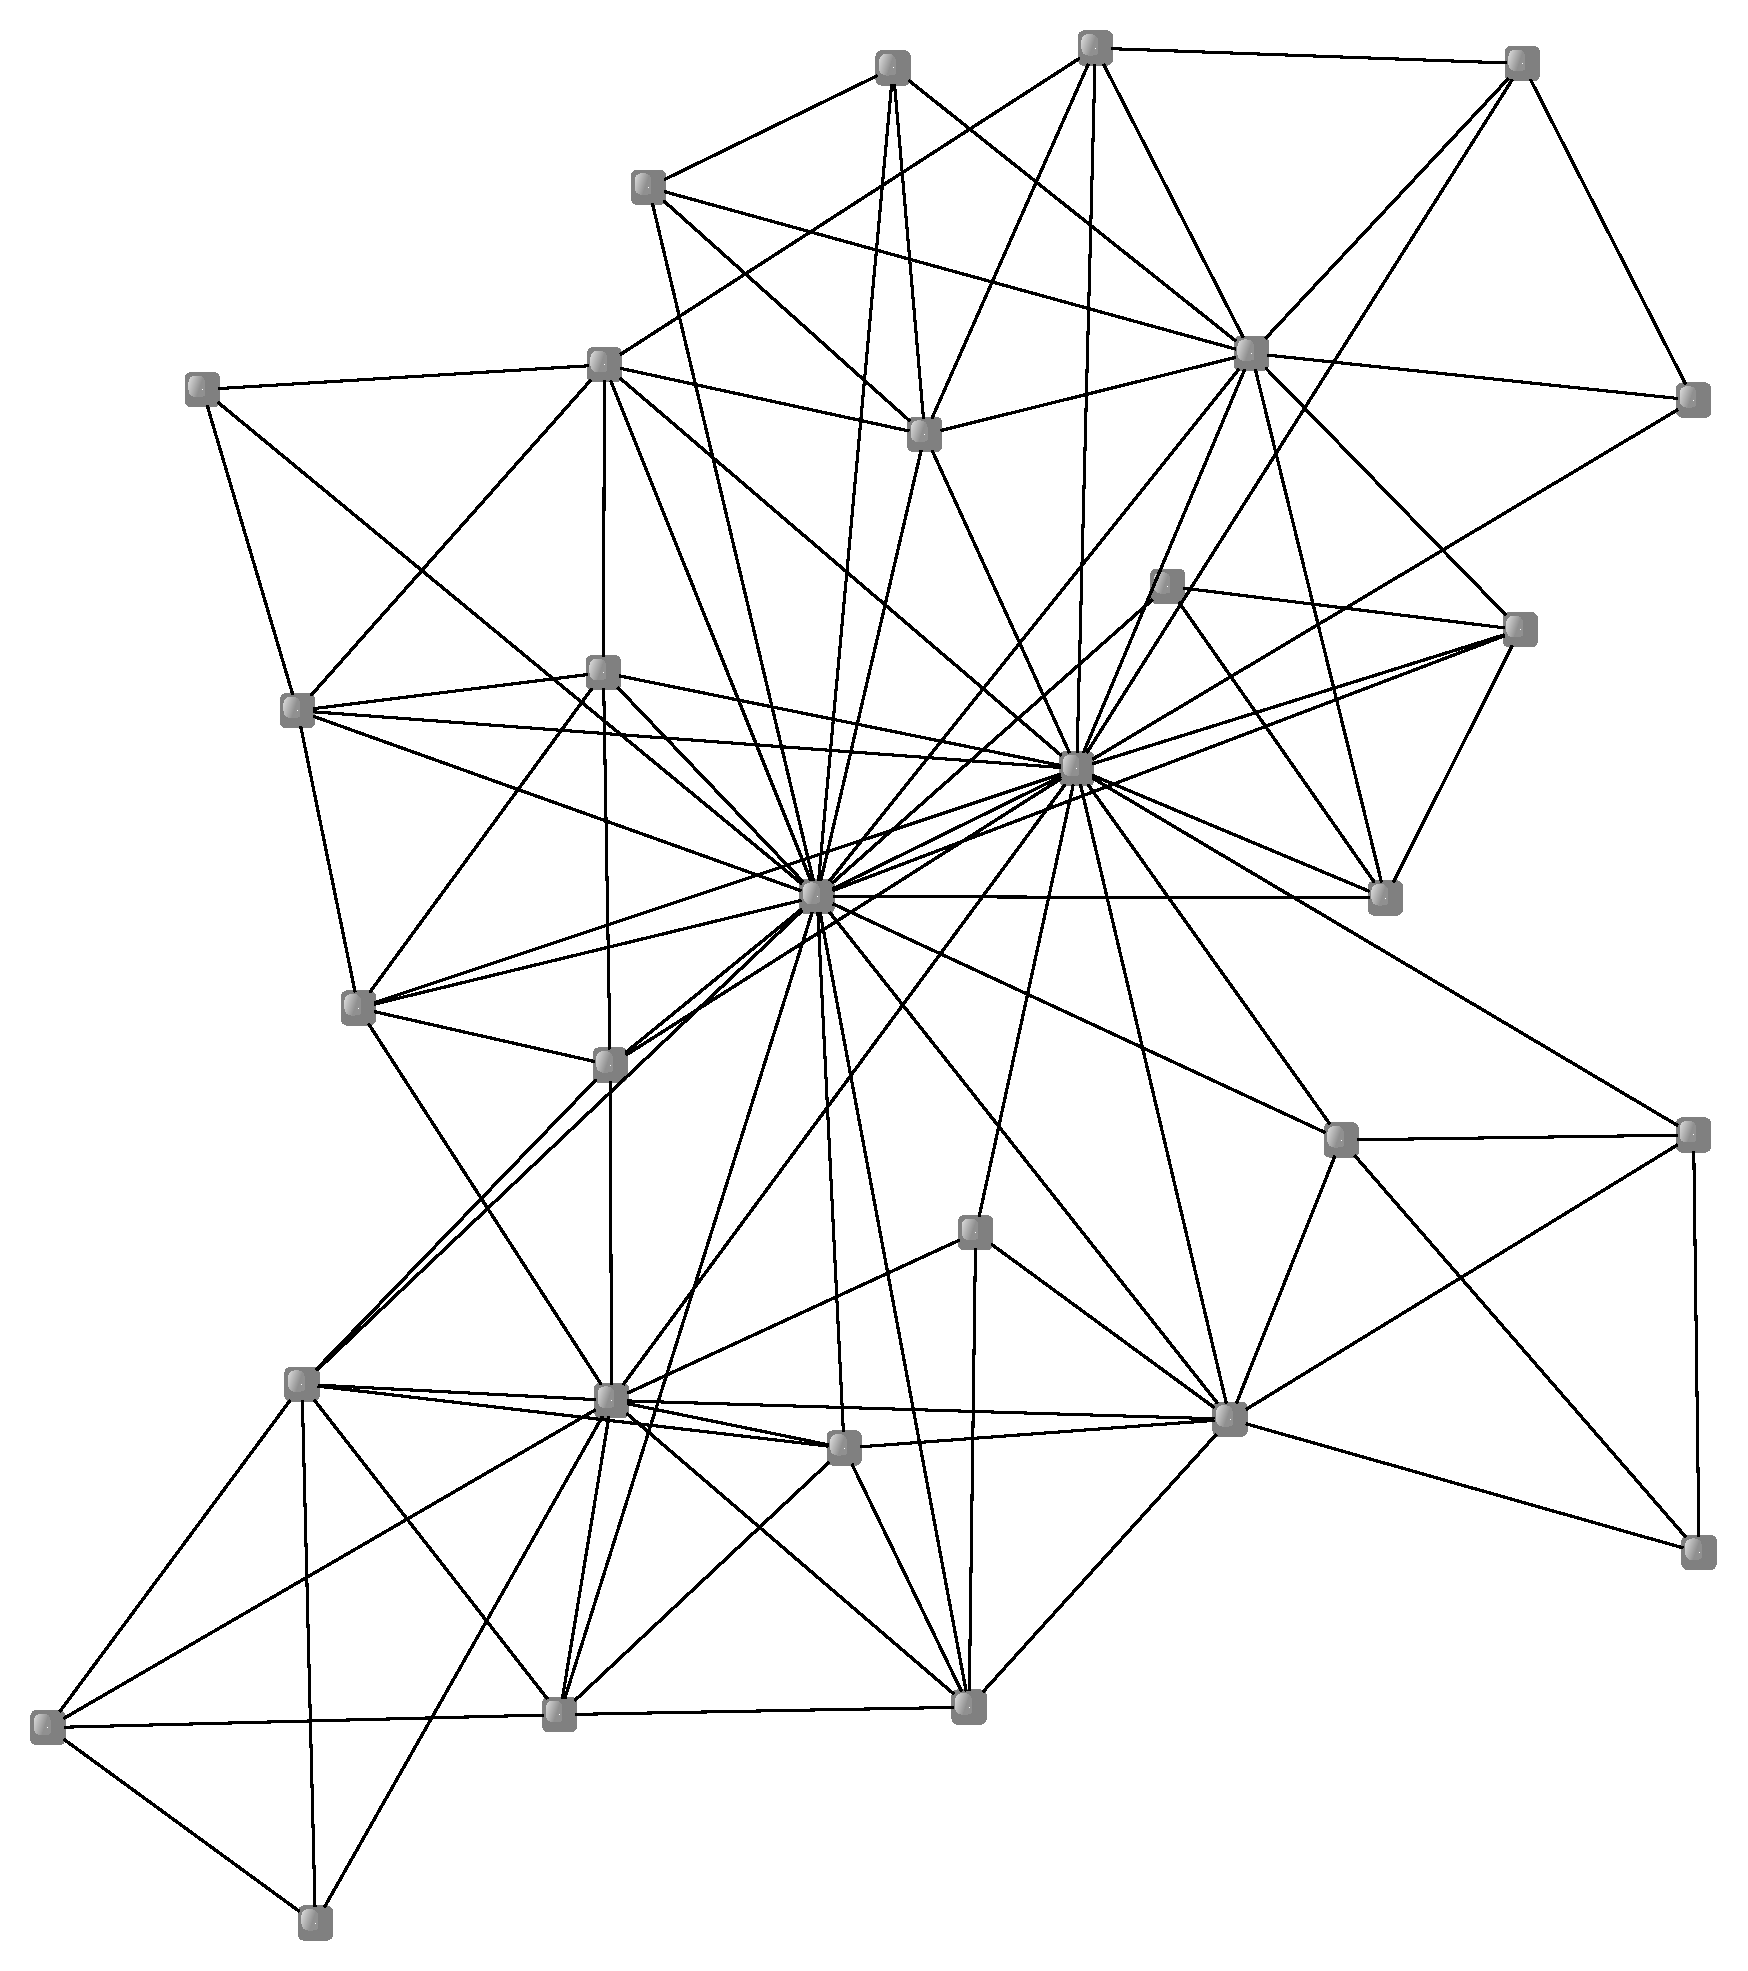
\includegraphics[width=0.27\textwidth]{graph5-huang-total}}
	\caption{Different drawings of the 5th challenge graph given in the Graph Drawing 2017 contest produced by different variants of
	(a)--(c)~the variant of our algorithm without restrictions on the aspect ratio, 
	(d)--(f)~the variant of our algorithm forced to maintain the input aspect ratio,
	(g)--(i)~the algorithm by Argyriou et al.~\cite{DBLP:journals/cj/ArgyriouBS13}, and
	(j)--(l)~the algorithm by Huang et al.~\cite{DBLP:journals/vlc/HuangEHL13}.
	The aesthetic criterion optimized by each variant is reported in the caption of its subfigure.}
	\label{fig:graph5}
\end{figure*}

\begin{figure*}[htbp]
	\centering
	\subfloat[\label{fig:graph9-ourBest-cr}{Crossing Resolution}]{
	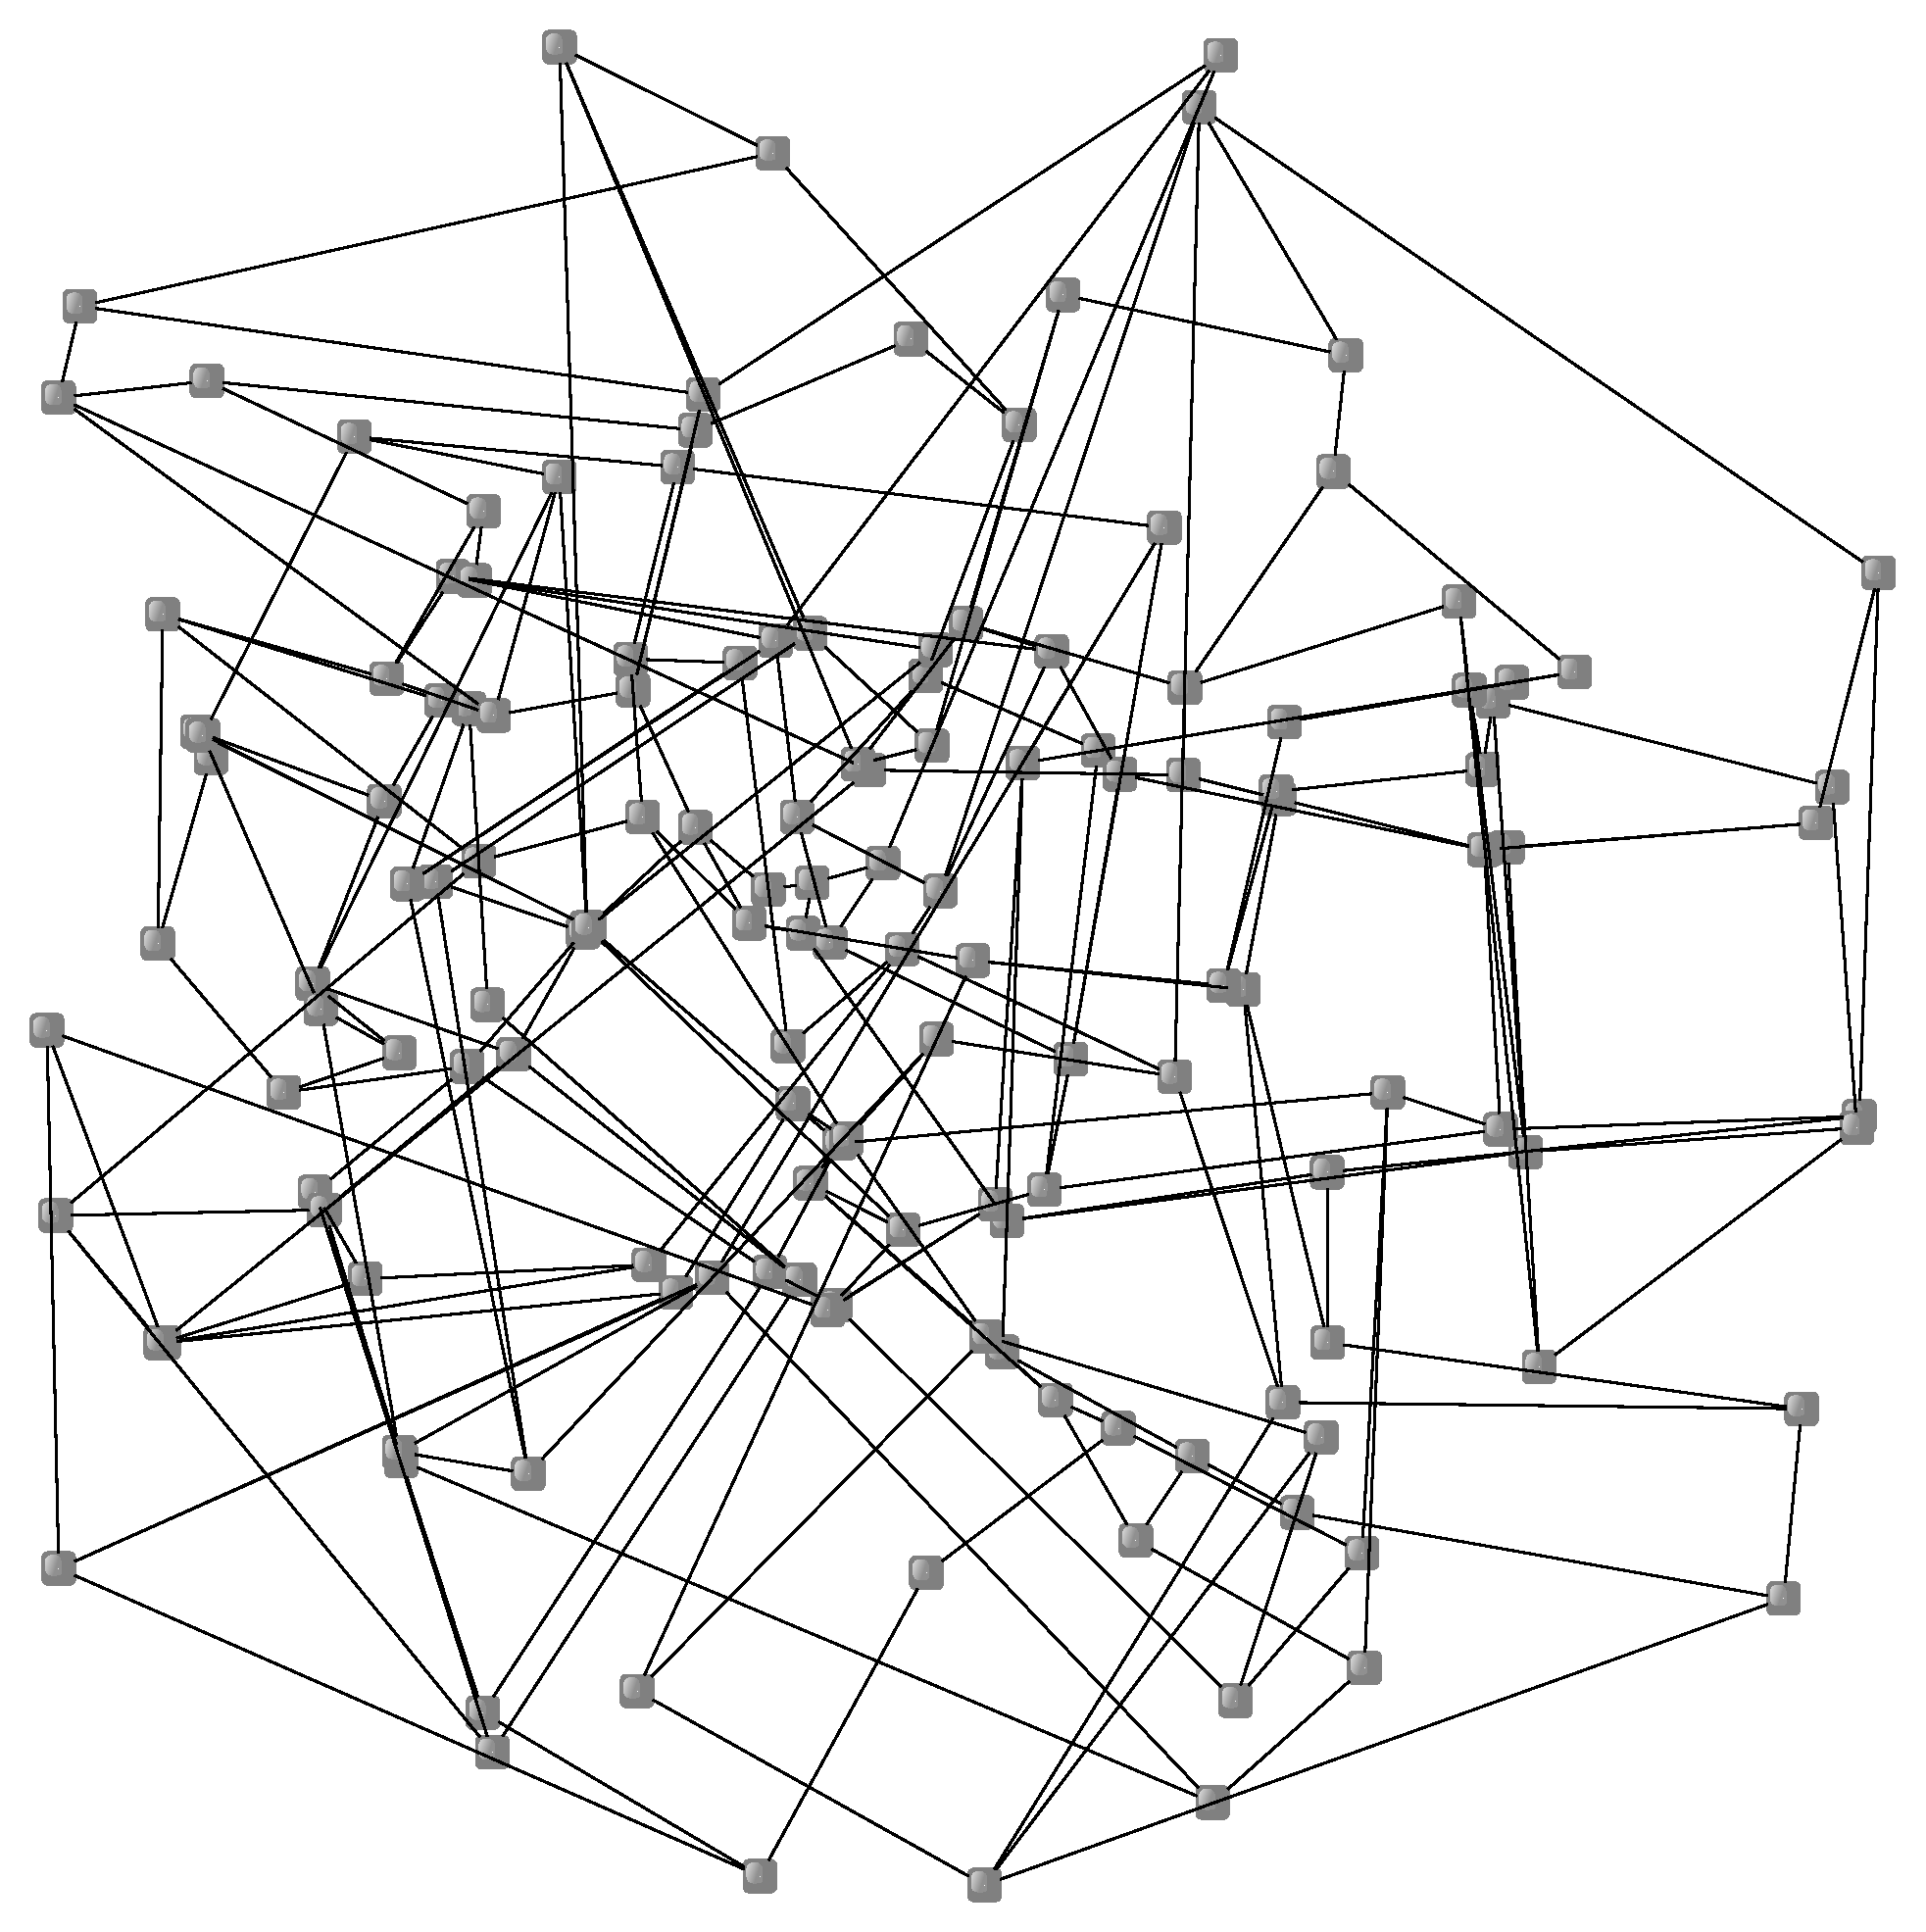
\includegraphics[width=0.27\textwidth]{graph9-ourBest-crossing}}
	\hfill
	\subfloat[\label{fig:graph9-ourBest-ar}{Angular Resolution}]{
	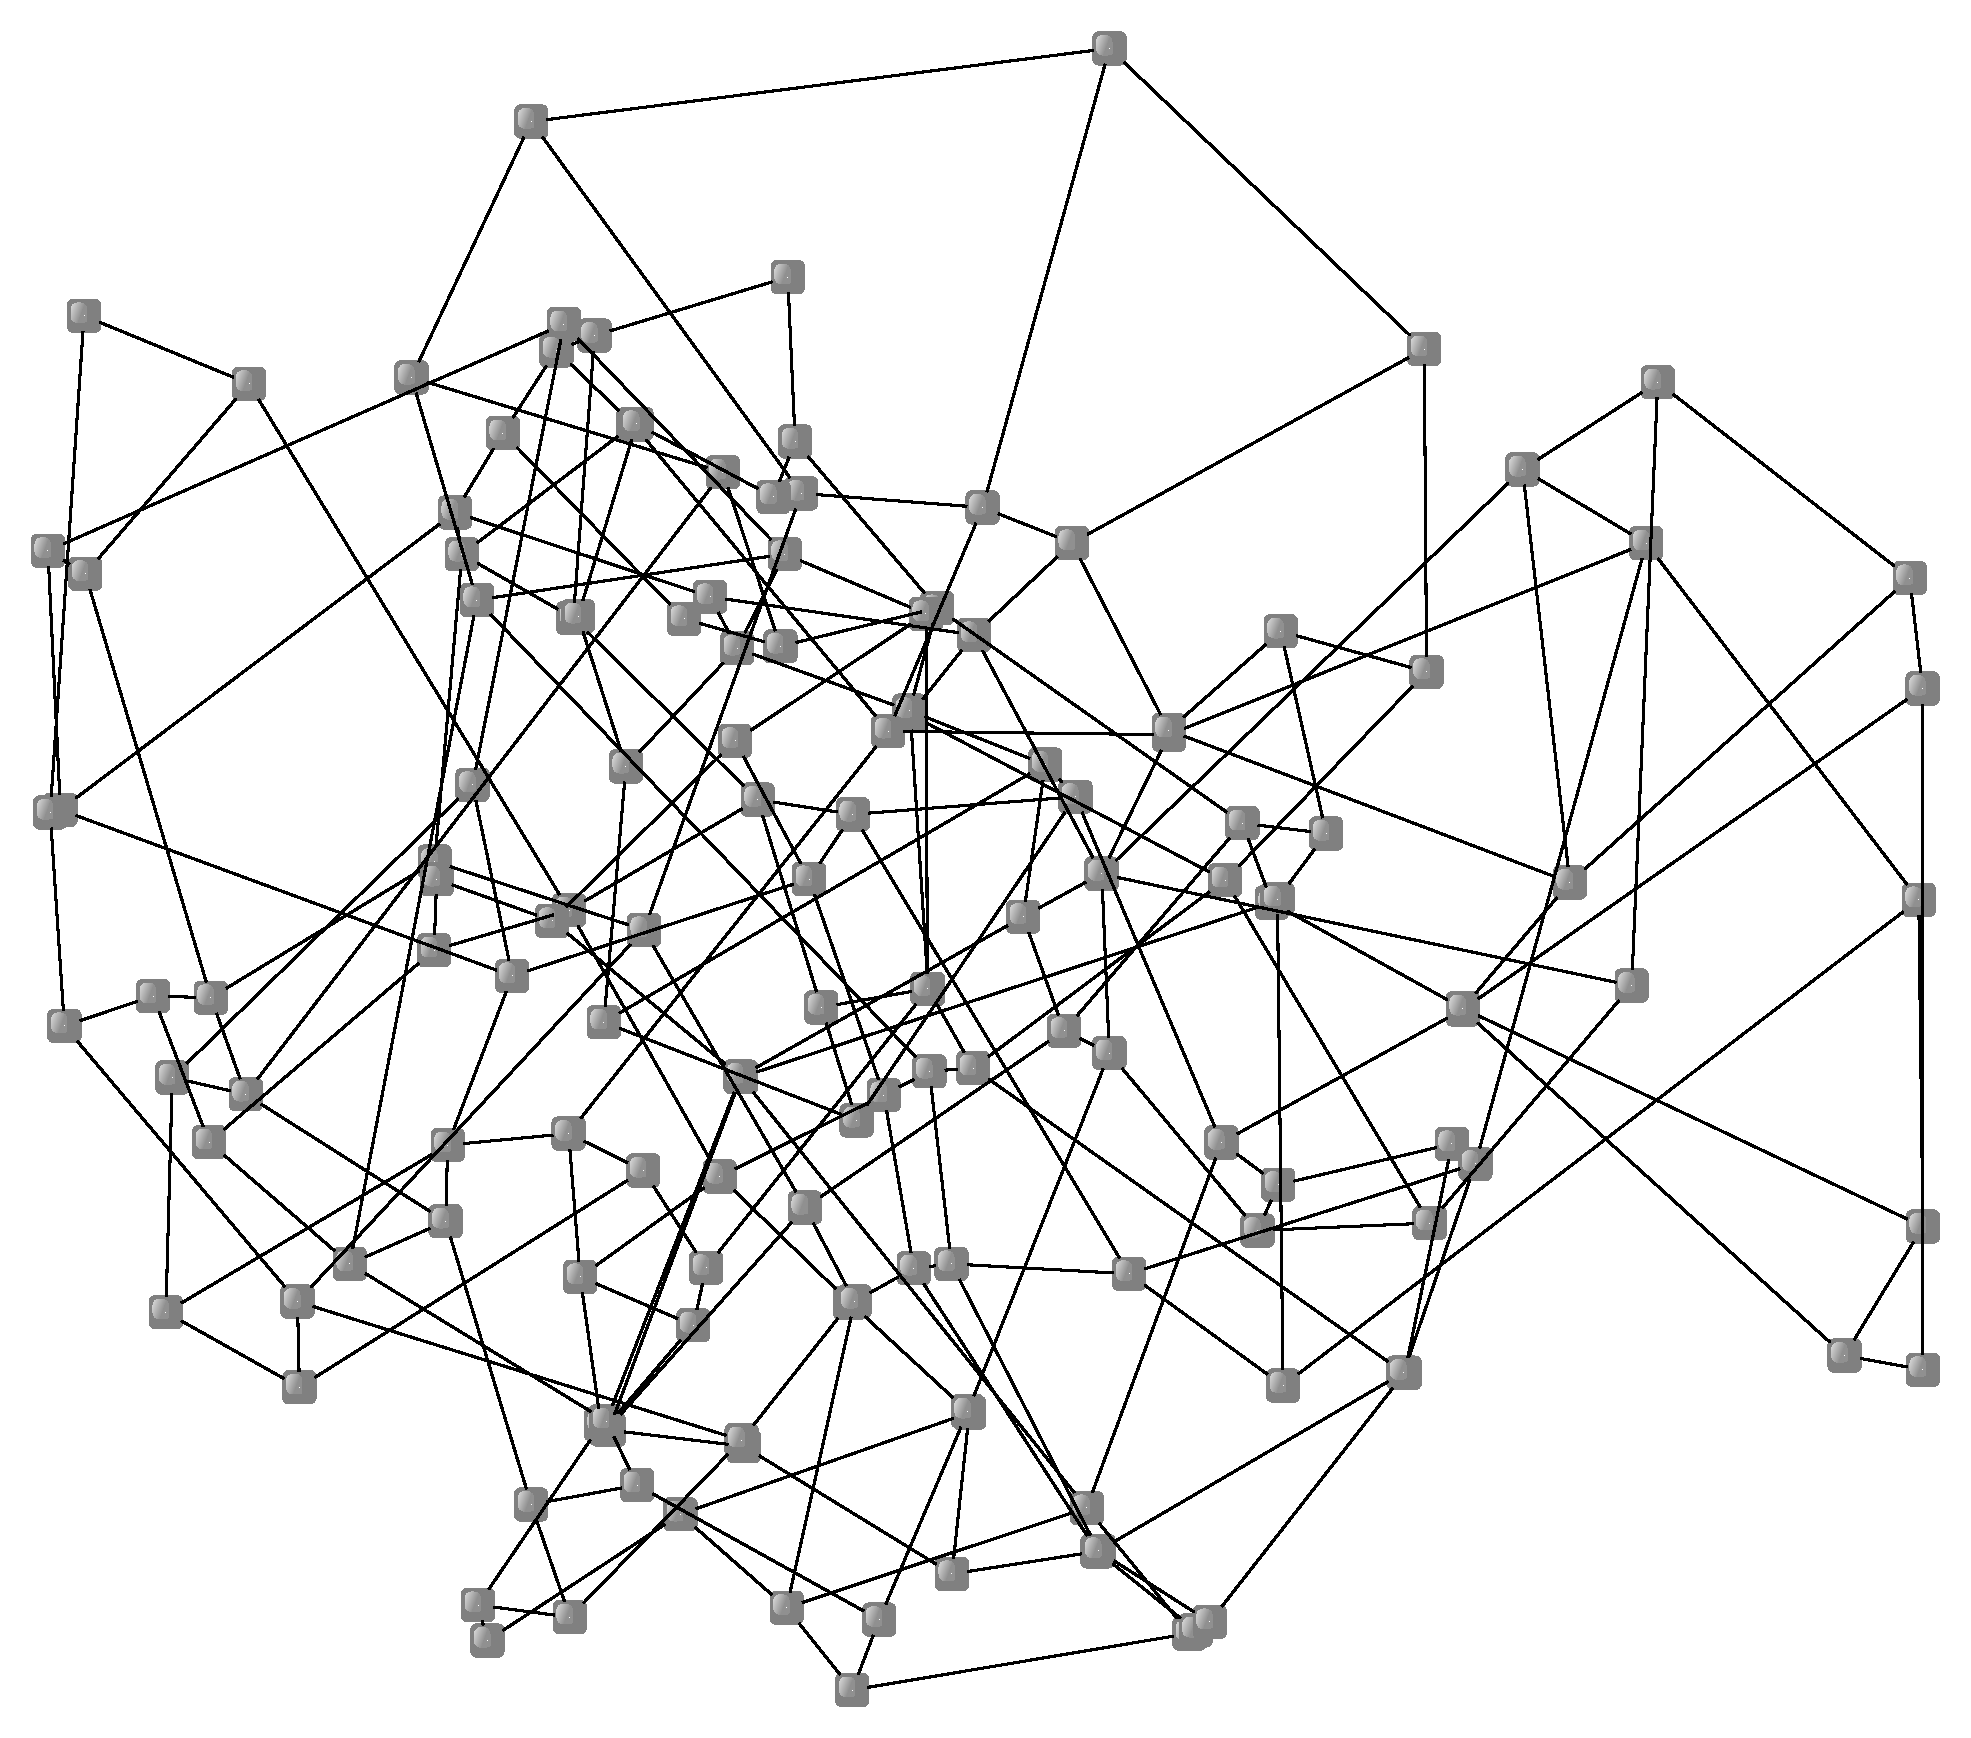
\includegraphics[width=0.27\textwidth]{graph9-ourBest-angular}}
	\hfill
	\subfloat[\label{fig:graph9-ourBest-tr}{Total Resolution}]{
	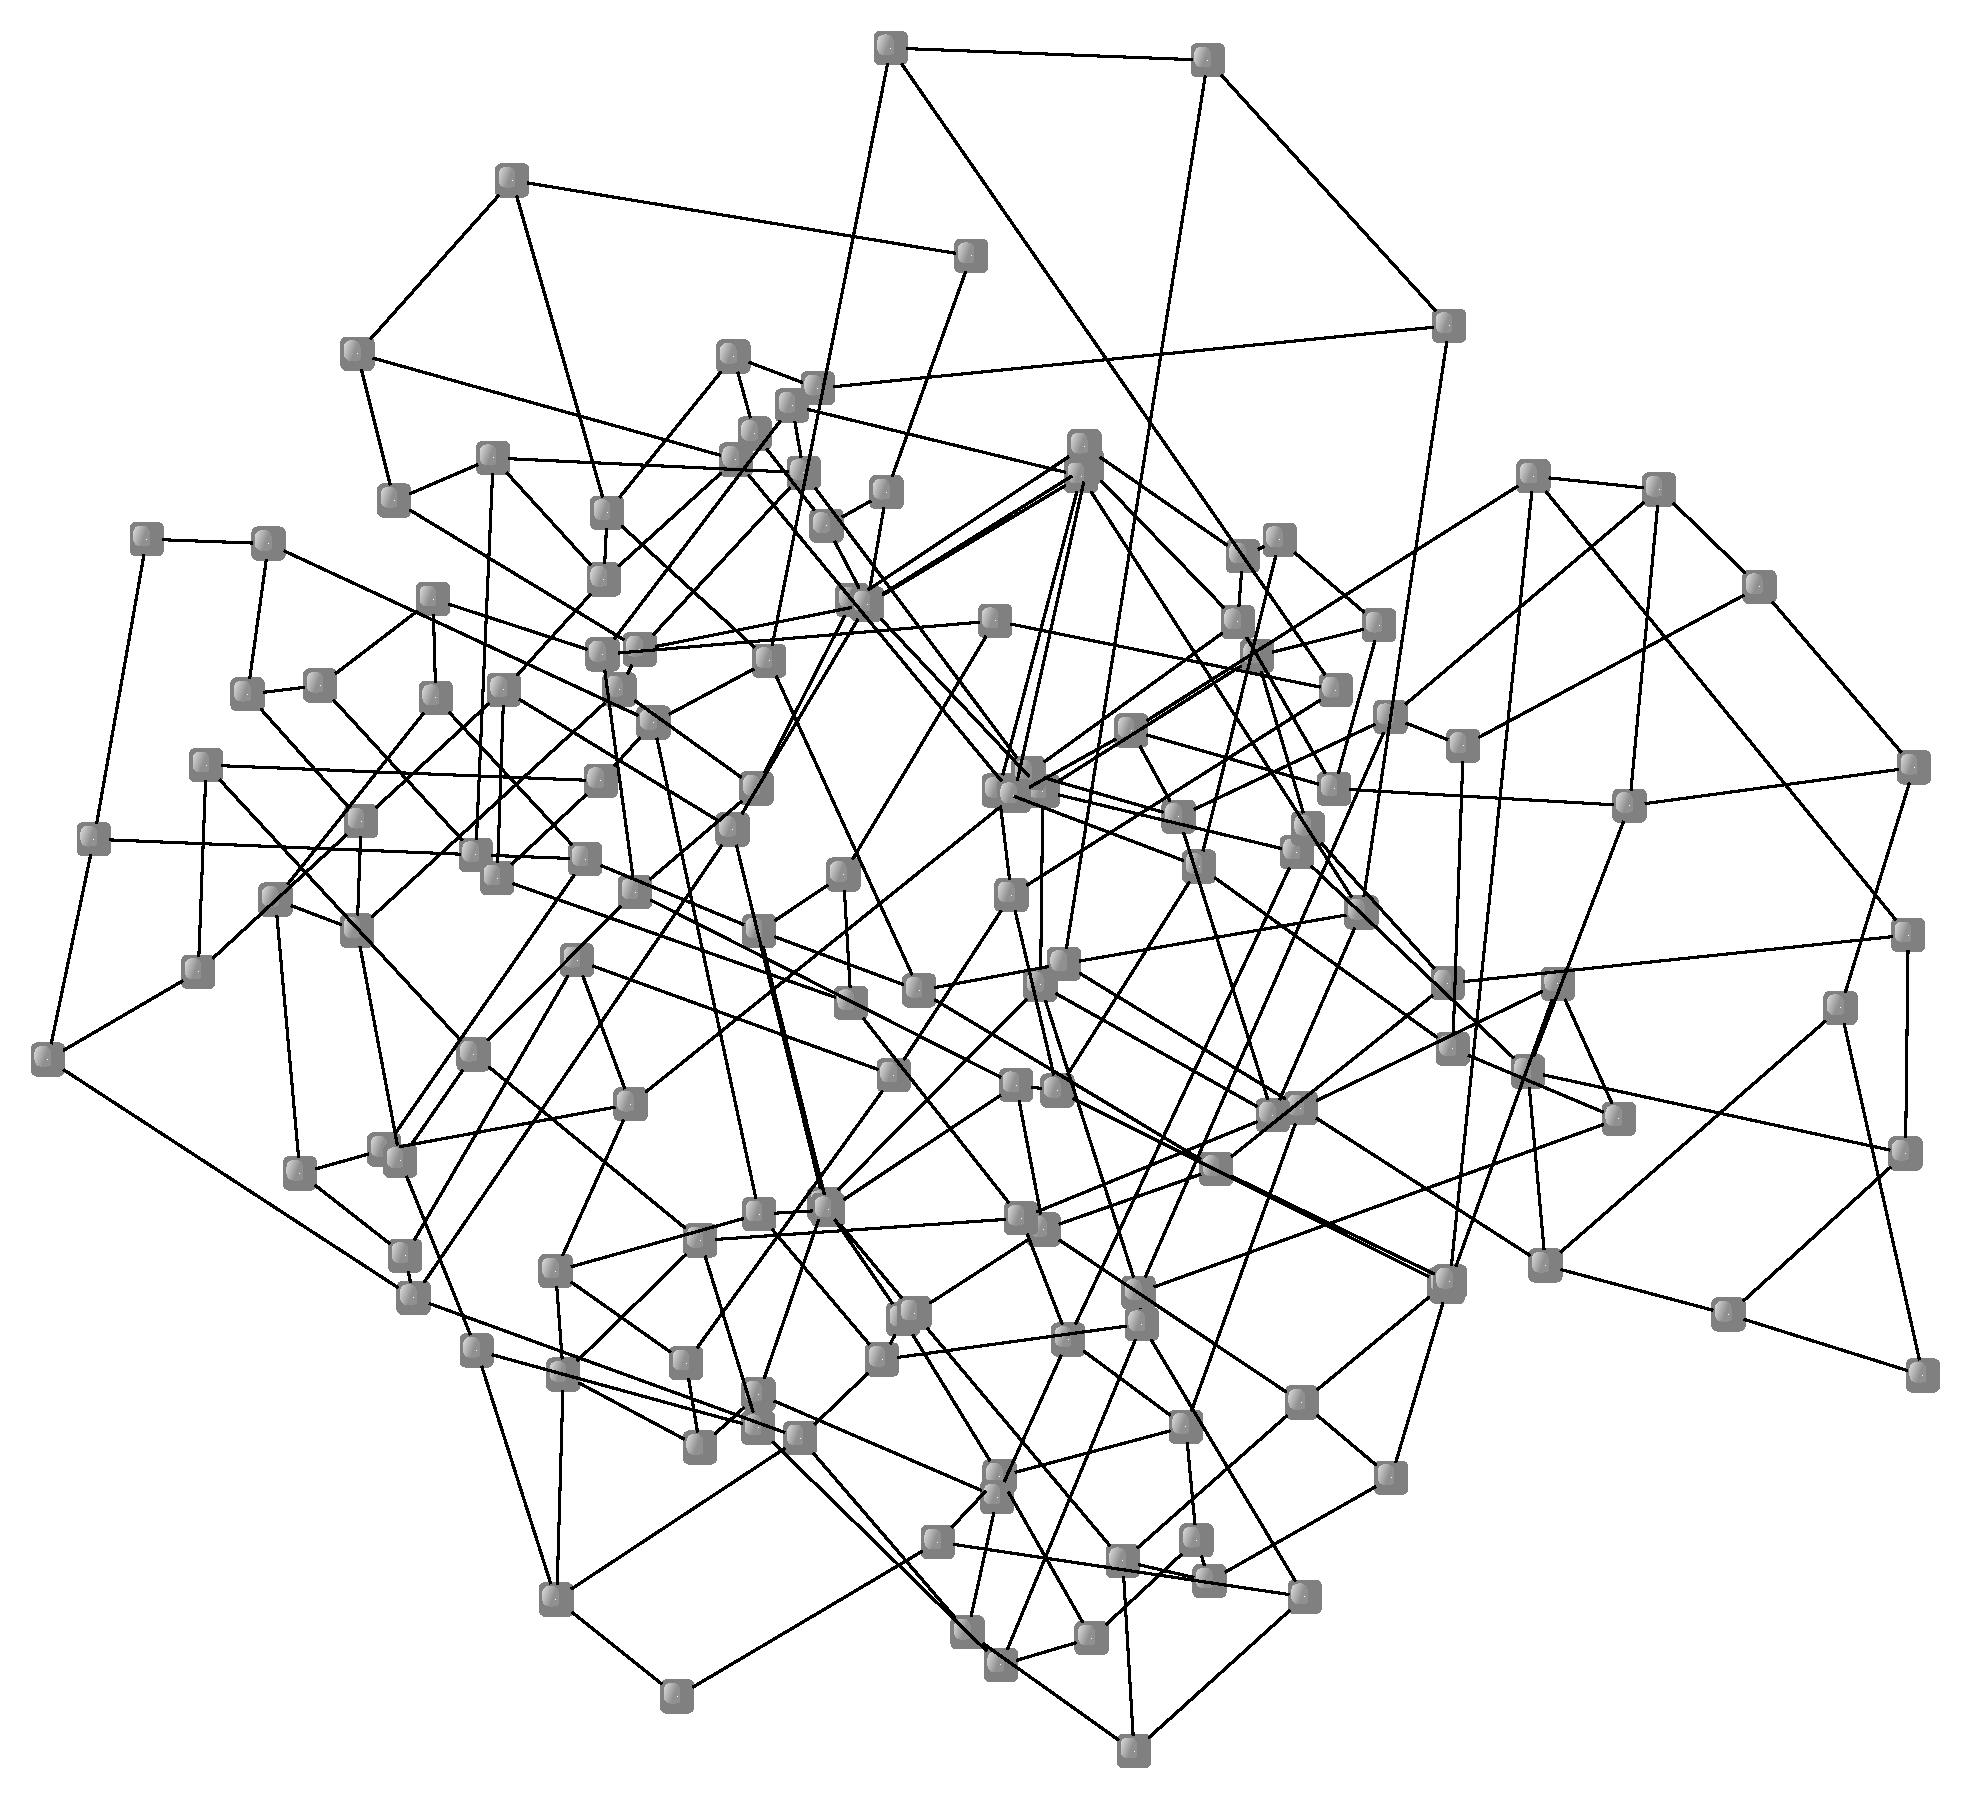
\includegraphics[width=0.27\textwidth]{graph9-ourBest-total}}
	\hfill	
	\subfloat[\label{fig:graph9-ourRestricted-cr}{Crossing Resolution}]{
	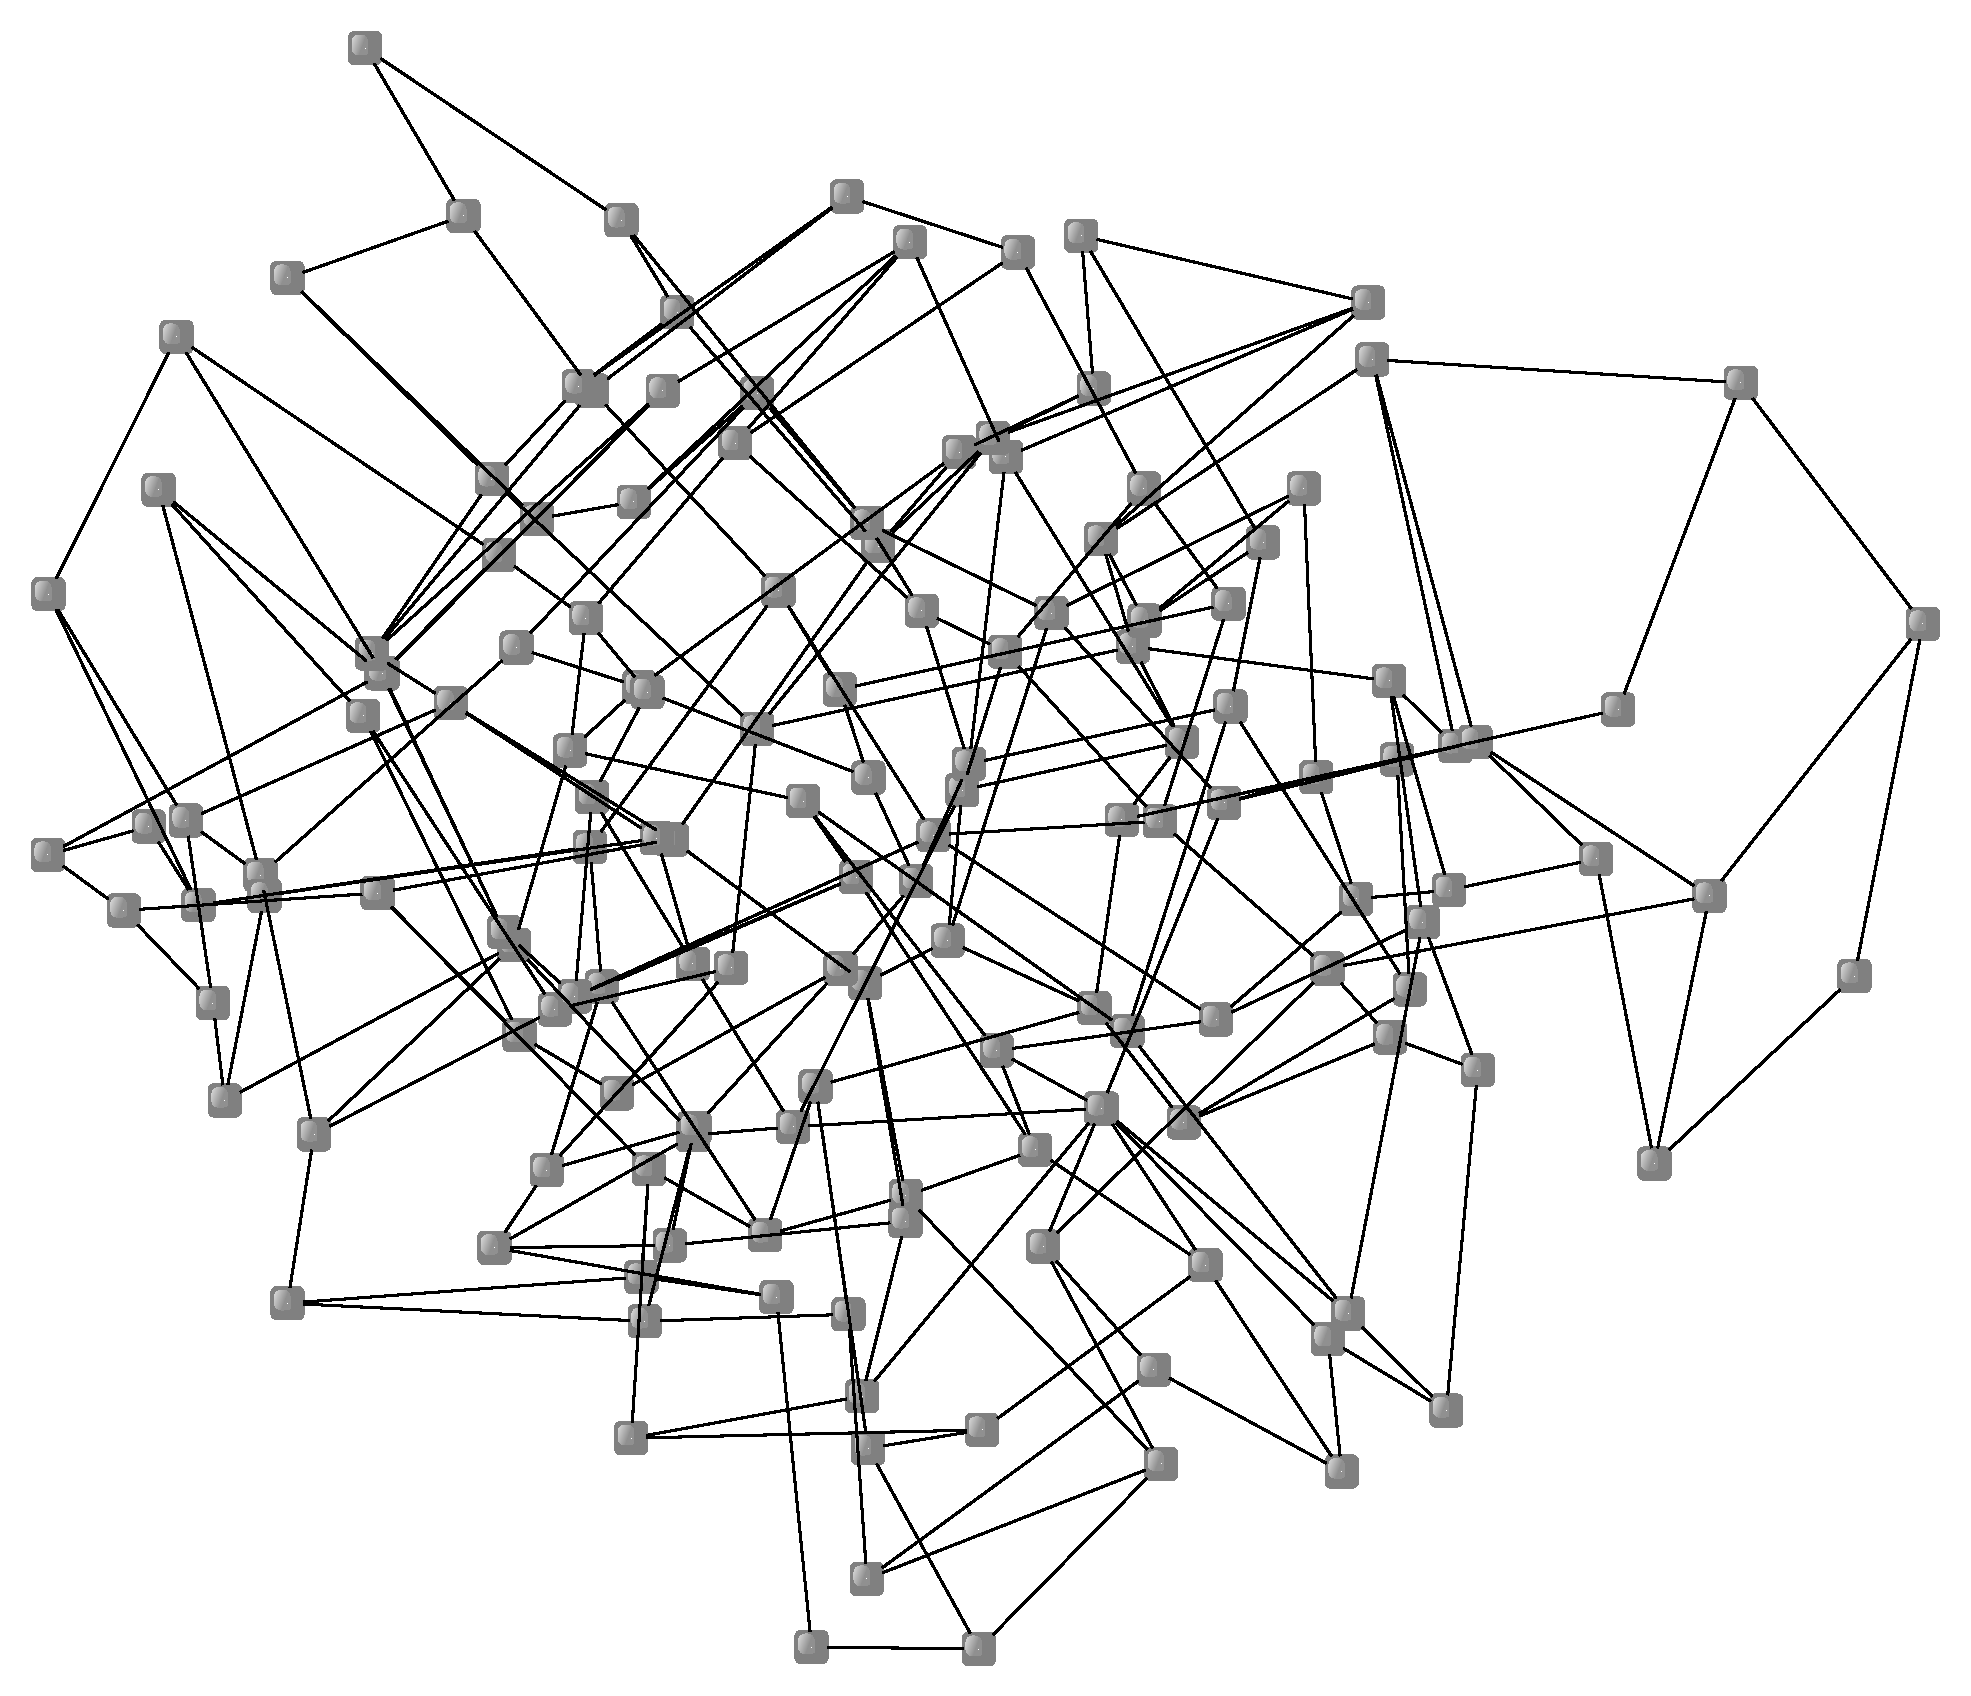
\includegraphics[width=0.27\textwidth]{graph9-ourRestricted-crossing}}
	\hfill
	\subfloat[\label{fig:graph9-ourRestricted-ar}{Angular Resolution}]{
	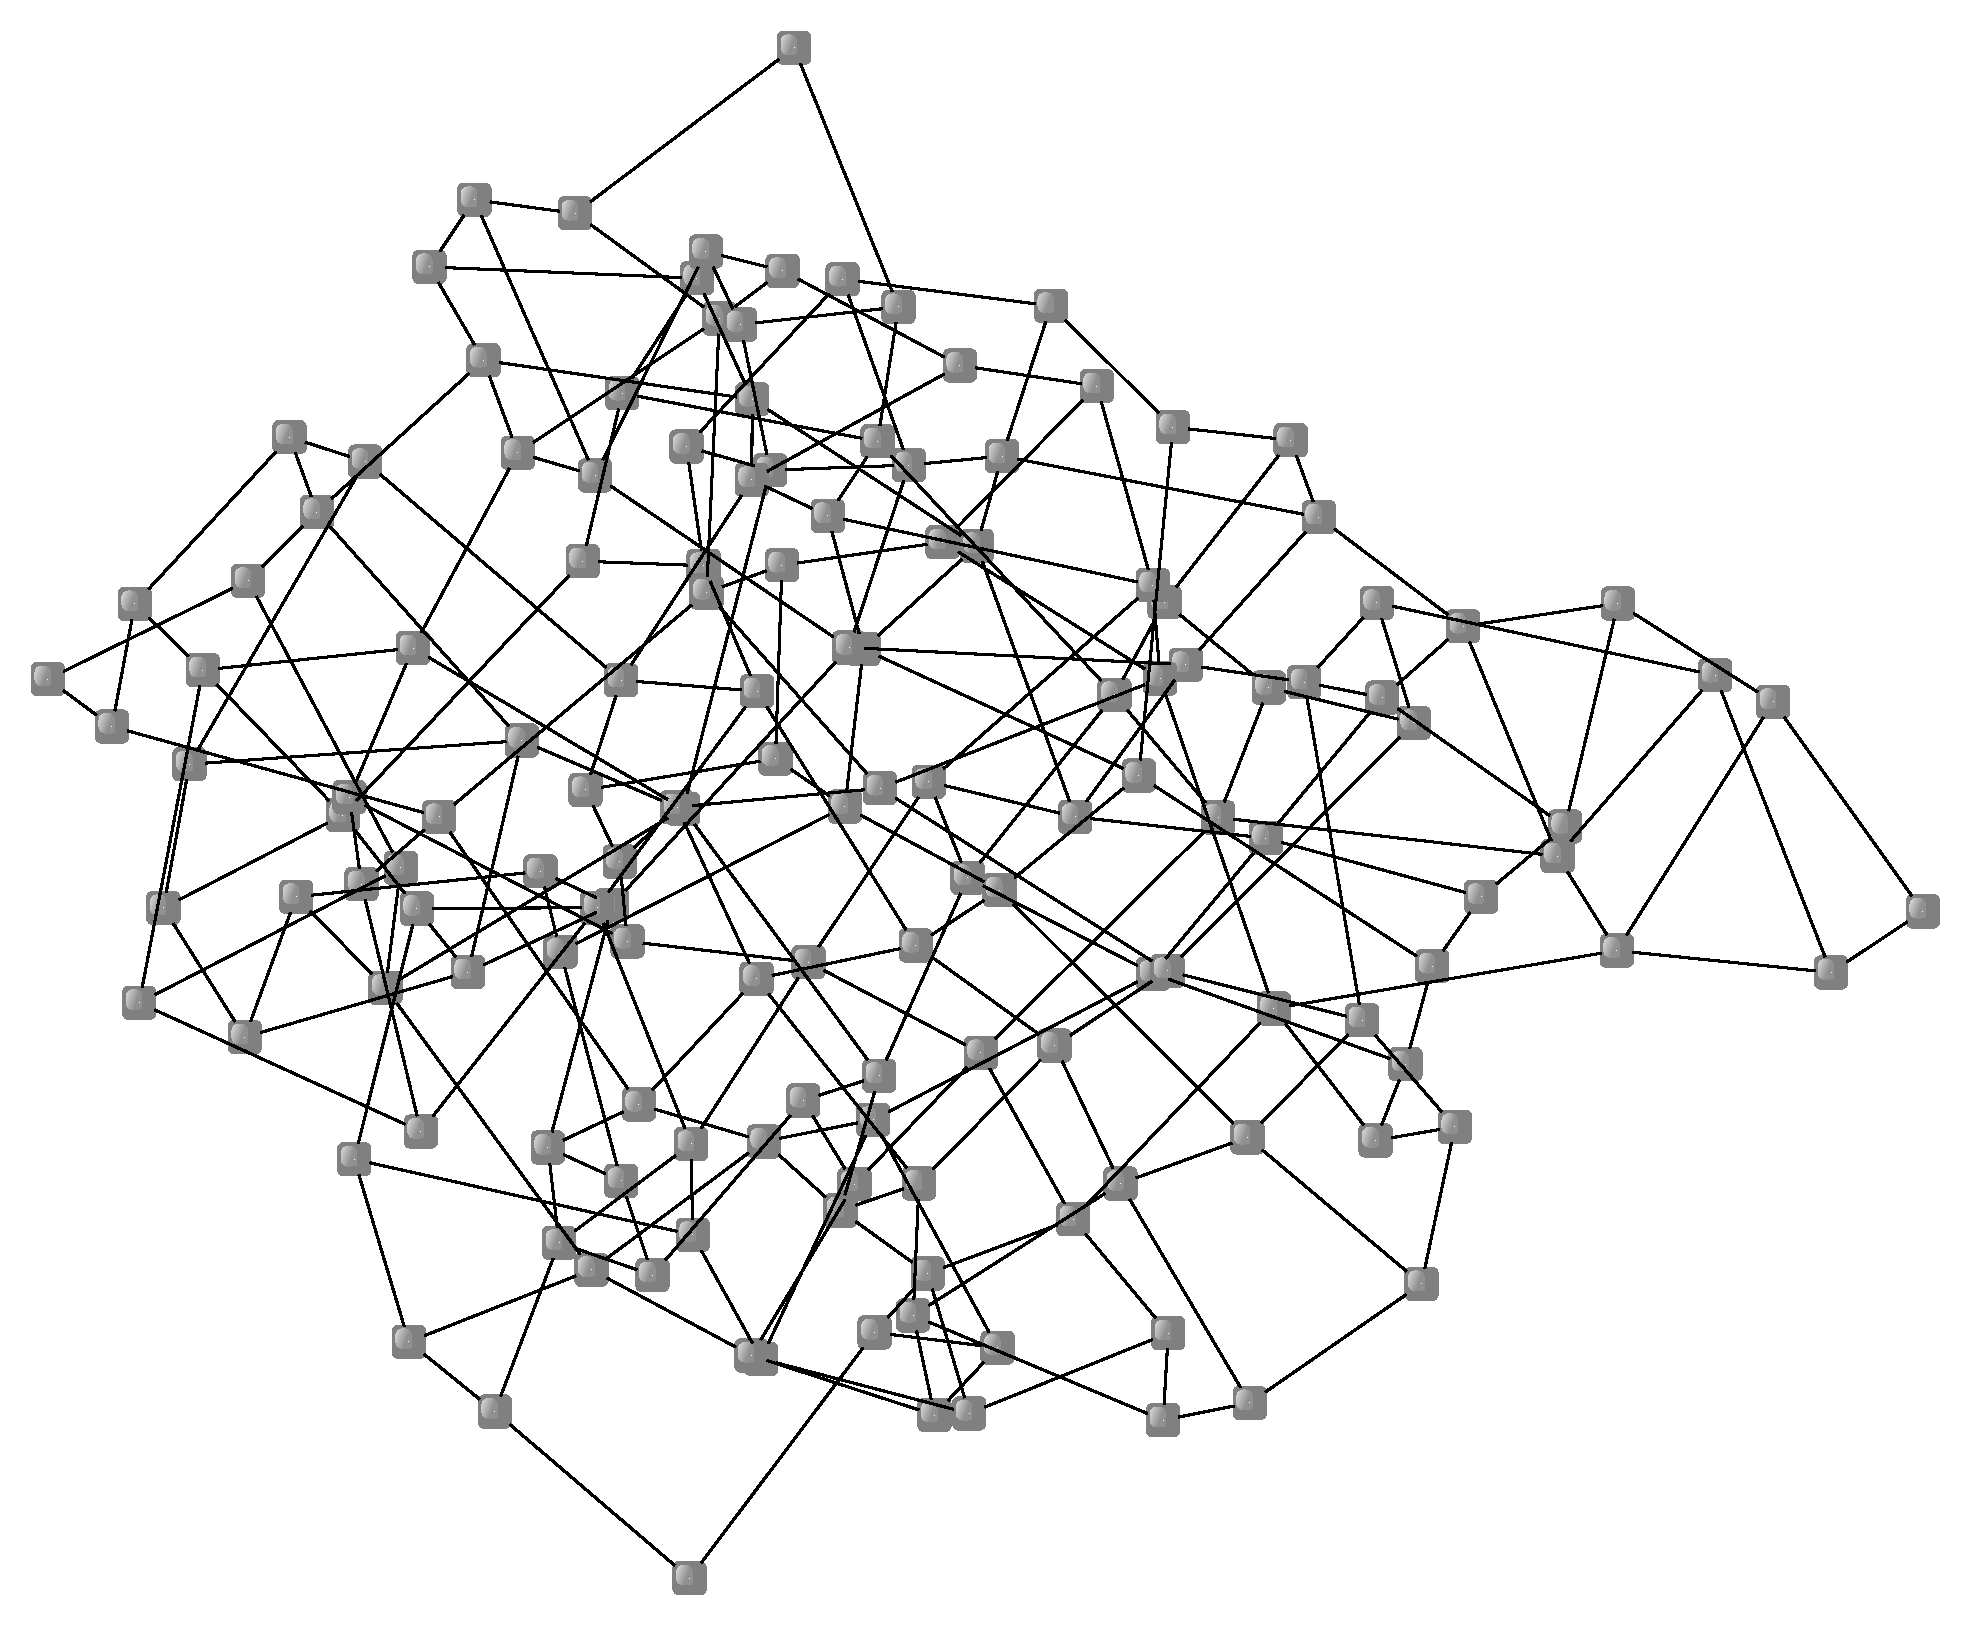
\includegraphics[width=0.27\textwidth]{graph9-ourRestricted-angular}}
	\hfill
	\subfloat[\label{fig:graph9-ourRestricted-tr}{Total Resolution}]{
	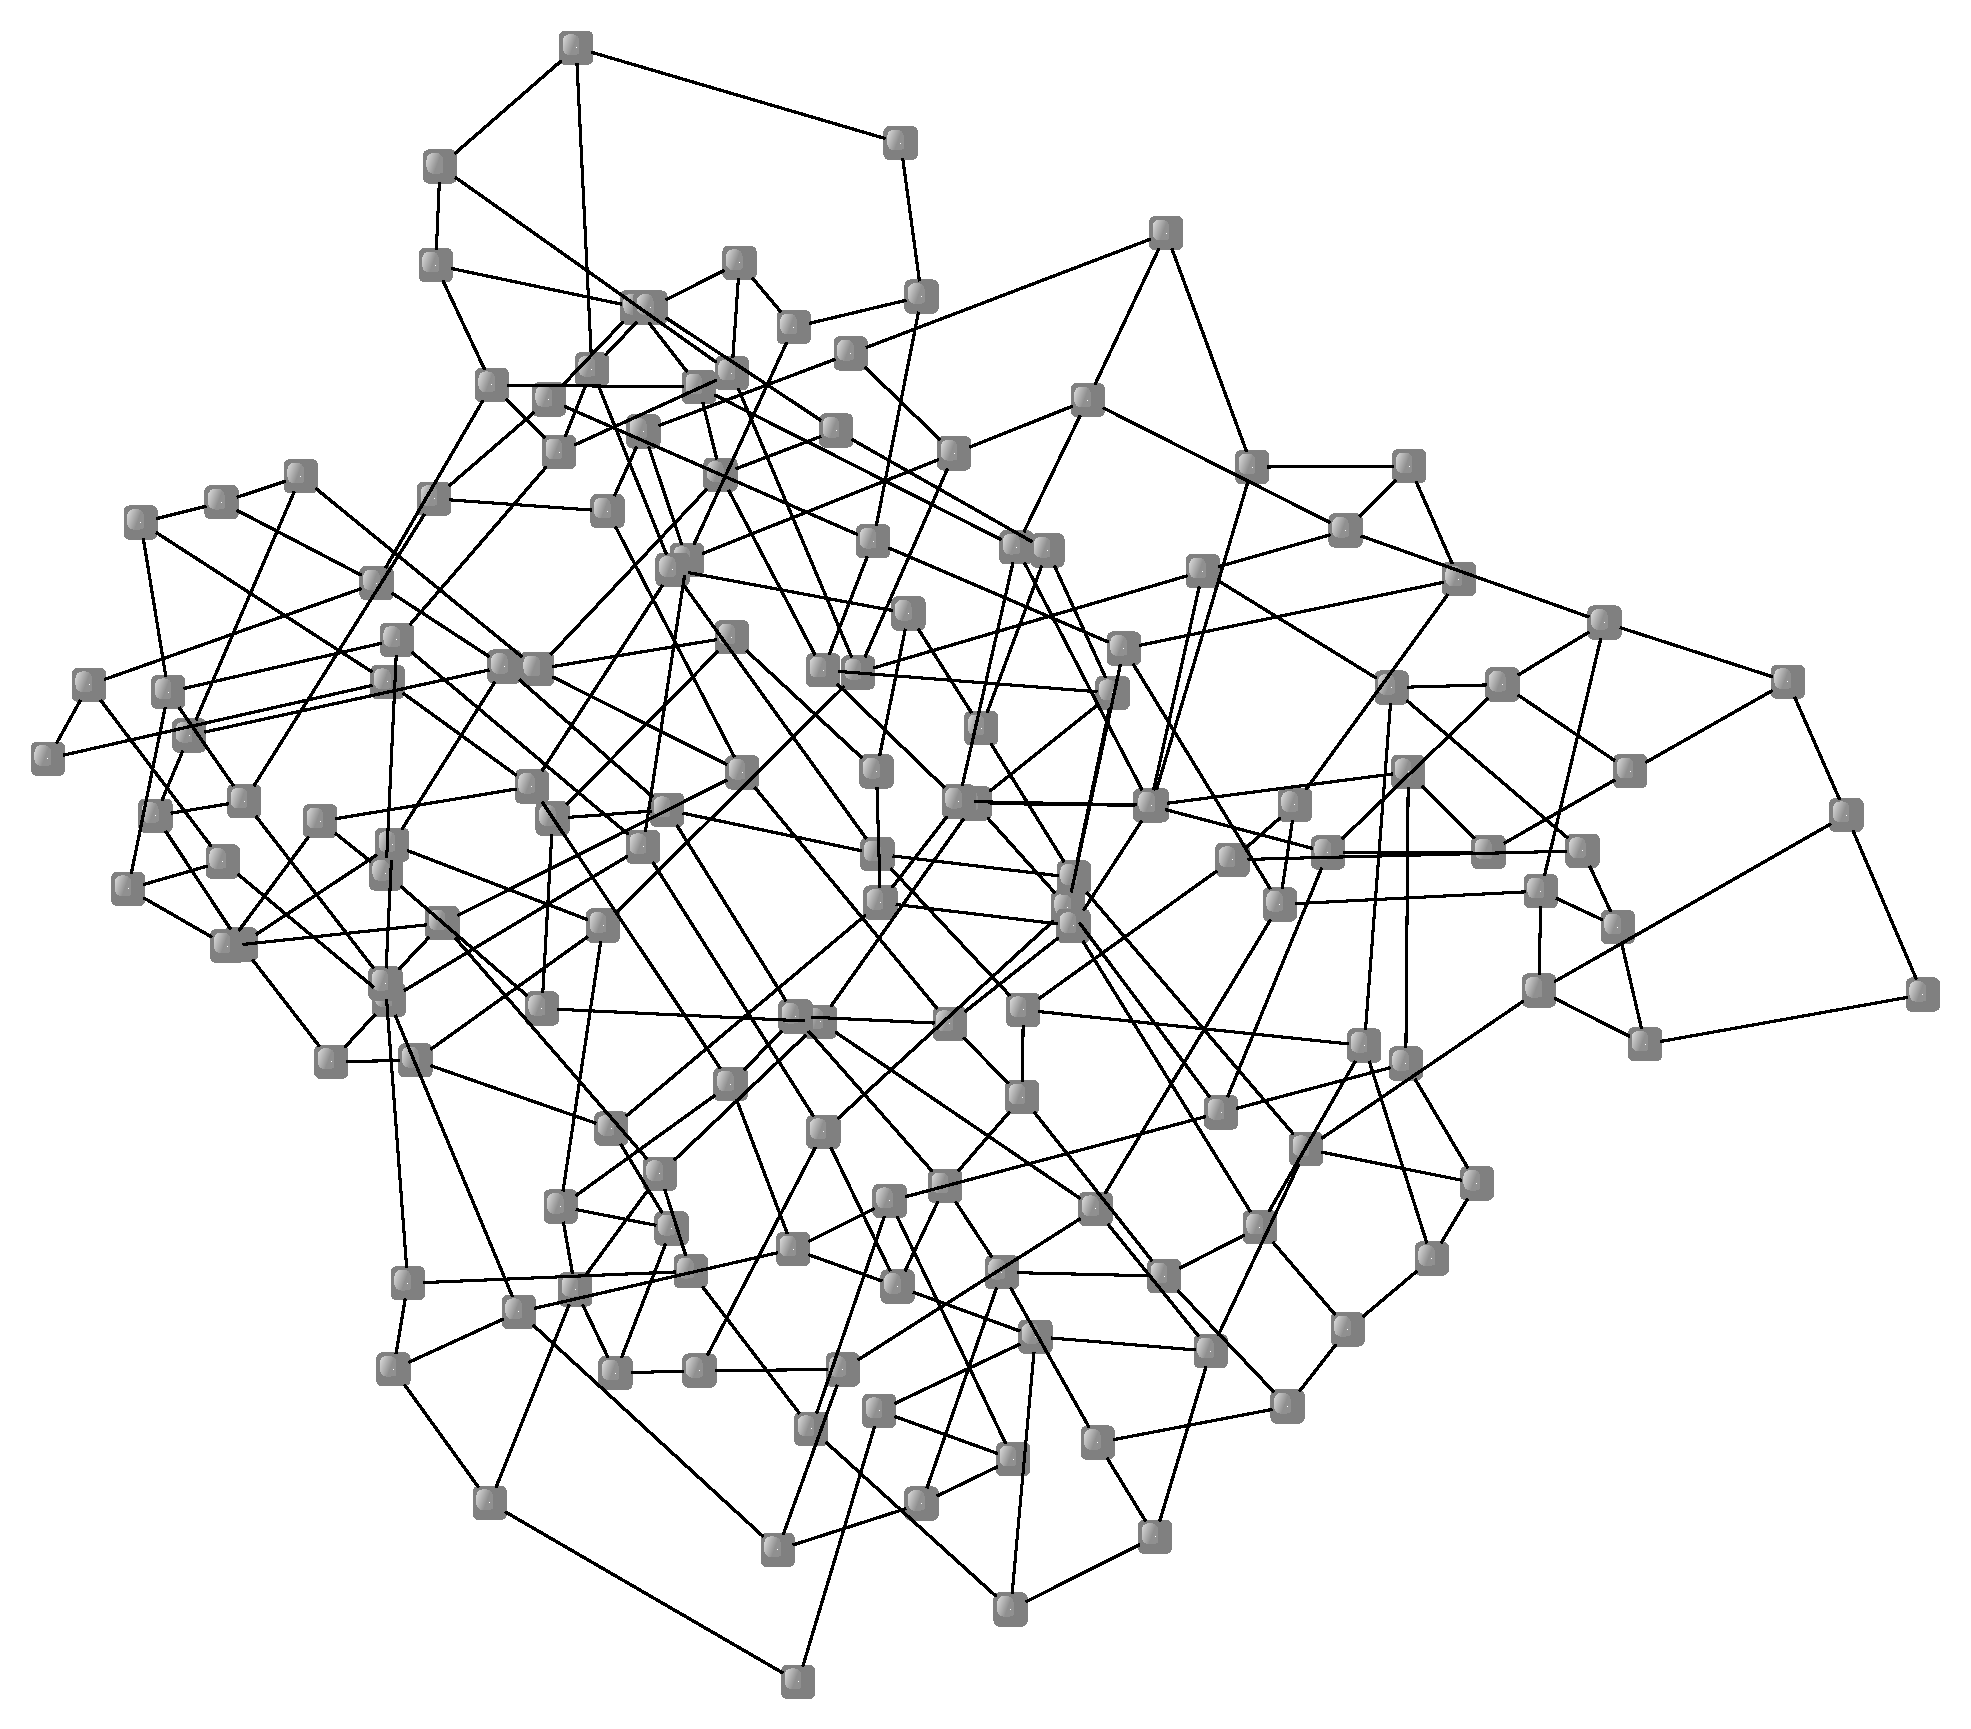
\includegraphics[width=0.27\textwidth]{graph9-ourRestricted-total}}	
	\hfill	
	\subfloat[\label{fig:graph9-argyriou-cr}{Crossing Resolution}]{
	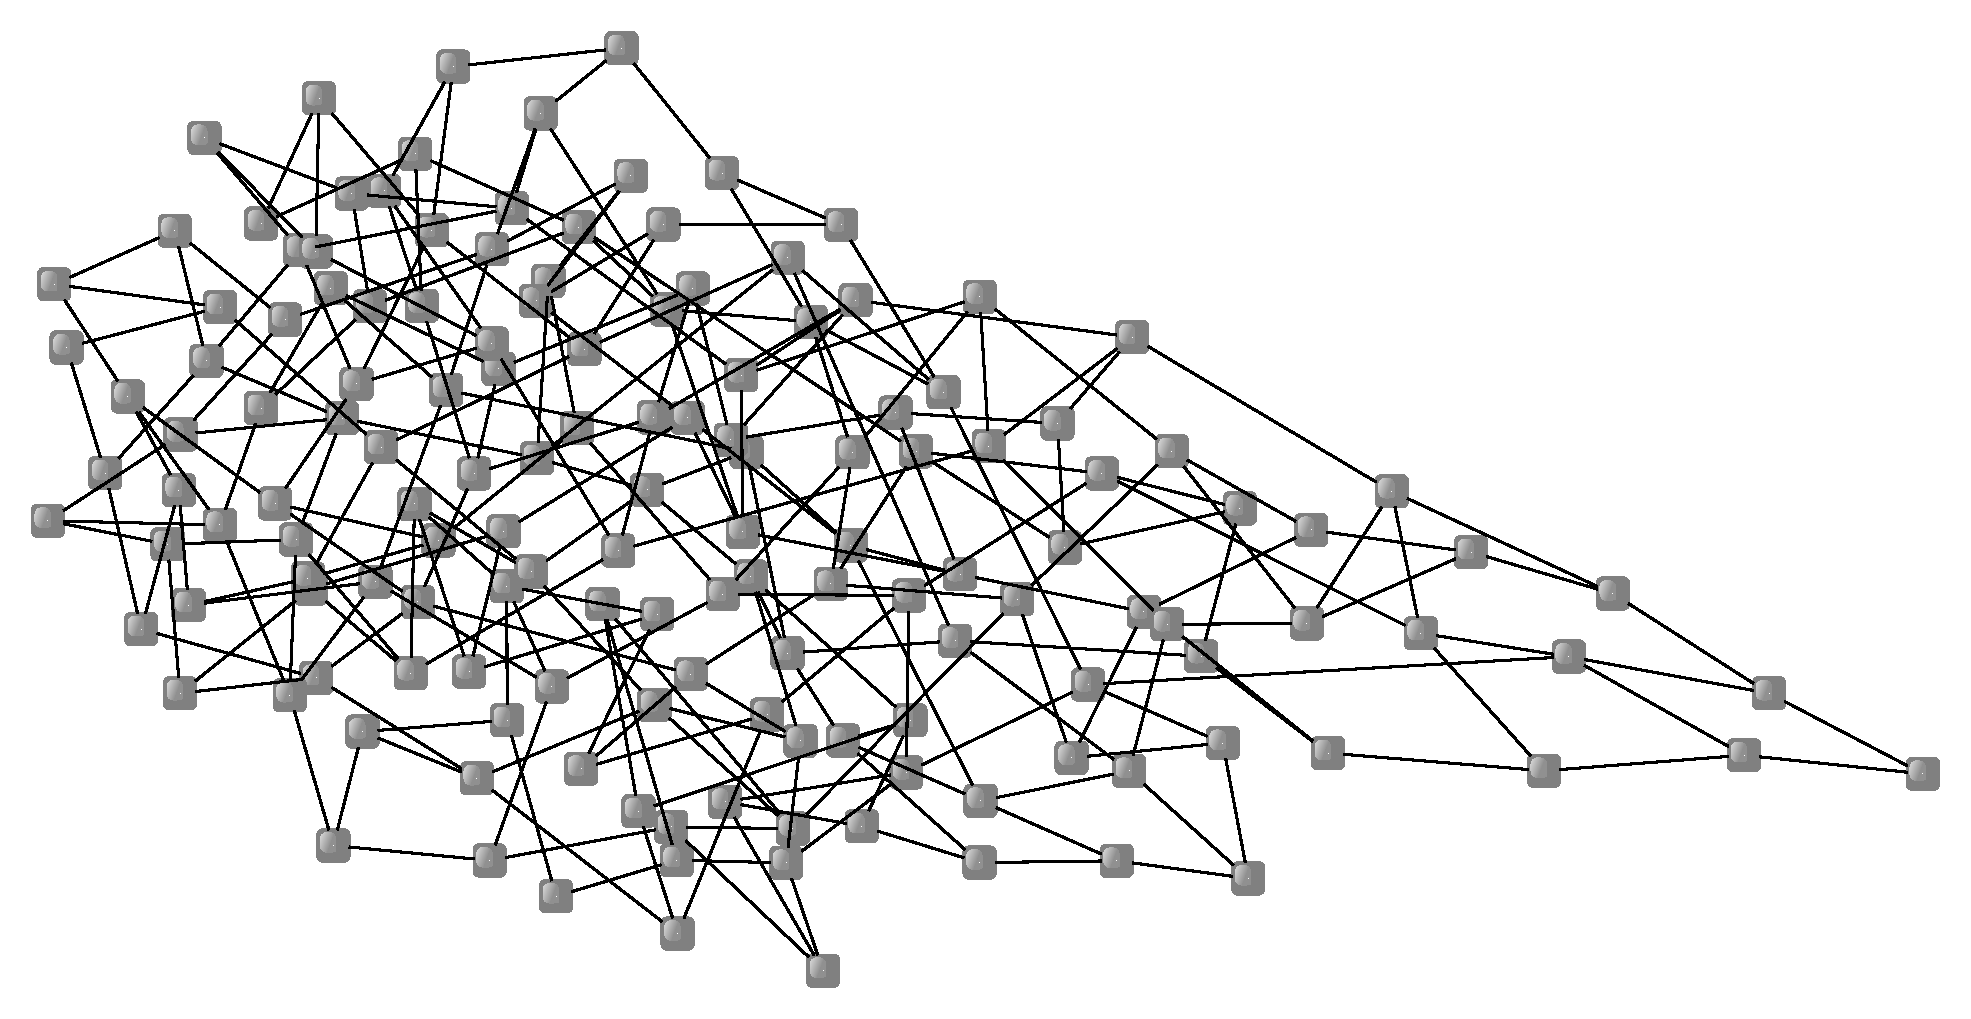
\includegraphics[width=0.27\textwidth]{graph9-argyriou-crossing}}
	\hfill
	\subfloat[\label{fig:graph9-argyriou-ar}{Angular Resolution}]{
	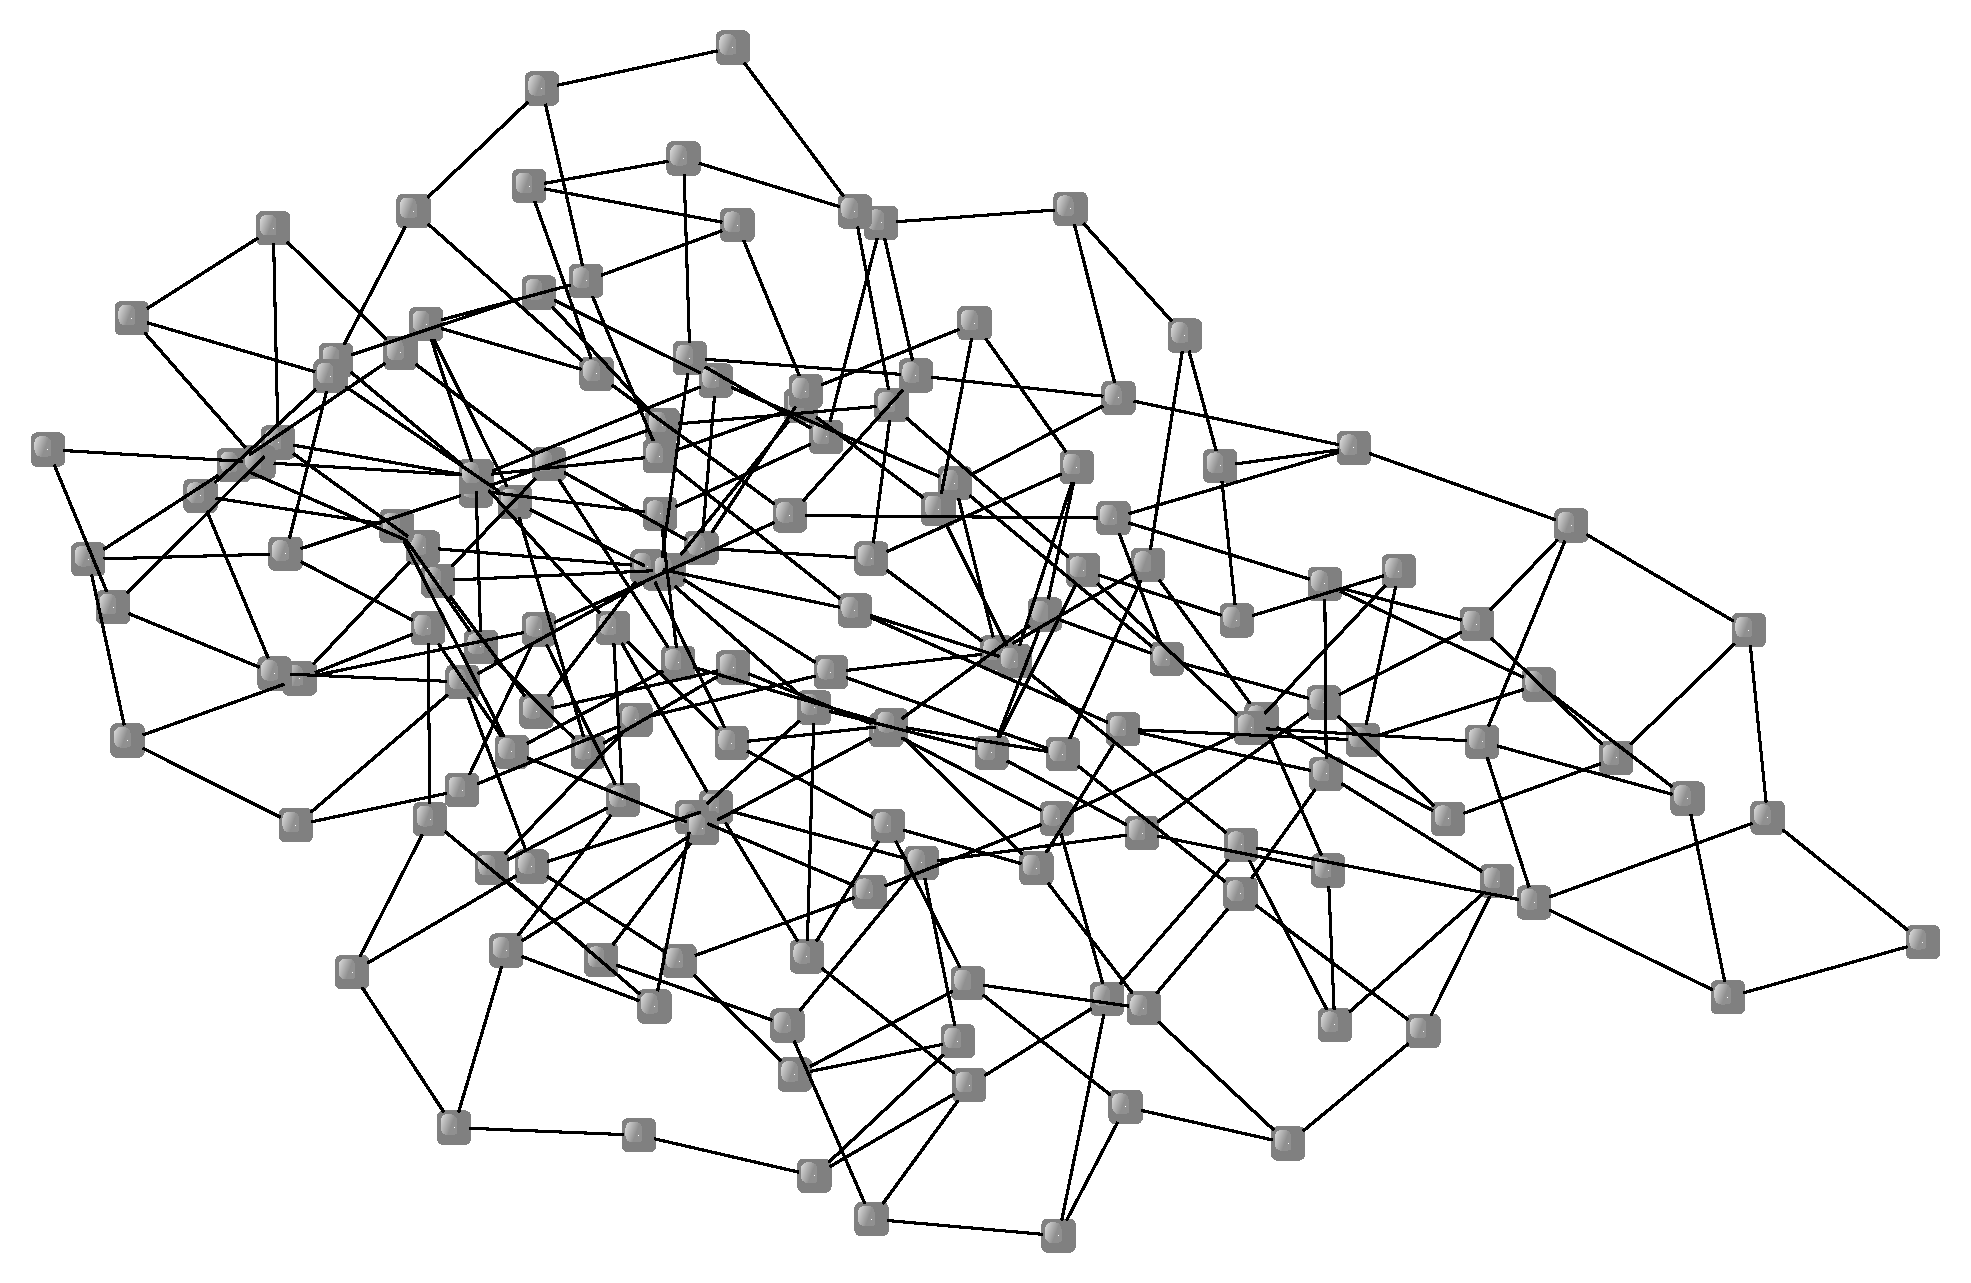
\includegraphics[width=0.27\textwidth]{graph9-argyriou-angular}}
	\hfill
	\subfloat[\label{fig:graph9-argyriou-tr}{Total Resolution}]{
	\includegraphics[width=0.27\textwidth]{graph9-argyriou-total}}	
	\hfill
	\subfloat[\label{fig:graph9-huang-cr}{Crossing Resolution}]{
	\includegraphics[width=0.27\textwidth]{graph9-huang-crossing}}
	\hfill
	\subfloat[\label{fig:graph9-huang-ar}{Angular Resolution}]{
	\includegraphics[width=0.27\textwidth]{graph9-huang-angular}}
	\hfill
	\subfloat[\label{fig:graph9-huang-tr}{Total Resolution}]{
	\includegraphics[width=0.27\textwidth]{graph9-huang-total}}
	\caption{Different drawings of the 9th challenge graph given in the Graph Drawing 2017 contest produced by different variants of
	(a)--(c)~the variant of our algorithm without restrictions on the aspect ratio, 
	(d)--(f)~the variant of our algorithm forced to maintain the input aspect ratio,
	(g)--(i)~the algorithm by Argyriou et al.~\cite{DBLP:journals/cj/ArgyriouBS13}, and
	(j)--(l)~the algorithm by Huang et al.~\cite{DBLP:journals/vlc/HuangEHL13}.
	Each variant was obtained by optimizing a different aesthetic criterion, which is named in the caption of each subfigure.}
	\label{fig:graph9}
\end{figure*}

\end{document}
